%% This is the ctufit-thesis example file. It is used to produce theses
%% for submission to Czech Technical University, Faculty of Information Technology.
%%
%% Get the newest version from
%% https://gitlab.fit.cvut.cz/theses-templates/FITthesis-LaTeX
%%
%%
%% Copyright 2021, Eliska Sestakova and Ondrej Guth
%%
%% This work may be distributed and/or modified under the
%% conditions of the LaTeX Project Public Licenese, either version 1.3
%% of this license or (at your option) any later version.
%% The latest version of this license is in
%%  https://www.latex-project.org/lppl.txt
%% and version 1.3 or later is part of all distributions of LaTeX
%% version 2005/12/01 or later.
%%
%% This work has the LPPL maintenance status `maintained'.
%%
%% The current maintainer of this work is Ondrej Guth.
%% Contact ondrej.guth@fit.cvut.cz for bug reports.
%% Alternatively, submit bug reports into the tracker at
%% https://gitlab.fit.cvut.cz/theses-templates/FITthesis-LaTeX/issues
%%
%%

%%%%%%%%%%%%%%%%%%%%%%%%%%%%%%%%%%%%%%%%%
% CLASS OPTIONS
% language: czech/english/slovak
% thesis type: bachelor/master/dissertation
%%%%%%%%%%%%%%%%%%%%%%%%%%%%%%%%%%%%%%%%%
\documentclass[english,master,unicode]{ctufit-thesis}

%%%%%%%%%%%%%%%%%%%%%%%%%%%%%%%%%%
% FILL IN THIS INFORMATION
%%%%%%%%%%%%%%%%%%%%%%%%%%%%%%%%%%
\ctufittitle{Meme Generator} % replace with the title of your thesis
\ctufitauthorfull{Bc. Ondřej Závodný} % replace with your full name (first name(s) and then family name(s) / surname(s)) including academic degrees
\ctufitauthorsurnames{Závodný} % replace with your surname(s) / family name(s)
\ctufitauthorgivennames{Ondřej} % replace with your first name(s) / given name(s)
\ctufitsupervisor{Ing. Michal Valenta, Ph.D.} % replace with name of your supervisor/advisor (include academic degrees)
\ctufitdepartment{Department of Software Engineering} % replace with the department of your defence
\ctufityear{2024} % replace with the year of your defence
\ctufitdeclarationplace{Prague} % replace with the place where you sign the declaration
\ctufitdeclarationdate{January 11, 2024} % replace with the date of signature of the declaration
\ctufitabstractCZE{Tato magisterská práce se zabývá vývojem aplikace pro správu šablon memů a nasledným generováním memů z těchto šablon. Jsou evaluovány existující generátory memů a popsána jejich funkcionalita. Výsledná aplikace je sestavena do docker image a poté nasazena do produkce. Aplikace byla otestována end-to-end testy a byla součástí usability testingu.}
\ctufitabstractENG{This masters thesis is focused on developing an application that enables management of meme templates and creating memes from them. It evaluates some existing meme generators and describes their functionality. The final application is built into a docker image and deployed to production. The application was tested using end-to-end tests and in usability testing.}
\ctufitkeywordsCZE{meme, memová šablona, editace obrázků, webová aplikace, frontend, nextjs, docker}
\ctufitkeywordsENG{meme, meme template, image editing, web application, frontend, nextjs, docker}
%%%%%%%%%%%%%%%%%%%%%%%%%%%%%%%%%%
% END FILL IN
%%%%%%%%%%%%%%%%%%%%%%%%%%%%%%%%%%

%%%%%%%%%%%%%%%%%%%%%%%%%%%%%%%%%%
% CUSTOMIZATION of this template
% Skip this part or alter it if you know what you are doing.
%%%%%%%%%%%%%%%%%%%%%%%%%%%%%%%%%%

\RequirePackage{iftex}[2020/03/06]
\iftutex % XeLaTeX and LuaLaTeX
    \RequirePackage{ellipsis}[2020/05/22] %ellipsis workaround for XeLaTeX
\else
    \RequirePackage[utf8]{inputenc}[2018/08/11] %this file encoding
    \RequirePackage{lmodern}[2009/10/30] % vector flavor of Computer Modern font
\fi

% hyperlinks
\RequirePackage[pdfpagelayout=TwoPageRight,colorlinks=false,allcolors=decoration,pdfborder={0 0 0.1}]{hyperref}[2020-05-15]

% uncomment the following to hide all hyperlinks
% \RequirePackage[pdfpagelayout=TwoPageRight,hidelinks]{hyperref}[2020-05-15]

\RequirePackage{pdfpages}[2020/01/28]

\setcounter{secnumdepth}{4} % numbering sections; 4: subsubsection



%%%%%%%%%%%%%%%%%%%%%%%%%%%%%%%%%%
% CUSTOMIZATION of this template END
%%%%%%%%%%%%%%%%%%%%%%%%%%%%%%%%%%


%%%%%%%%%%%%%%%%%%%%%%
% DEMO CONTENTS SETTINGS
% You may choose to modify this part.
%%%%%%%%%%%%%%%%%%%%%%
\usepackage{dirtree}
\usepackage{lipsum,tikz}
\usepackage{csquotes}
\usepackage[style=iso-numeric]{biblatex}
\addbibresource{text/bib-database.bib}
\usepackage{listings} % typesetting of sources
% \usepackage{minted} % typesetting of sources
\usepackage{tikz}
\usetikzlibrary{shapes.geometric, arrows}
\usepackage{subcaption}
\usepackage{dirtytalk}
\usepackage[acronym]{glossaries}
\usepackage{longtable}
\usepackage{array}
\usepackage{enumitem}
\usepackage{xcolor}
\usepackage{verbatim}

%theorems, definitions, etc.
\theoremstyle{plain}
\newtheorem{theorem}{Věta}
\newtheorem{lemma}[theorem]{Tvrzení}
\newtheorem{corollary}[theorem]{Důsledek}
\newtheorem{proposition}[theorem]{Návrh}
\newtheorem{definition}[theorem]{Definice}
\theoremstyle{definition}
\newtheorem{example}[theorem]{Příklad}
\theoremstyle{remark}
\newtheorem{note}[theorem]{Poznámka}
\newtheorem*{note*}{Poznámka}
\newtheorem{remark}[theorem]{Pozorování}
\newtheorem*{remark*}{Pozorování}
\numberwithin{theorem}{chapter}
%theorems, definitions, etc. END
%%%%%%%%%%%%%%%%%%%%%%
% DEMO CONTENTS SETTINGS END
%%%%%%%%%%%%%%%%%%%%%%

\newcommand{\myparagraph}[1]{\paragraph{#1}\mbox{}\\}
\newcommand{\tabitem}{~~\llap{\textbullet}~~}

\begin{document} 
\frontmatter\frontmatterinit % do not remove these two commands

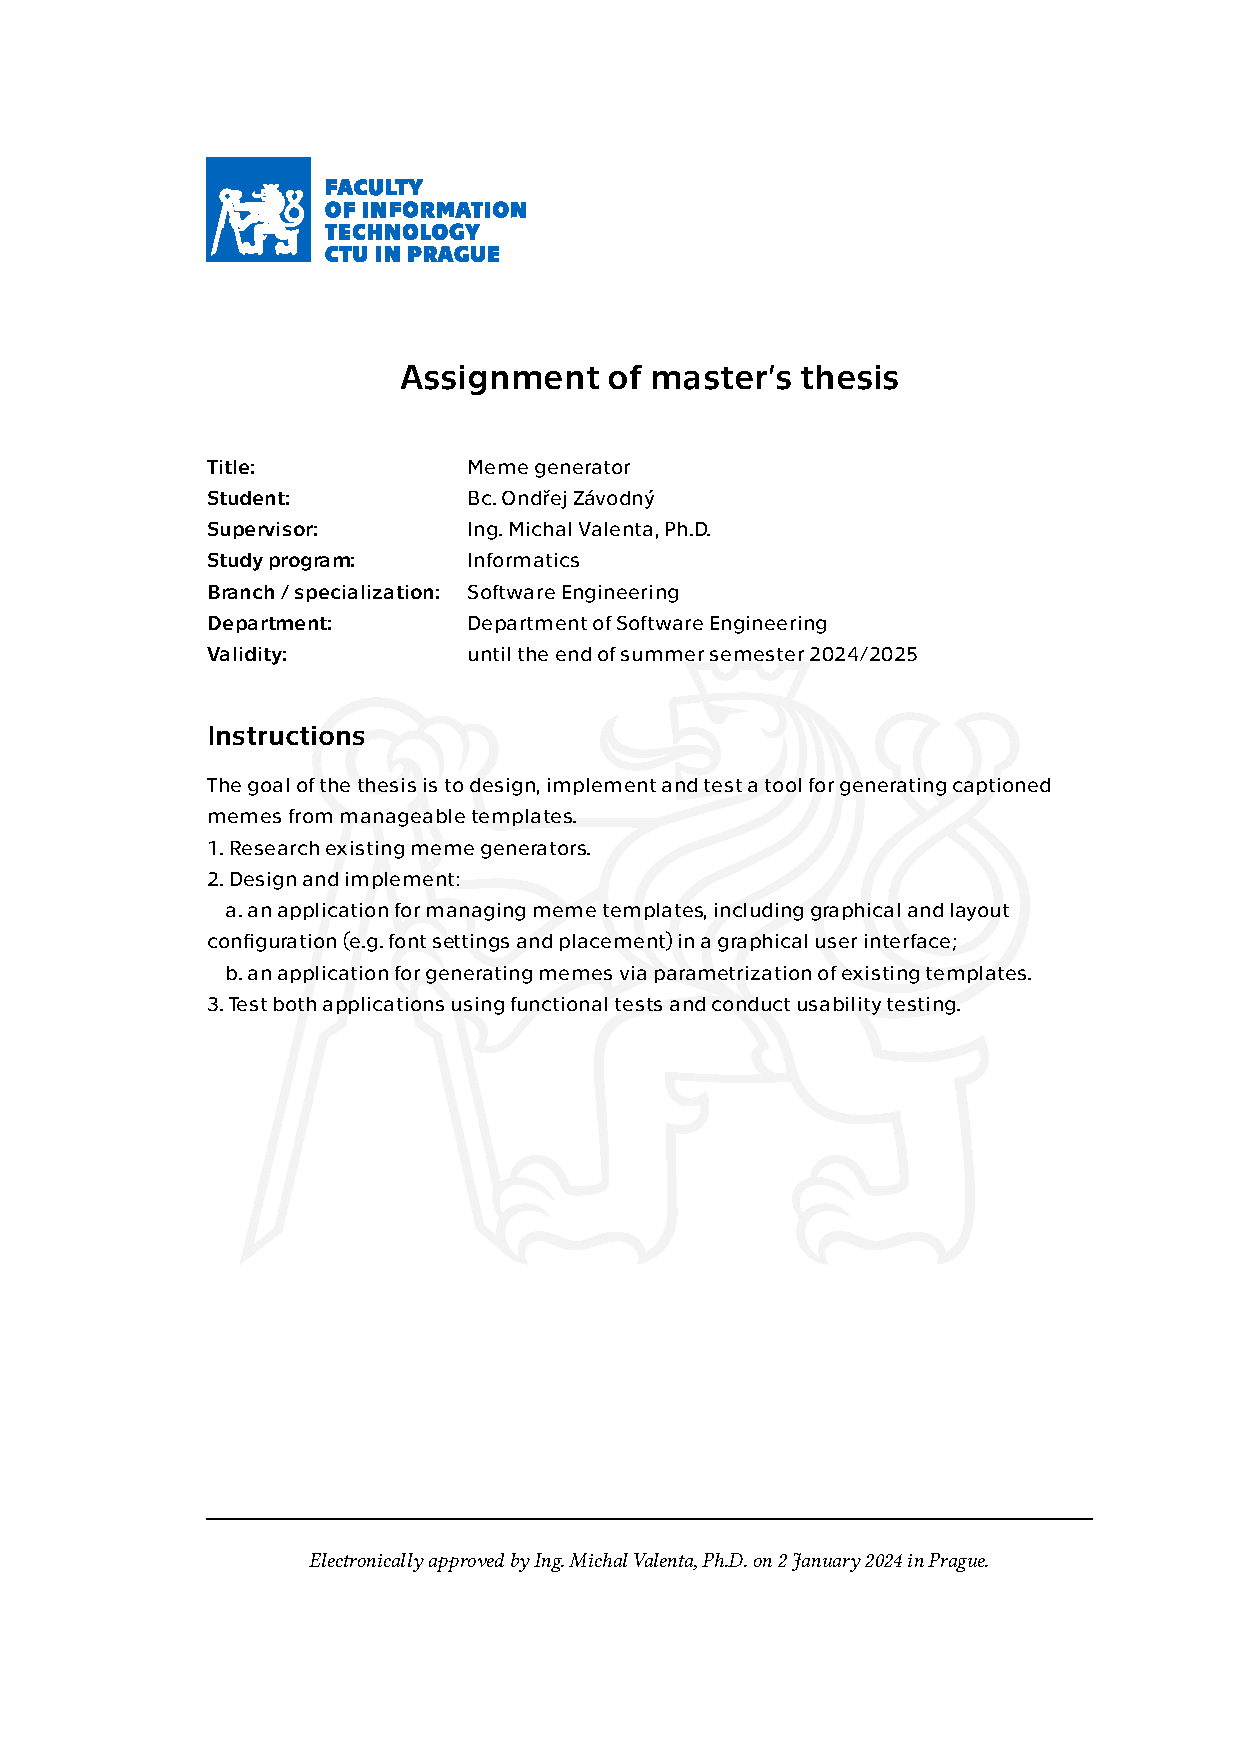
\includepdf{assignment-include.pdf} % replace that file with your thesis assignment provided by study office

\thispagestyle{empty}\cleardoublepage\maketitle % do not remove these three commands

\imprintpage % do not remove this command

\tableofcontents % do not remove this command
%%%%%%%%%%%%%%%%%%%%%%
% list of other contents: figures, tables, code listings, algorithms, etc.
% add/remove commands accordingly
%%%%%%%%%%%%%%%%%%%%%%
\listoffigures % list of figures
\begingroup
\let\clearpage\relax
\lstlistoflistings % list of source code listings generated by the listings package
% \listoflistings % list of source code listings generated by the minted package
\endgroup
%%%%%%%%%%%%%%%%%%%%%%
% list of other contents END
%%%%%%%%%%%%%%%%%%%%%%

%%%%%%%%%%%%%%%%%%%
% ACKNOWLEDGMENT
% FILL IN / MODIFY
% This is a place to thank people for helping you. It is common to thank your supervisor.
%%%%%%%%%%%%%%%%%%%
\begin{acknowledgmentpage}
	I would like to thank my fiancé for her support and also to Ing. Michal Valenta, Ph.D. for taking the time to help me with the thesis.
\end{acknowledgmentpage} 
%%%%%%%%%%%%%%%%%%%
% ACKNOWLEDGMENT END
%%%%%%%%%%%%%%%%%%%


%%%%%%%%%%%%%%%%%%%
% DECLARATION
% FILL IN / MODIFY
%%%%%%%%%%%%%%%%%%%
% INSTRUCTIONS
% ENG: choose one of approved texts of the declaration. DO NOT CREATE YOUR OWN. Find the approved texts at https://courses.fit.cvut.cz/SFE/download/index.html#_documents (document Declaration for FT in English)
% CZE/SLO: Vyberte jedno z fakultou schvalenych prohlaseni. NEVKLADEJTE VLASTNI TEXT. Schvalena prohlaseni najdete zde: https://courses.fit.cvut.cz/SZZ/dokumenty/index.html#_dokumenty (prohlášení do ZP)
\begin{declarationpage}
I hereby declare that the presented thesis is my own work and that I have cited all
sources of information in accordance with the Guideline for adhering to ethical
principles when elaborating an academic final thesis.
I acknowledge that my thesis is subject to the rights and obligations stipulated by the
Act No. 121/2000 Coll., the Copyright Act, as amended, in particular that the Czech
Technical University in Prague has the right to conclude a license agreement on the
utilization of this thesis as a school work under the provisions of Article 60 (1) of the
Act.
\end{declarationpage}
%%%%%%%%%%%%%%%%%%%
% DECLARATION END
%%%%%%%%%%%%%%%%%%%

\printabstractpage % do not remove this command

%%%%%%%%%%%%%%%%%%%
% SUMMARY
% FILL IN / MODIFY
% OR REMOVE ENTIRELY (upon agreement with your supervisor)
% (appropriate to remove in most theses)
%%%%%%%%%%%%%%%%%%%
% \begin{summarypage}
% \section*{Summary section}

% \lipsum[1][1-8]

% \end{summarypage}
%%%%%%%%%%%%%%%%%%%
% SUMMARY END
%%%%%%%%%%%%%%%%%%%

%%%%%%%%%%%%%%%%%%%
% ABBREVIATIONS
% FILL IN / MODIFY
% OR REMOVE ENTIRELY
% List the abbreviations in lexicography order.
%%%%%%%%%%%%%%%%%%%
% \chapter{Seznam zkratek}
	
% \begin{tabular}{rl}
% DFA & Deterministic Finite Automaton\\
% FA & Finite Automaton\\
% LPS & Labelled Prüfer Sequence\\
% NFA & Nondeterministic Finite Automaton\\
% NPS & Numbered Prüfer Sequence\\
% XML & Extensible Markup Language\\
% XPath & XML Path Language\\
% XSLT & eXtensible Stylesheet Language Transformations\\
% W3C & World Wide Web Consortium
% \end{tabular}
%%%%%%%%%%%%%%%%%%%
% ABBREVIATIONS END
%%%%%%%%%%%%%%%%%%%

\mainmatter\mainmatterinit % do not remove these two commands

%%%%%%%%%%%%%%%%%%%
% THE THESIS
% MODIFY ANYTHING BELOW THIS LINE
%%%%%%%%%%%%%%%%%%%

% Do not forget to include Introduction
%---------------------------------------------------------------
% \chapter{Introduction}
% uncomment the following line to create an unnumbered chapter
\chapter*{Introduction}\addcontentsline{toc}{chapter}{Introduction}\markboth{Introduction}{Introduction}
%---------------------------------------------------------------
\setcounter{page}{1}

\newacronym{api}{API}{Application Programming Interface}
\newacronym{orm}{ORM}{Object-relational mapping}

% The following environment can be used as a mini-introduction for a chapter. Use that any way it pleases you (or comment it out). It can contain, for instance, a summary of the chapter. Or, there can be a quotation.
% \begin{chapterabstract}
% \end{chapterabstract}

This thesis presents an in-depth exploration of one of the digital age's latest phenomenon: memes. The term "meme," originally coined by Richard Dawkins in 1976,\cite{meme}, originally described as small units of culture that spread from person to person by copying or imitation, has evolved in the internet era to describe images with text meant for sharing and virality.

The initial chapter offers an overview of current meme generators and introduces the developed application, setting the stage for a comparative analysis. The subsequent chapter delves into the technical aspects of the application's implementation, including the evaluation of frontend libraries, and the use of Docker for building and deploying the application.

Central to this study is the development and analysis of a web application designed for creating and sharing memes. This application enables users to generate memes using both existing templates and user-created designs, focusing on the ease of sharing these creations.

Concluding the thesis, the final chapter is devoted to testing, emphasizing end-to-end, component and usability testing methodologies. This ensures the application's functionality and user-friendliness, thereby highlighting the effectiveness of the developed solution in the broader context of digital meme creation.

%---------------------------------------------------------------
\chapter{Analysis}
%---------------------------------------------------------------

%%%%%%%%%%%%%%%%%%%%%%%%%%%%%%%%%%%%%%%%%%%%%%%
\section{Existing solutions}
%%%%%%%%%%%%%%%%%%%%%%%%%%%%%%%%%%%%%%%%%%%%%%%

There are many solutions online that allow users to create memes from templates.\cite{imgflip-1} These solutions are usually free to use, but they offer some extra features that are locked behind a subscription. The subscription usually unlocks the ability to remove the watermark from the generated memes, or the ability to use the application without ads. Two websites were chosen for a more detailed analysis, Imgflip and iLoveIMG. Imgflip is consistently ranked as one of the most popular meme generators on the internet\cite{imgflip-1}\cite{imgflip-2}, and iLoveIMG is one of the easiest sites to use when an inexperienced user wants to create a meme.\cite{imgflip-1} In the mobile application space, Mematic was chosen for a more detailed analysis, because it is often mentioned as one of the best meme generators on the market.\cite{mematic-1}\cite{mematic-2}\cite{mematic-3}

\subsection{Popularity}

\begin{figure}
    \centering
    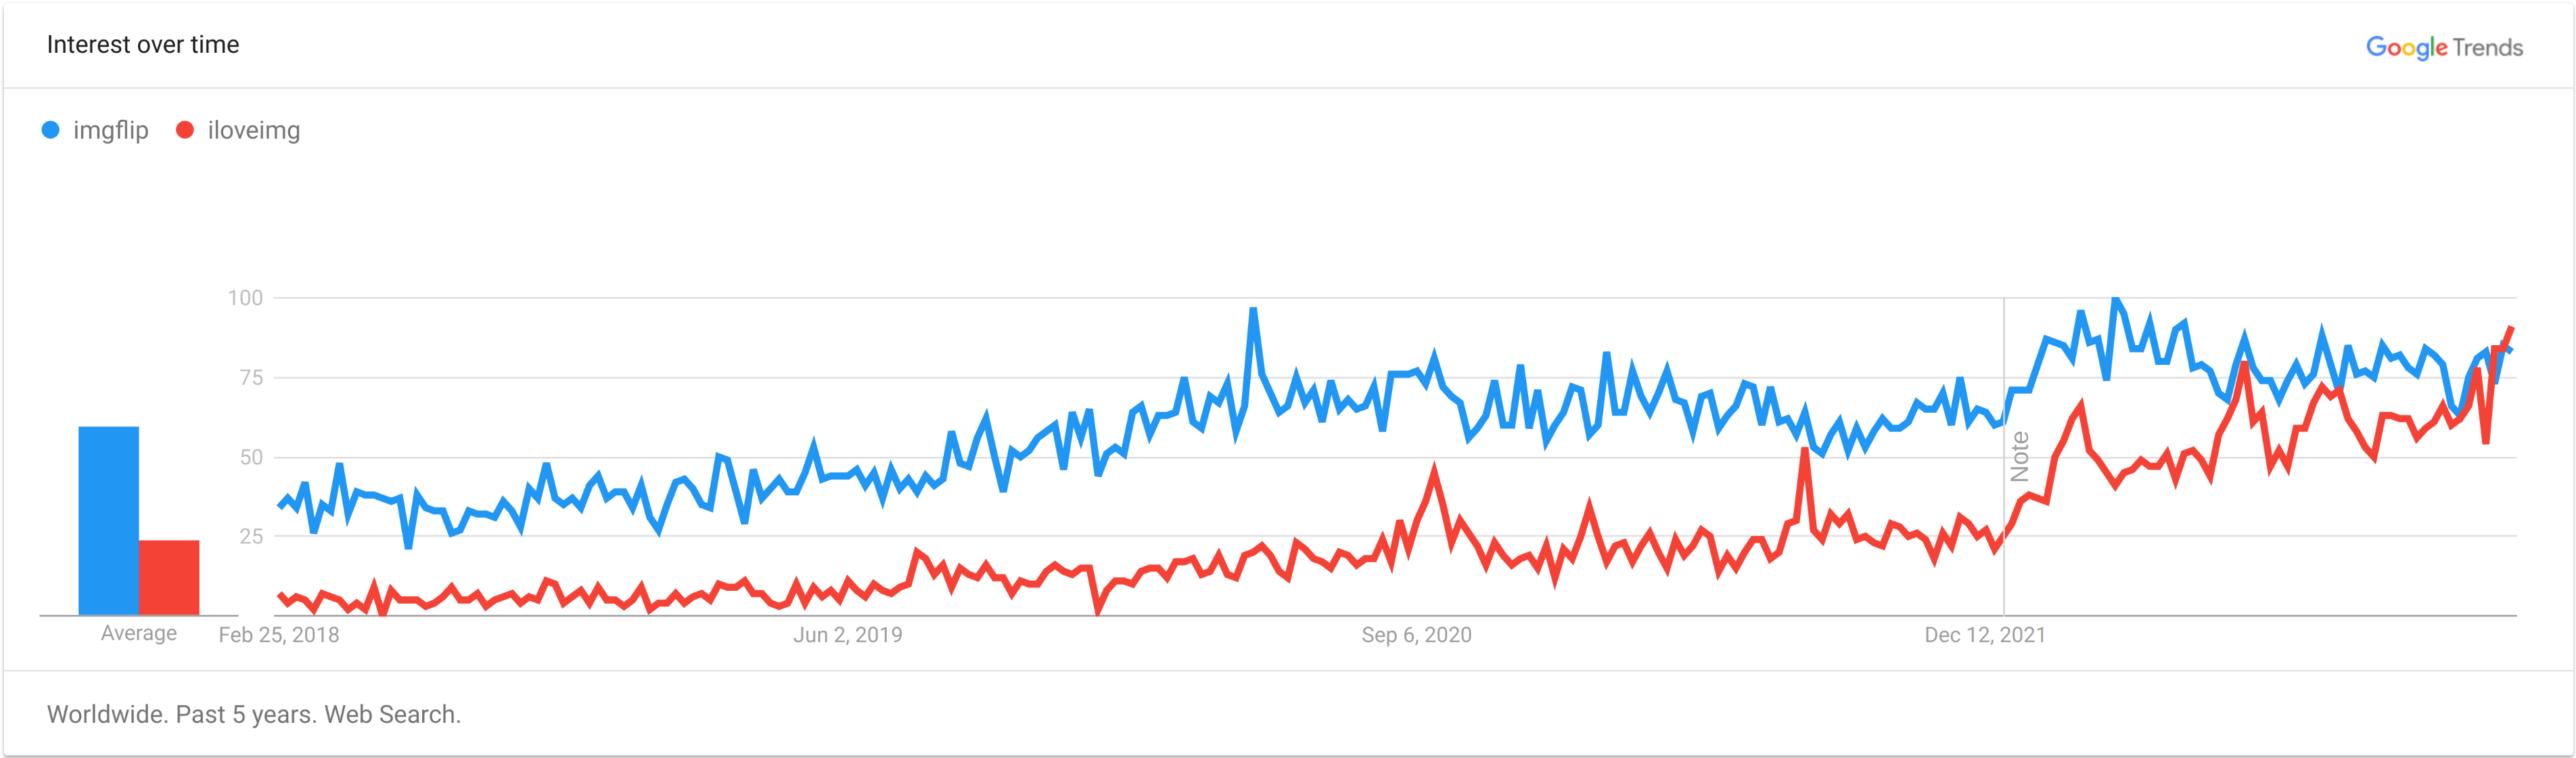
\includegraphics[width=\linewidth]{text/img/meme_trends.png}
    \caption{\label{fig:meme-trends}Google Trends for the search terms \texttt{imgflip} and \texttt{iloveimg} for the past 5 years. Taken on February 21. 2023.\cite{trends.google.com}}
\end{figure}

Popularity is difficult to find for websites. Android and iOS applications have a ranking system and a rough number of downloads listed in the respective stores, which can be used together to gain an insight into the popularity. Websites do not have such options, but search engines, like google, track search terms and make them available for analysis. Google offers the Google Trends, which shows how many times was each search term was searched in Google. Since this is not at all comparable to the any of the Android/iOS application metrics, websites and applications will not be compared between each other in this section.

A graph from Google Trends is shown in the image \ref{fig:meme-trends}, which shows that Imgflip was more searched than iLoveIMG for the past 5 years, except for January and February 2023, so it can be said that Imgflip is more popular than iLoveIMG.

Mematic has over 1 Million downloads on 48.9 Thousand reviews on Google Play\cite{mematic-google} and 150.1 Thousand reviews on the App Store\cite{mematic-apple}.

\subsection{Imgflip Meme Generator}

\begin{figure}
    \centering
    \begin{subfigure}{\textwidth}
        \centering
        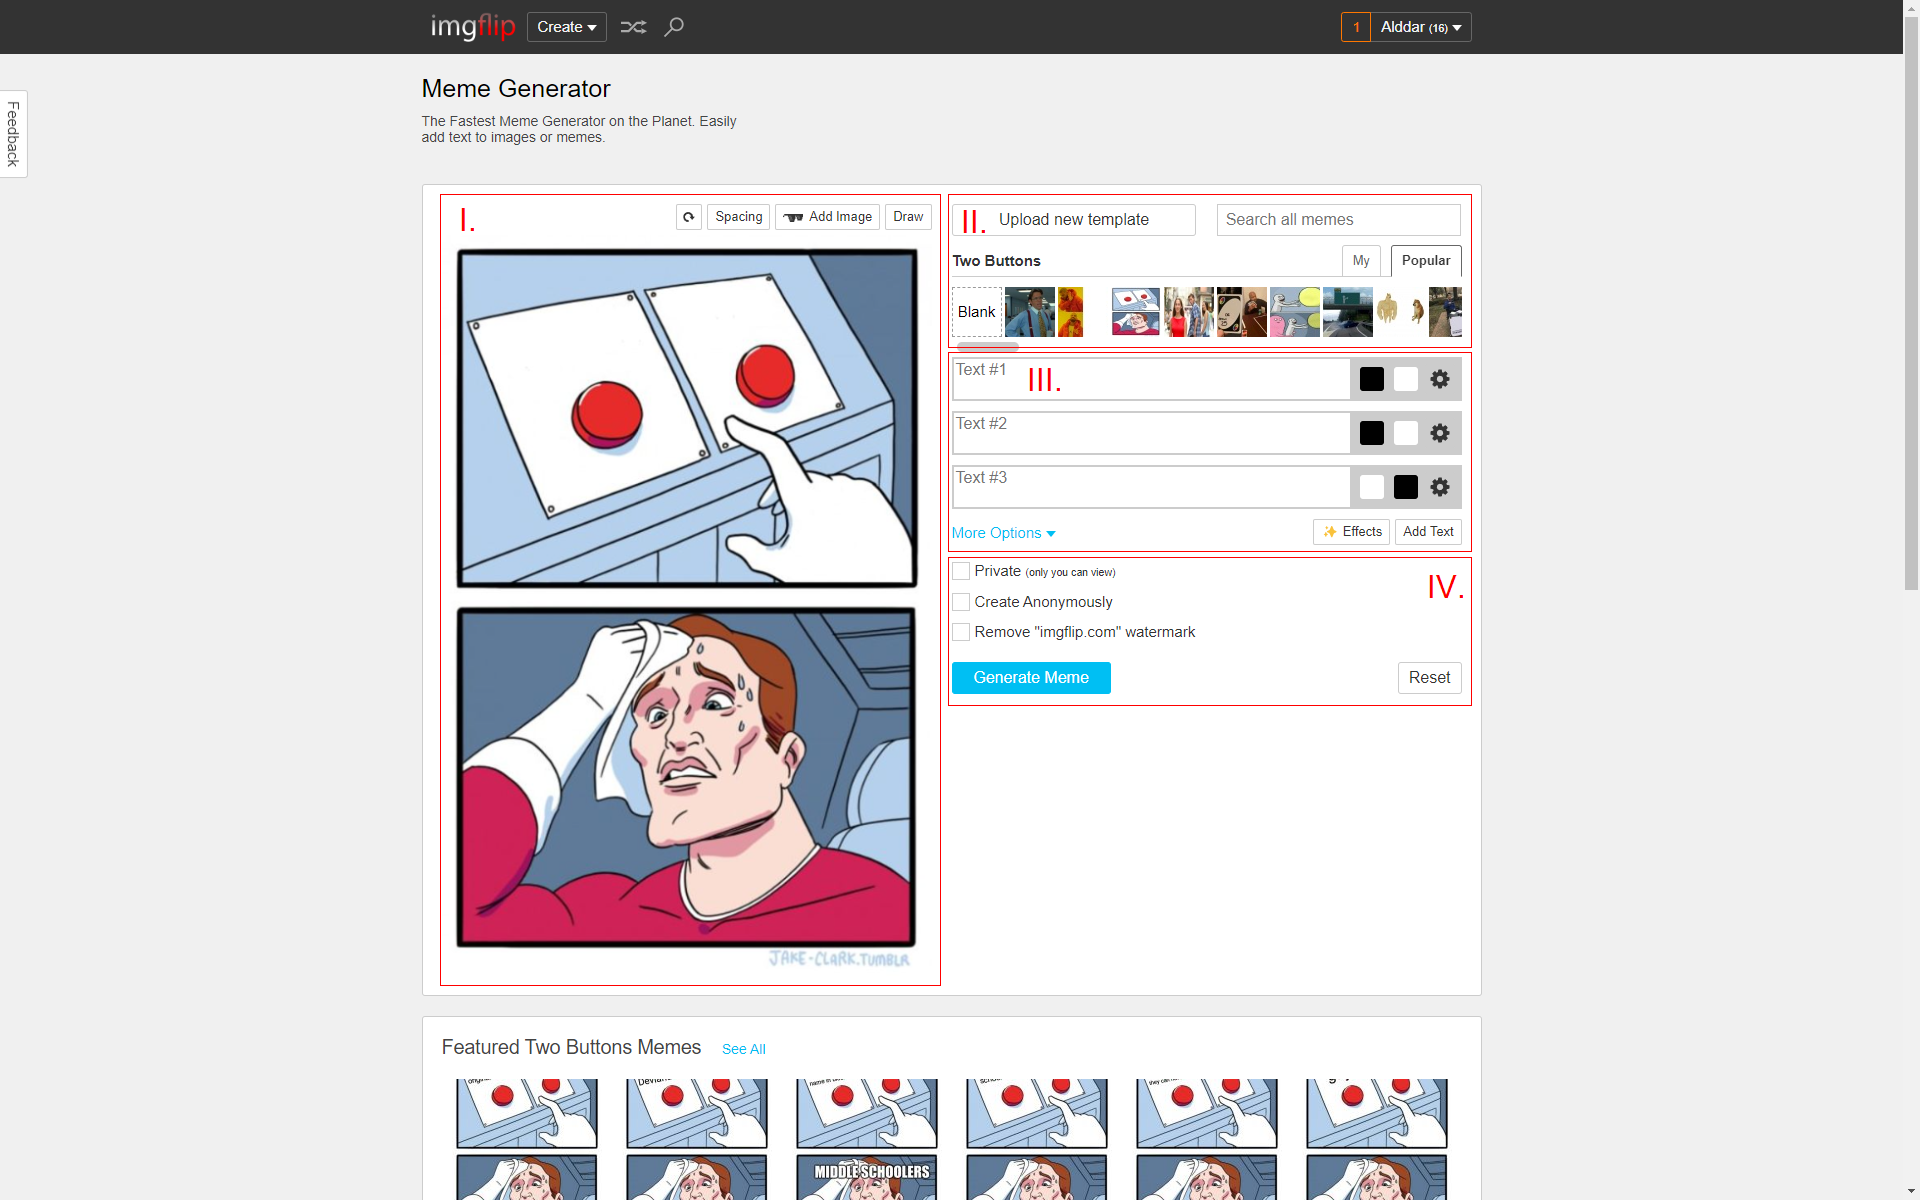
\includegraphics[width=\textwidth]{text/img/imgflip/main.png}
        \caption{Main Imgflip meme generator screen.}
        \label{fig:imgflip-main}
    \end{subfigure}
    % \end{figure}
    % \begin{figure}\ContinuedFloat
    \begin{subfigure}{0.3\textwidth}
        \centering
        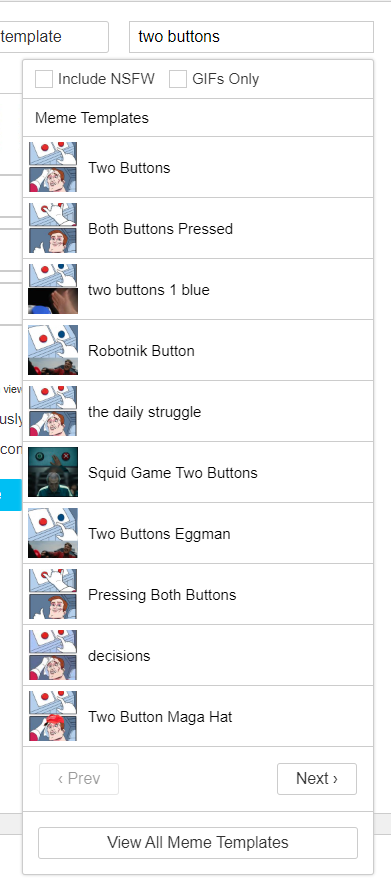
\includegraphics[width=\linewidth]{text/img/imgflip/search.png}
        \caption{Search dialog}
        \label{fig:imgflip-search}
    \end{subfigure}
    \begin{subfigure}{0.3\textwidth}
        \centering
        \raisebox{5mm}{
\includegraphics[width=\linewidth]{text/img/imgflip/generated-meme.png}}
        \caption{Generated meme dialog.}
        \label{fig:imgflip-generated-meme}
    \end{subfigure}
    \begin{subfigure}{0.3\textwidth}
        \centering
        \raisebox{18mm}{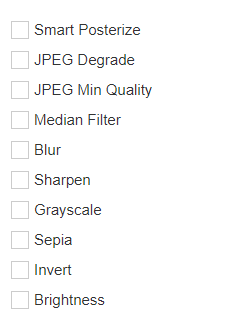
\includegraphics[width=\linewidth]{text/img/imgflip/effects.png}}
        \caption{Available effects}
        \label{fig:imgflip-effects}
    \end{subfigure}
\end{figure}
\begin{figure}\ContinuedFloat
    \begin{subfigure}{0.4\textwidth}
        \centering
        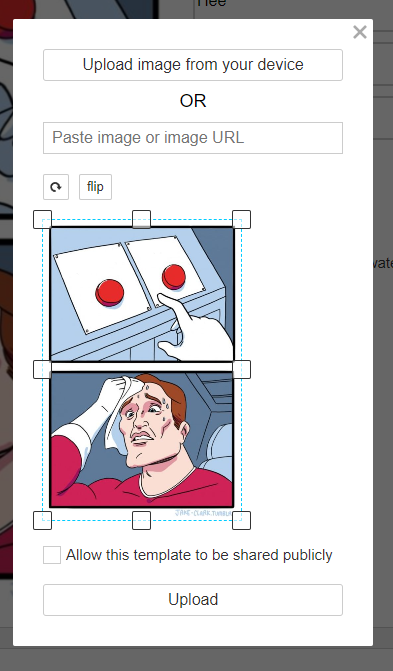
\includegraphics[width=\linewidth]{text/img/imgflip/upload-dialog.png}
        \caption{Upload dialog}
        \label{fig:imgflip-upload-dialog}
    \end{subfigure}
    \begin{subfigure}{0.4\textwidth}
        \centering
        \raisebox{10mm}{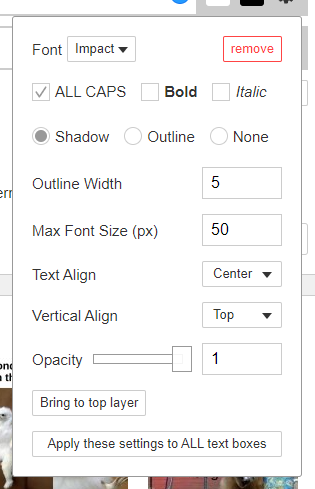
\includegraphics[width=\linewidth]{text/img/imgflip/text-properties.png}}
        \caption{Text Options}
        \label{fig:imgflip-text-options}
    \end{subfigure}
    \caption{Screenshots of Imgflip}
    \label{fig:imgflip}
\end{figure}

Imgflip Meme Generator \footnote{https://imgflip.com/memegenerator} is a free online image maker that lets users add custom resizable text, images, and much more to templates. The generator can be used to customize established memes, such as those found in Imgflip's collection of Meme Templates \footnote{https://imgflip.com/memetemplates}. It is also possible to upload custom templates or start from scratch with empty templates \cite{imgflip}.

\subsubsection{Creating a meme}

The main Imgflip screen is shown in the image \ref{fig:imgflip-main}. The image is split into four sections labeled with Roman numerals.

\myparagraph{Section I}

Section I. is the graphical editor of memes. There are 4 buttons at the top that can be used to manipulate the image. The first button rotates the whole image. The second button adds space, either to the top or to the button of the image. The third button allows the users to add some other images onto the background. The last button is used to draw on the image manually, being able to change the color and the thickness of the drawing tool. Below these buttons is the graphical editor. Here the user can move, rotate and resize text fields and images added to the meme.

\myparagraph{Section II}

Section II. is where the user can upload a new template (see \autoref{sec:imgflip-uploading-template}), or select from one of the many templates made by other users. There are two tabs with templates, one has all the templates created by the current user and the other one has a selection of the most popular templates on the platform. There is also a search bar. If the user starts typing, a search dialog, which is shown in image \ref{fig:imgflip-search}, will appear. It has pictures and names of all the relevant search results.

\myparagraph{Section III}

Section I. is where the user modifies other attributes of the image, mainly the texts. Each text field in section I. corresponds to a text box in the graphical image editor in section I. When any property in section III is changed, it is automatically updated in Section I. as well. The main text options are the actual text, its color and its outline color. The settings icon shows a dialog depicted in image \ref{fig:imgflip-text-options}, which contains many more text options, like font, outline width, max font size and others. There isn't an option for font size, the text will always try to take up the maximum available space, but it is possible to specify a maximum font size. Below the text options is the \texttt{Add text} button and the \texttt{Effects} button. There are many effects to choose from, as shown in image \ref{fig:imgflip-effects}.

\myparagraph{Section IV.}

Section IV. is the final publishing of the meme. There is an option to make the meme private and also the option to create the meme anonymously. There is also an option to not have the \texttt{imgflip.com} watermark on the final generated meme, but that isn't available without getting a subscription (see \autoref{sec:imgflip-subscriptions})


\subsubsection{Uploading a template}
\label{sec:imgflip-uploading-template}

\newacronym{url}{URL}{Uniform Resource Locator}

When the user clicks the \say{Upload new template} button, an upload dialog opens. This dialog is depicted in image \ref{fig:imgflip-upload-dialog}. Here there are three possible ways to upload an image. The first one is to select it from the device. The second one is to paste an \acrfull{url} to the desired image. The third one is to paste an image from the clipboard.

After an image is uploaded, it can be flipped, rotated and cropped. There is also an option to make this template public, which means it will be accessible to other users of the platform.


\subsubsection{Generating a meme}

When the \texttt{generate meme} button is clicked, it shows the generated meme dialog shown in image \ref{fig:imgflip-generated-meme}. The generated image is at the top of the dialog. There are many possible ways how to share the meme with people using several social networks and means of communication. The dialog has a generated link to the image and also an HTML code. There is also a \texttt{Submit this image to the Imgflip community} link, which would post it on the Imgflip social network.

\subsubsection{Subscriptions}
\label{sec:imgflip-subscriptions}

Imgflip is free to use, but it offers some extra features which are locked behind an \say{Imgflip Pro} subscription. The features that are available for the Meme Generator in the Pro version are the ability to remove the \say{imgflip.com} watermark from generated memes and the ad-free version of the page. There are also many other features for the other Imgflip products, like the Animated GIF Maker, which aren't a part of this thesis.

\subsection{Iloveimg Meme Generator}

\begin{figure}
    \centering
    \begin{subfigure}{\textwidth}
        \centering
        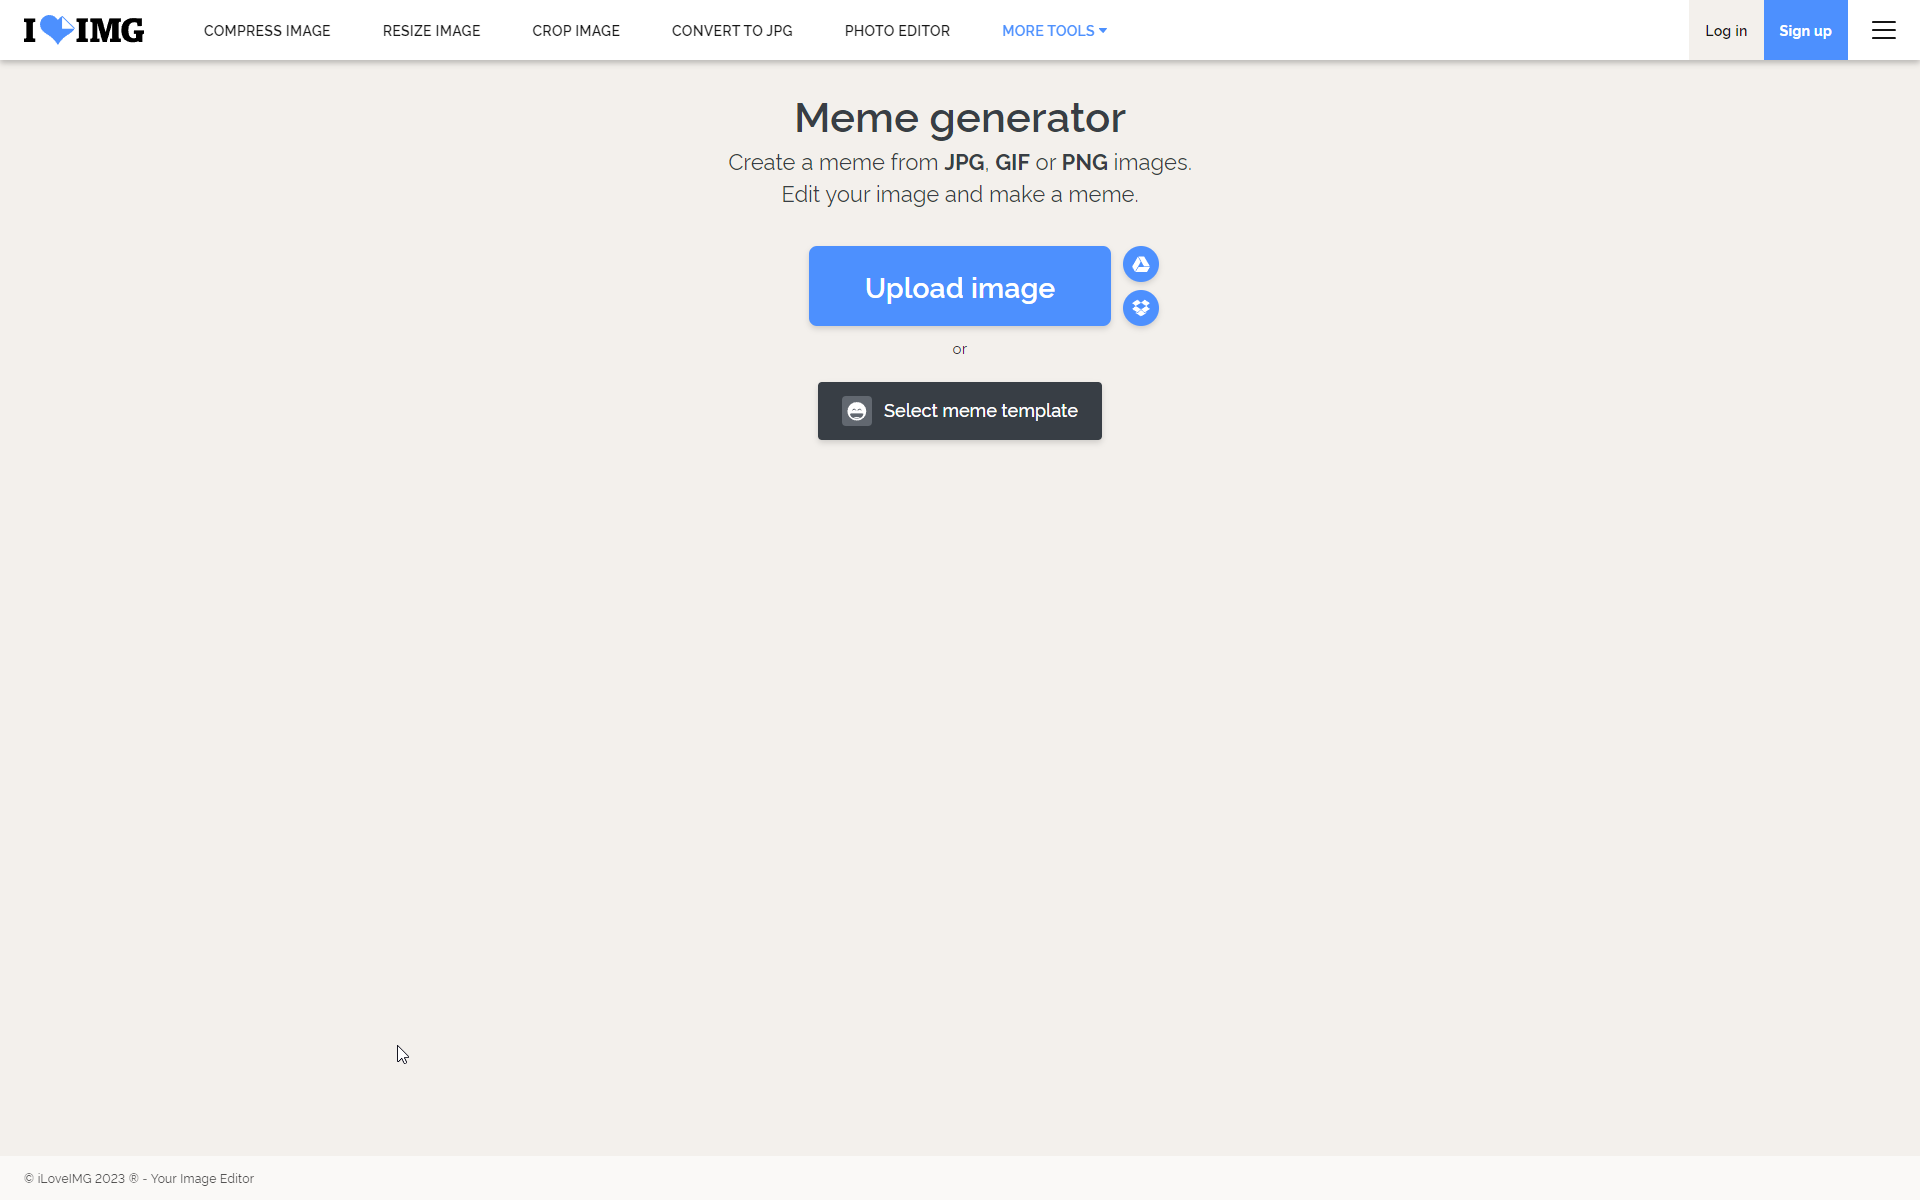
\includegraphics[width=\textwidth]{text/img/iloveimg/main.png}
        \caption{Main iLoveIMG meme generator screen.}
        \label{fig:iloveimg-main}
    \end{subfigure}
    \begin{subfigure}{\textwidth}
        \centering
        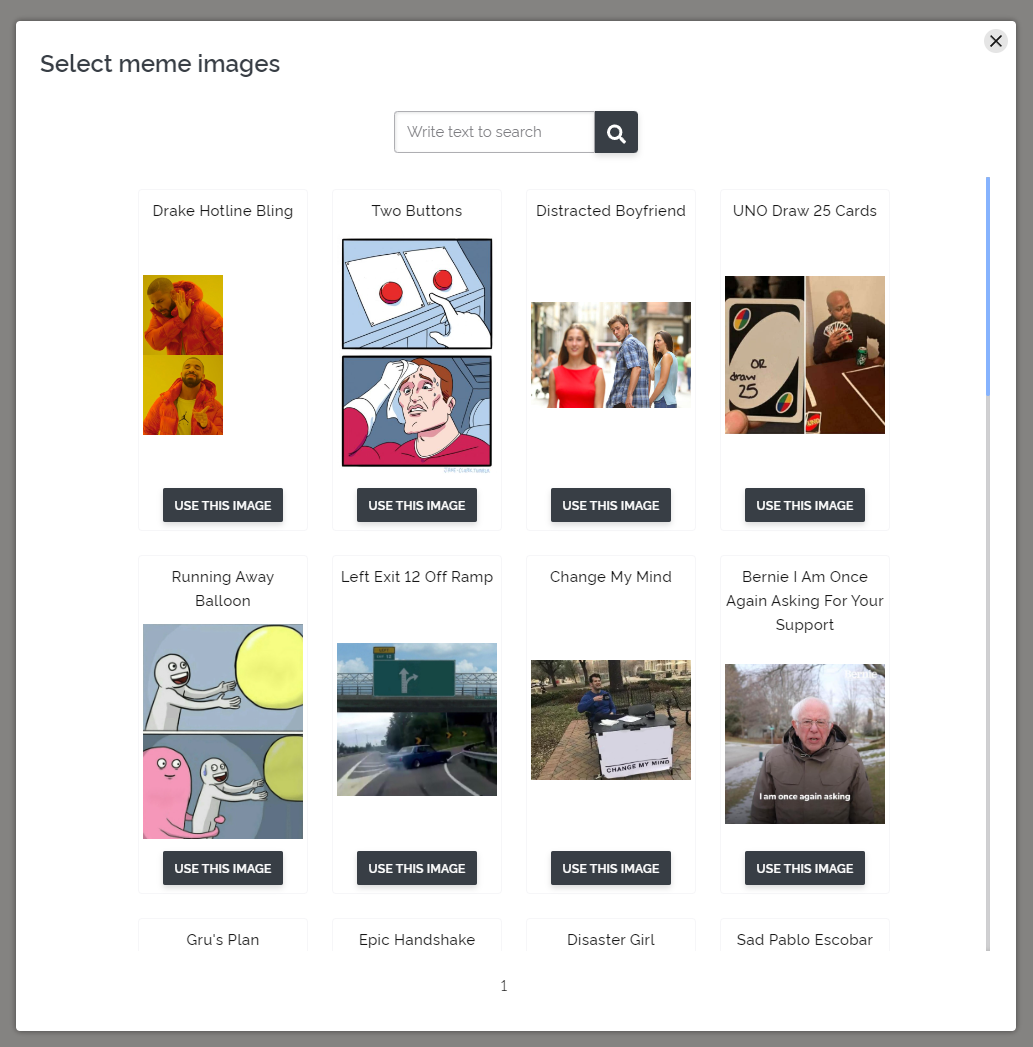
\includegraphics[width=\textwidth]{text/img/iloveimg/select-meme-dialog.png}
        \caption{Select meme dialog.}
        \label{fig:iloveimg-select-meme}
    \end{subfigure}
\end{figure}
\begin{figure}\ContinuedFloat
    \begin{subfigure}{\textwidth}
        \centering
        
\includegraphics[width=\textwidth]{text/img/iloveimg/editor.png}
        \caption{Meme editor.}
        \label{fig:iloveimg-meme-editor}
    \end{subfigure}
    \begin{subfigure}{\textwidth}
        \centering
        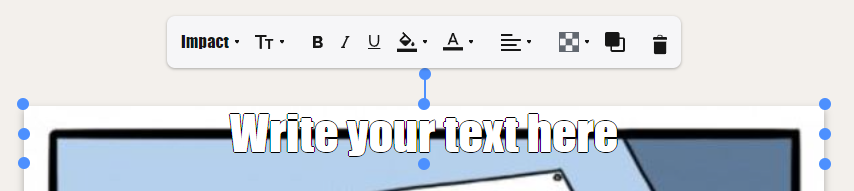
\includegraphics[width=\linewidth]{text/img/iloveimg/text-edit.png}
        \caption{Text editing tools}
        \label{fig:iloveimg-text-edit}
    \end{subfigure}
\end{figure}
\begin{figure}\ContinuedFloat
    \begin{subfigure}{\textwidth}
        \centering
        
\includegraphics[width=\textwidth]{text/img/iloveimg/generated-meme.png}
        \caption{Generated meme}
        \label{fig:iloveimg-generated-meme}
    \end{subfigure}
    \caption{Screenshots of iLoveIMG}
    \label{fig:iloveimg}
\end{figure}

ILoveIMG Meme Generator \footnote{https://www.iloveimg.com/meme-generator} is a part of the iLoveIMG suite of free tools designed to make working with images easy \cite{iloveimg-features}.

\subsubsection{Creating a meme}

The intro screen to the generator, shown in image \ref{fig:iloveimg-main}, asks the user to upload a custom image, or to select from predefined meme templates. When the user clocks the \texttt{Select meme template} button, the dialog shown in image \ref{fig:iloveimg-select-meme} appears. Here the user can select their desired template and use the search function to filter by name.

When the background is selected, the screen shown in image \ref{fig:iloveimg-meme-editor} appears. Here, the user can use the graphical editor to edit the meme. Every template comes with two default texts, one on the bottom and one on the top. The user can switch between the texts being positioned inside the image or outside the image by using the buttons on the right. Unlike Imgflip, the template does not come with texts placed in strategic places in the template, the user has to add and position the texts themselves.

Upon clicking on a text, a box with texts options appears on the top, shown on image \ref{fig:iloveimg-text-edit}. This allows the user to modify other properties of the text, such as the font, text size, colors, and others. There are also buttons to duplicate the text and to delete the text.

\subsubsection{Downloading a meme}

When the user clicks the \texttt{Generate MEME} button, they are redirected to the page shown in image \ref{fig:iloveimg-generated-meme}. There is an option to download the image, or save it directly to supported cloud storage solutions, like Dropbox. There are also social media buttons to share the image on social networks. There are also buttons to further work with the image using other tools which are part of the iLoveIMG portfolio, such as cropping, compressing or resizing the image \cite{iloveimg-features}.

\subsubsection{Subscriptions}

ILoveIMG offers a subscription to unlock more features throughout all their applications, like an ad-free version of the site or customer support. The benefit of having the paid subscription for the meme generator is the ability to create images with files of up to four gigabytes, where the free version only supports files up to two hundred megabytes \cite{iloveimg-pricing}

\subsection{Mematic}

Mematic is a free Android/iOS smartphone application for making memes, postcards, collages, and more. It offers controls adjusted for mobile phone usage.

\subsubsection{Creating a meme}

The initial screen of the application is shown in image \ref{fig:mematic-initial}. It shows many options on how to start editing images, where some options are hidden behind the pro subscription (see \autoref{sec:mematic-subscription}). The \texttt{Free Style} option is the most similar to the featured web applications.

When the \texttt{Free Style} option is selected, the template selection screen shows up as shown in image \ref{fig:mematic-template-selection}. Here, the user can scroll through many available templates, or use the search bar to filter the template selection.

After the user selects a template, the editing screen, shown in image \ref{fig:mematic-meme-edit}, shows up. The template comes with texts positioned according to the meme template. The bottom row of actions allows the users to add texts, add images and modify the watermark. The watermark modification is not a part of the free version, but it is unlocked with the pro subscription.

When the user double-taps a text, the text editing options show up, as depicted on image \ref{fig:mematic-text-edit}. The user can move, resize, rotate or remove the text in the graphical section. The bottom row of action also changes to offer other text editing options, like fonts, colors, or sizes.

\subsubsection{Exporting a meme}

When the user clicks the \texttt{Export} button, an export screen comes up, shown on image \ref{fig:mematic-export}. There is an option to remove the watermark, as well as to share or save the generated image. The \texttt{Share} button opens up the operating system sharing dialog.

\subsubsection{Subscriptions}
\label{sec:mematic-subscription}

Mematic offers a paid subscription to unlock additional features. The subscription includes access to all the fonts, the possibility to customize the watermark, an ad-free version of the application and others.

\begin{figure}
    \centering
    % \end{figure}
    % \begin{figure}\ContinuedFloat
    \begin{subfigure}{0.3\textwidth}
        \centering
        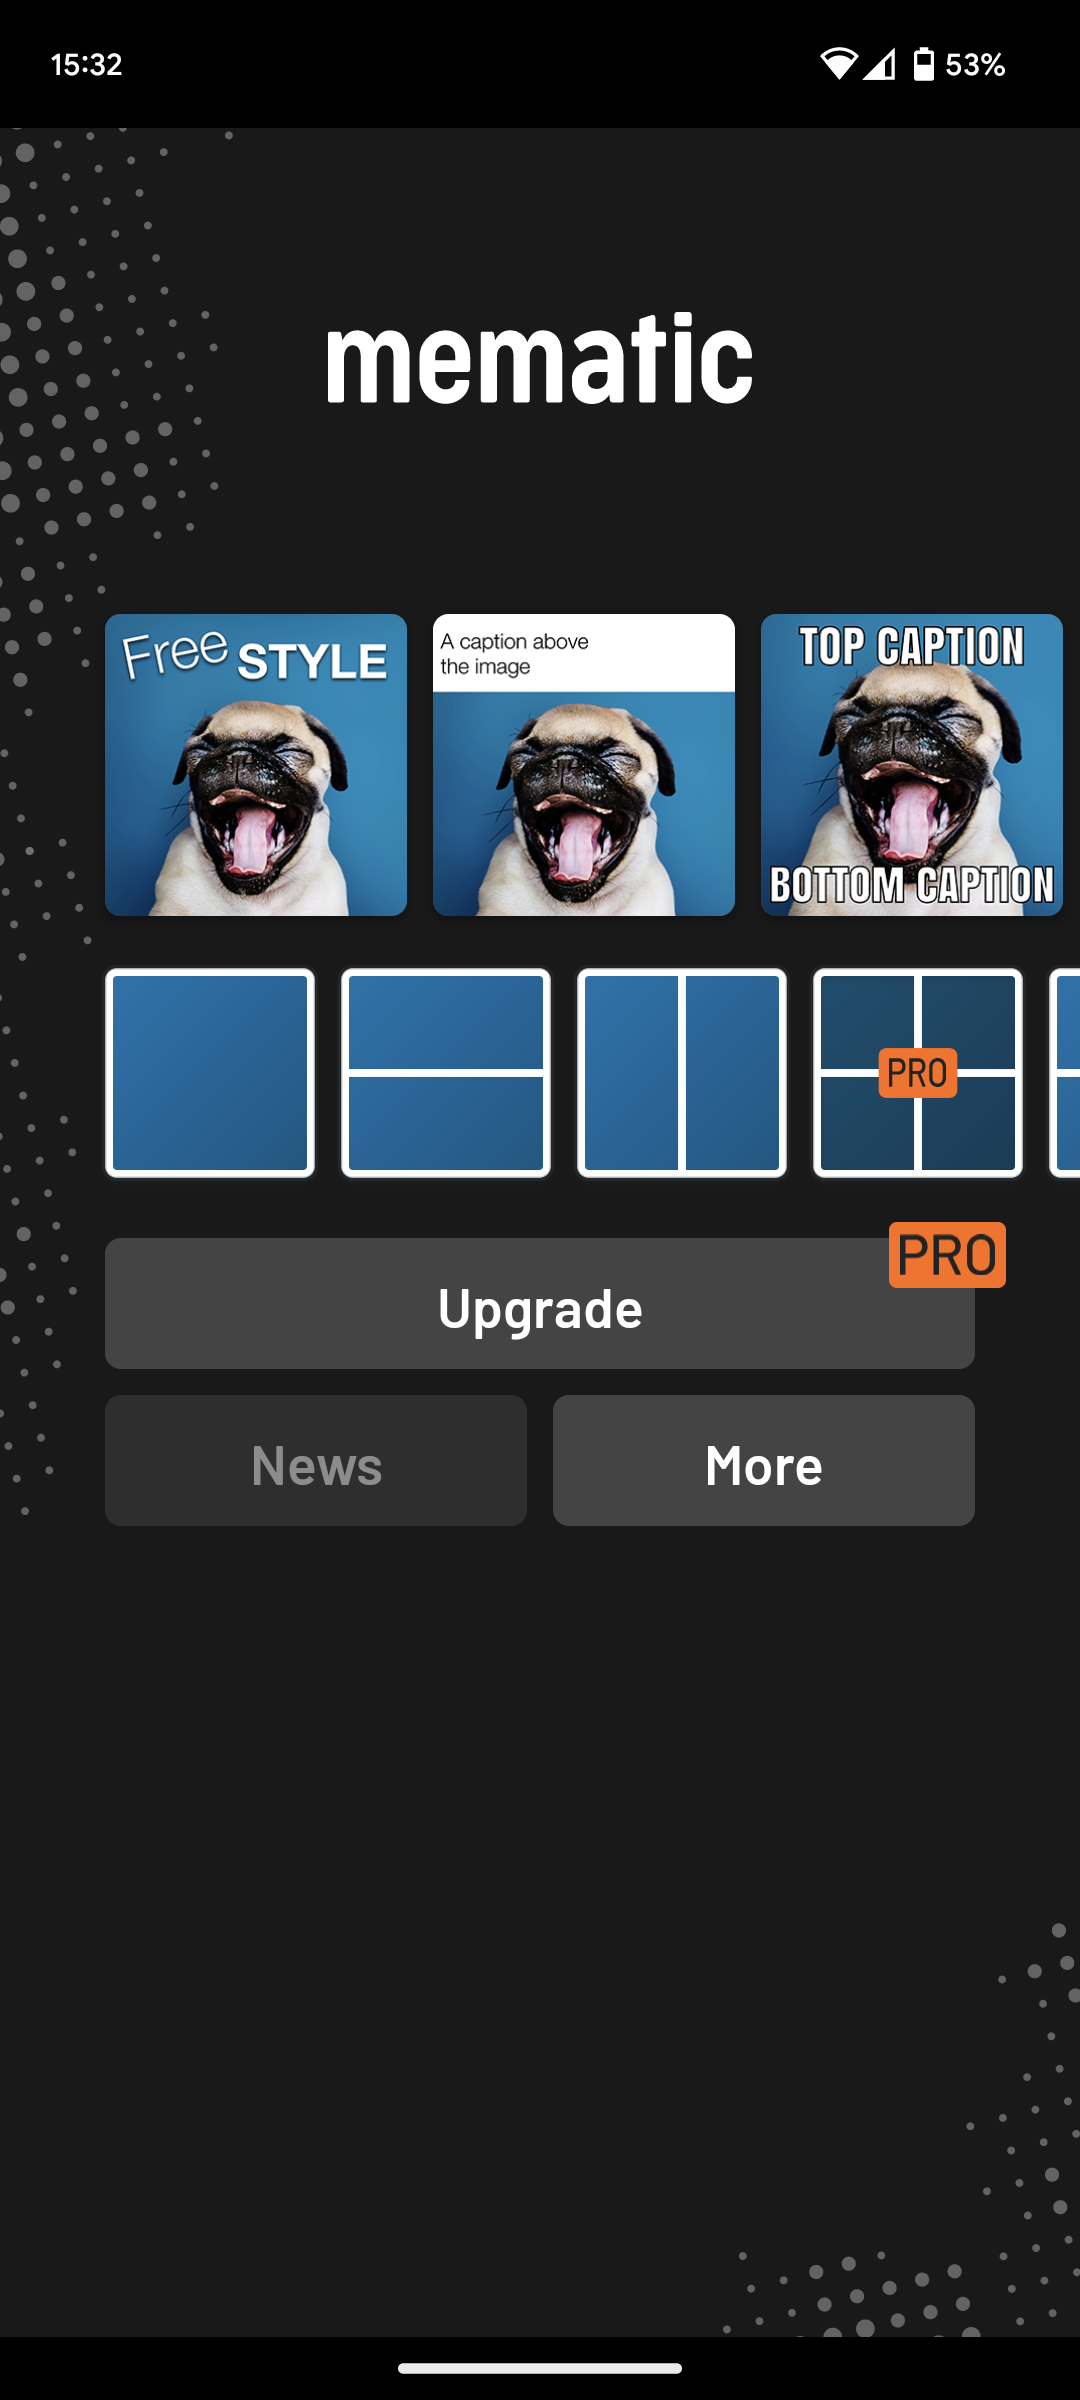
\includegraphics[width=\linewidth]{text/img/mematic/initial-screen.png}
        \caption{Initial screen of the Mematic application}
        \label{fig:mematic-initial}
    \end{subfigure}
    \begin{subfigure}{0.3\textwidth}
        \centering
        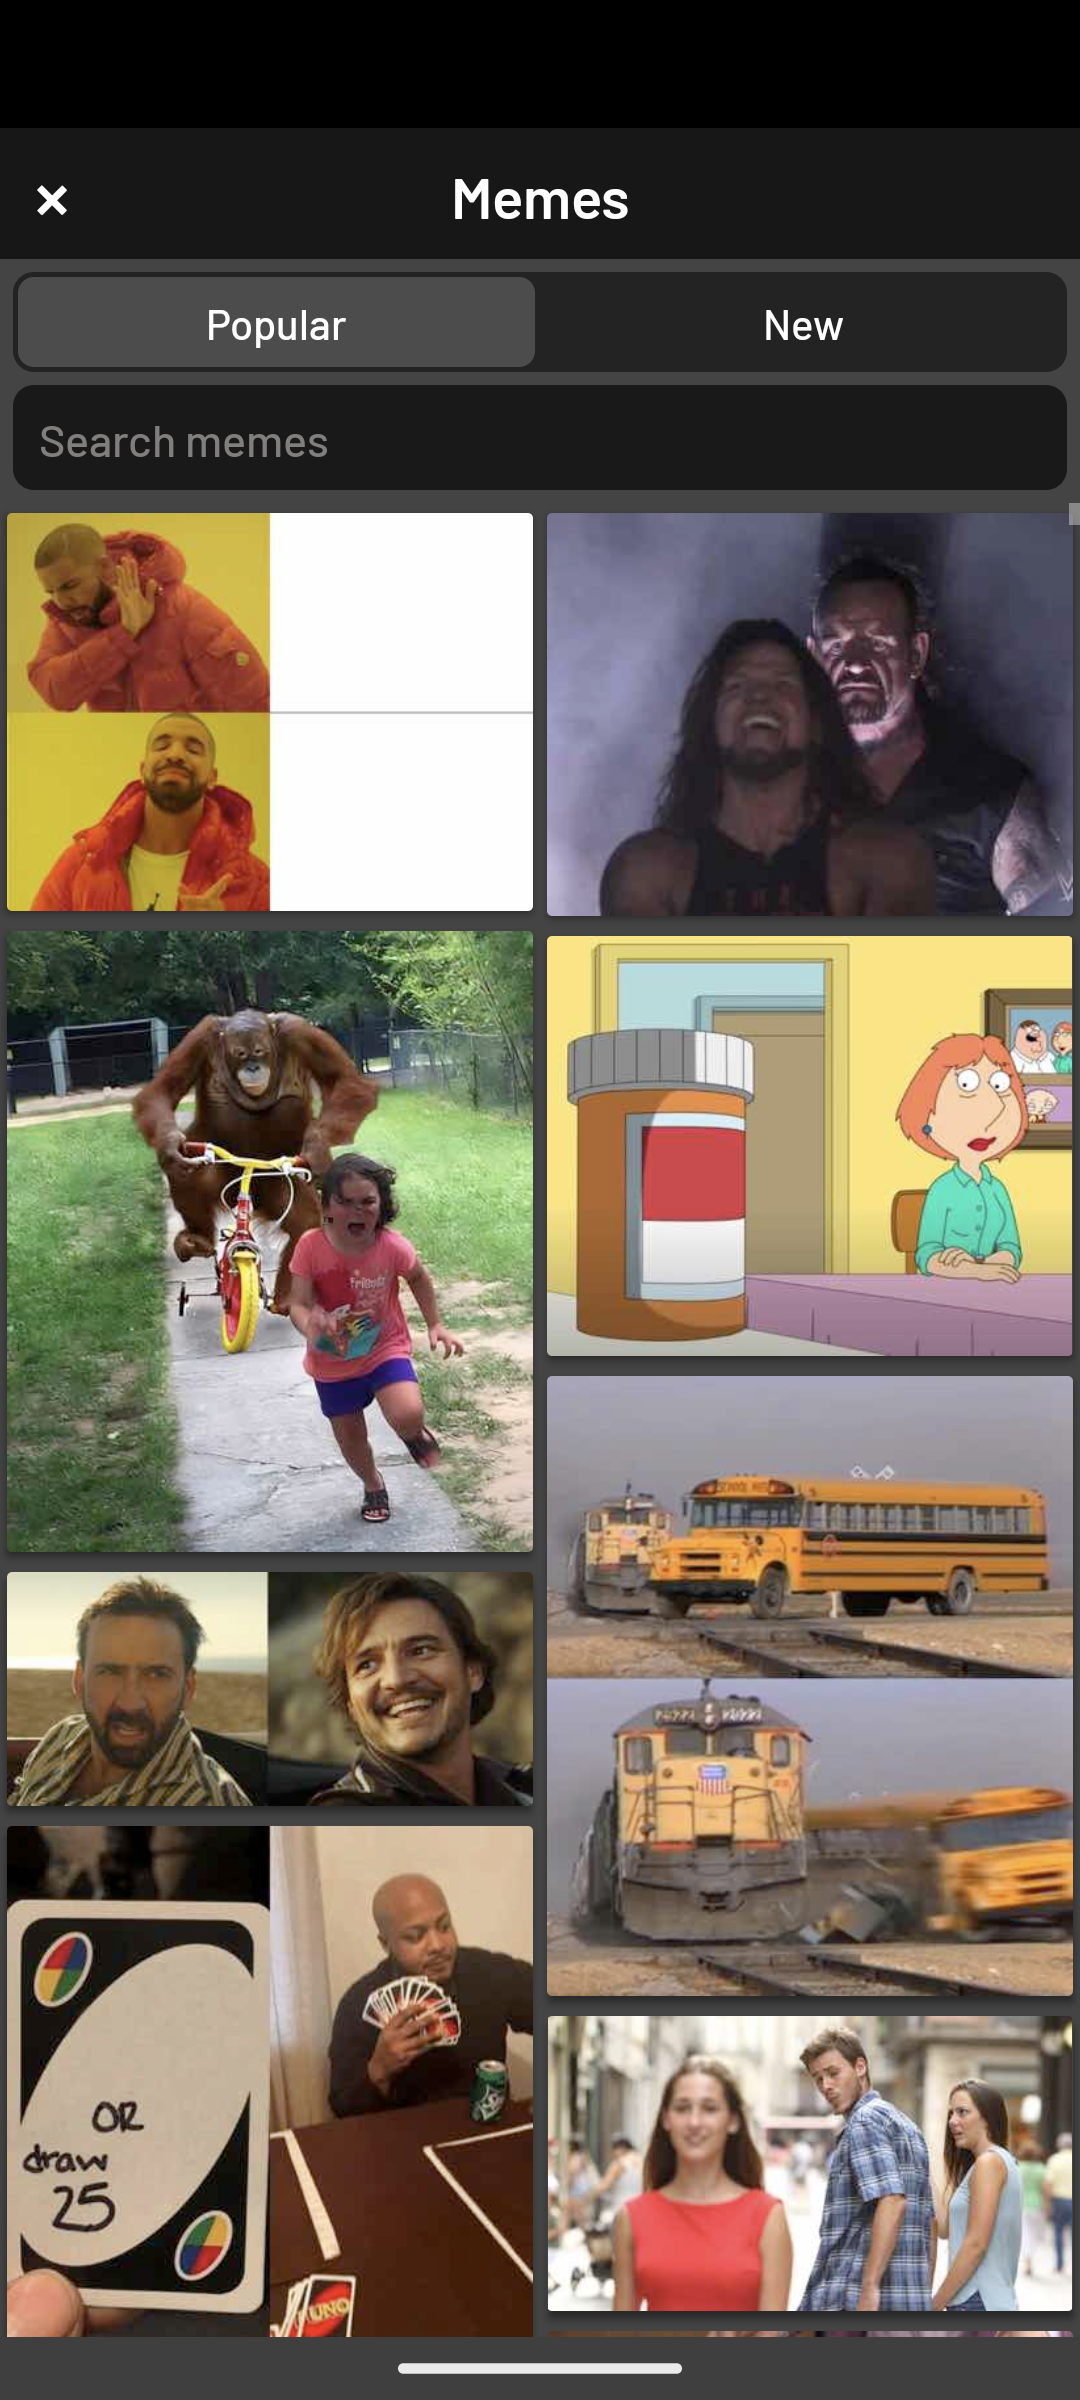
\includegraphics[width=\linewidth]{text/img/mematic/template-select.png}
        \caption{The template selection screen.}
        \label{fig:mematic-template-selection}
    \end{subfigure}
    \begin{subfigure}{0.3\textwidth}
        \centering
        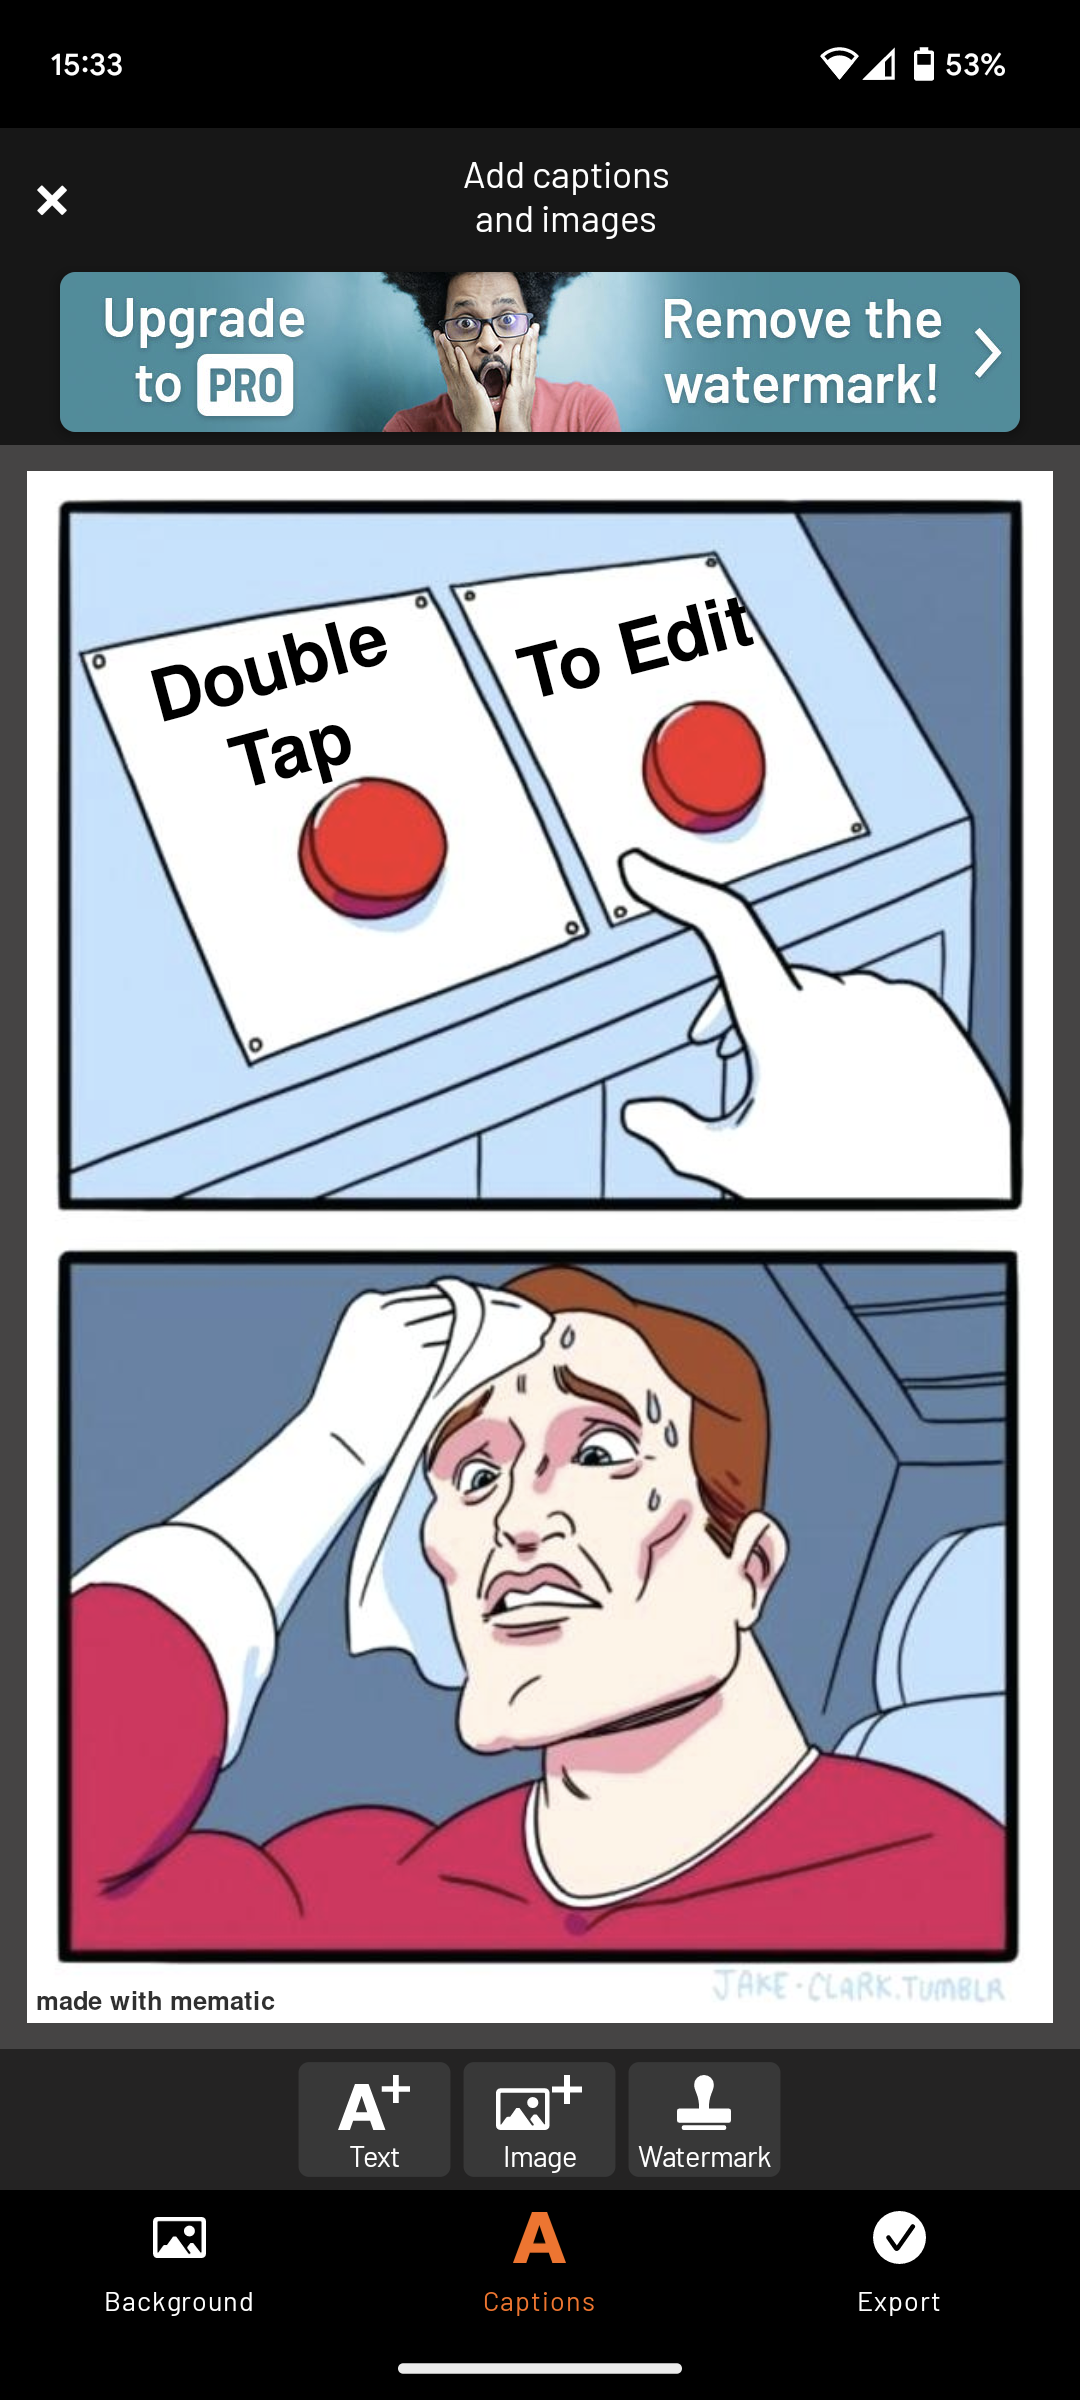
\includegraphics[width=\linewidth]{text/img/mematic/meme-edit.png}
        \caption{The meme edit screen.}
        \label{fig:mematic-meme-edit}
    \end{subfigure}
    % \end{figure}
    % \begin{figure}\ContinuedFloat
    \begin{subfigure}{0.3\textwidth}
        \centering
        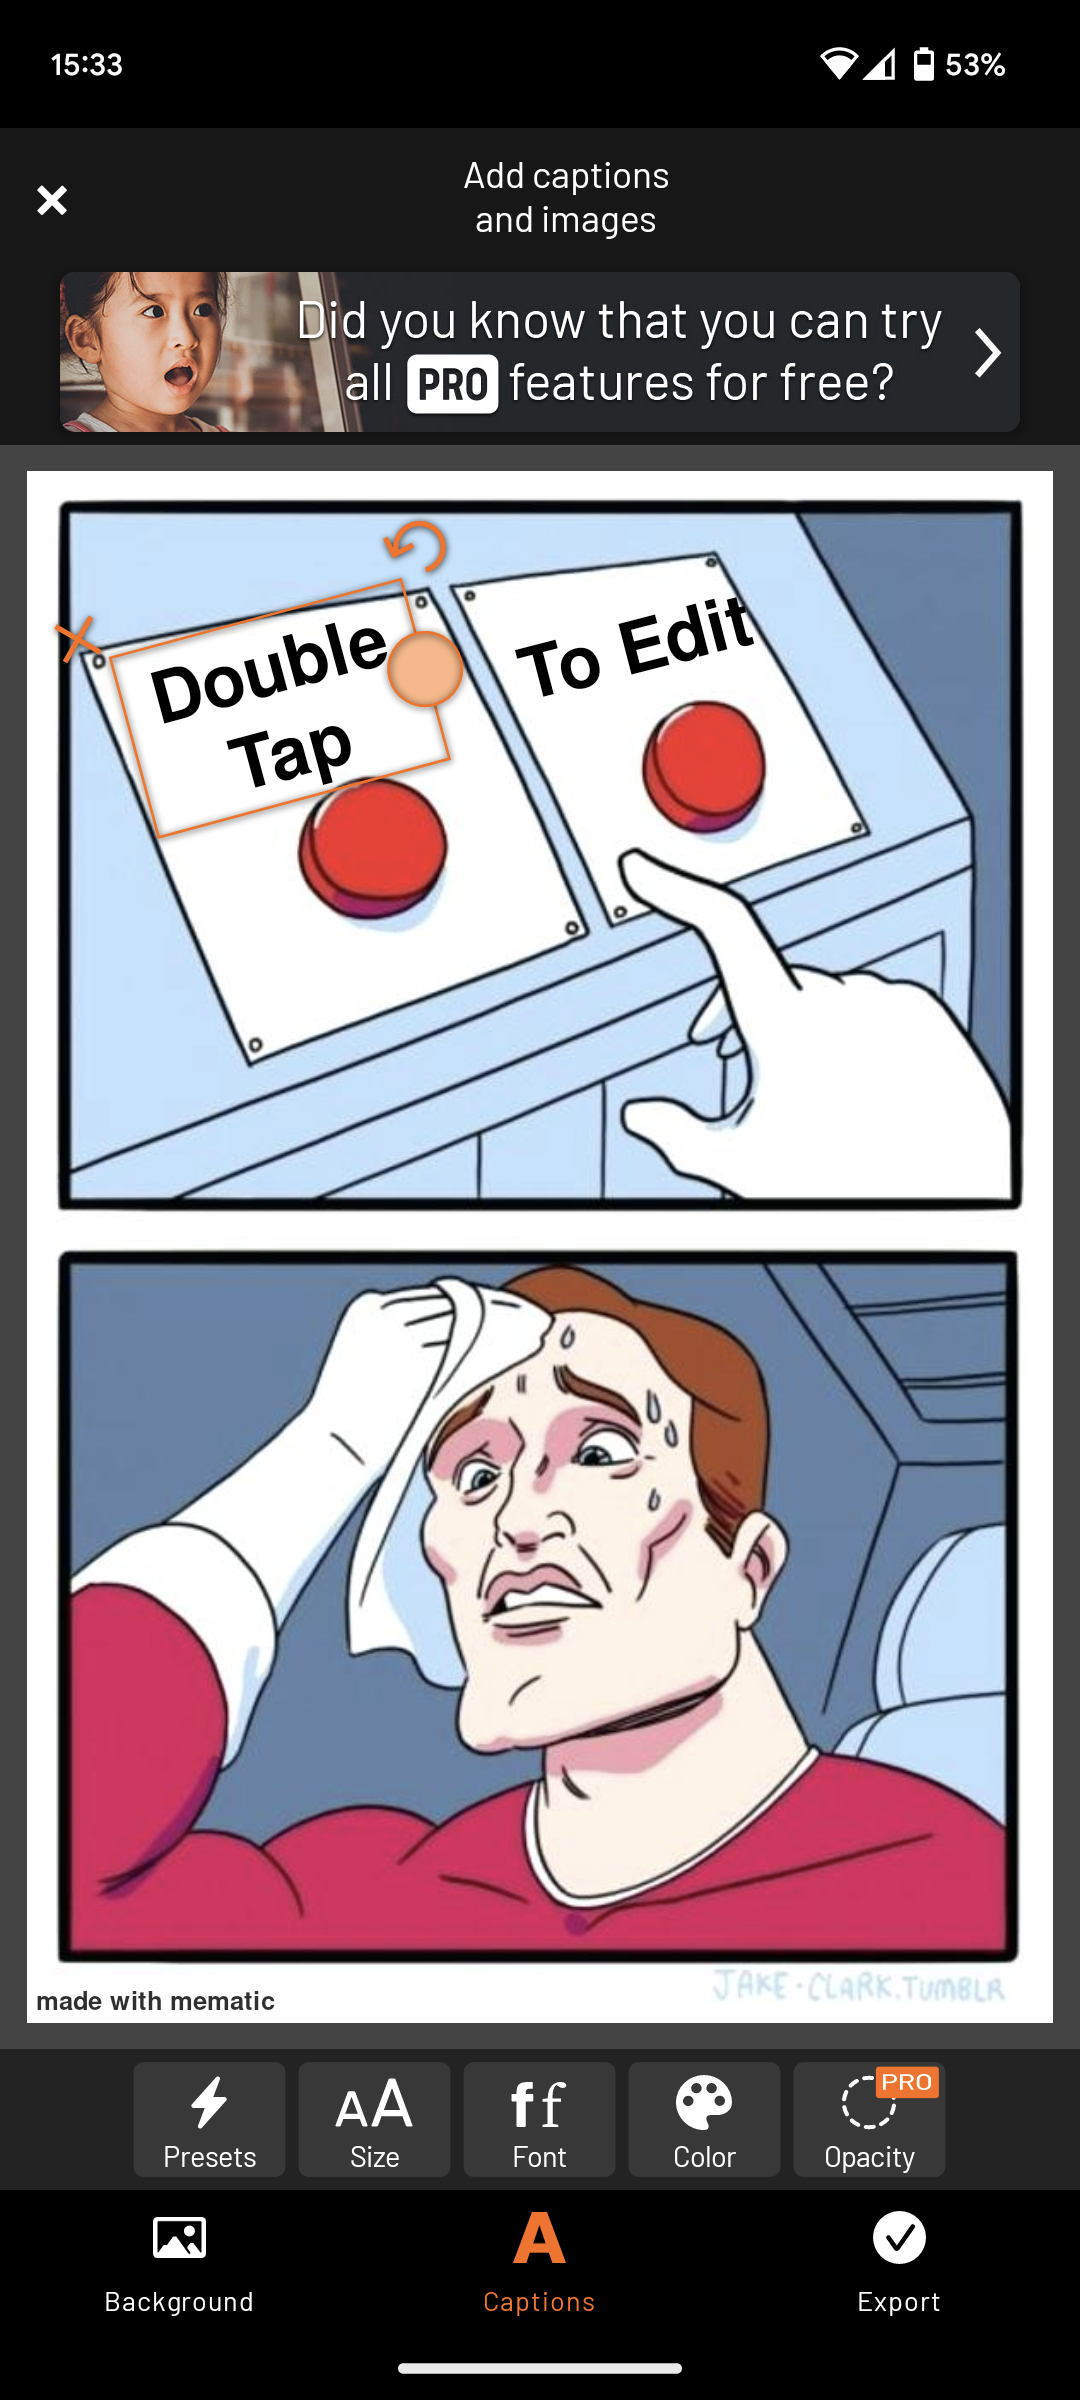
\includegraphics[width=\linewidth]{text/img/mematic/text-edit.png}
        \caption{The text editing controls.}
        \label{fig:mematic-text-edit}
    \end{subfigure}
    \begin{subfigure}{0.3\textwidth}
        \centering
        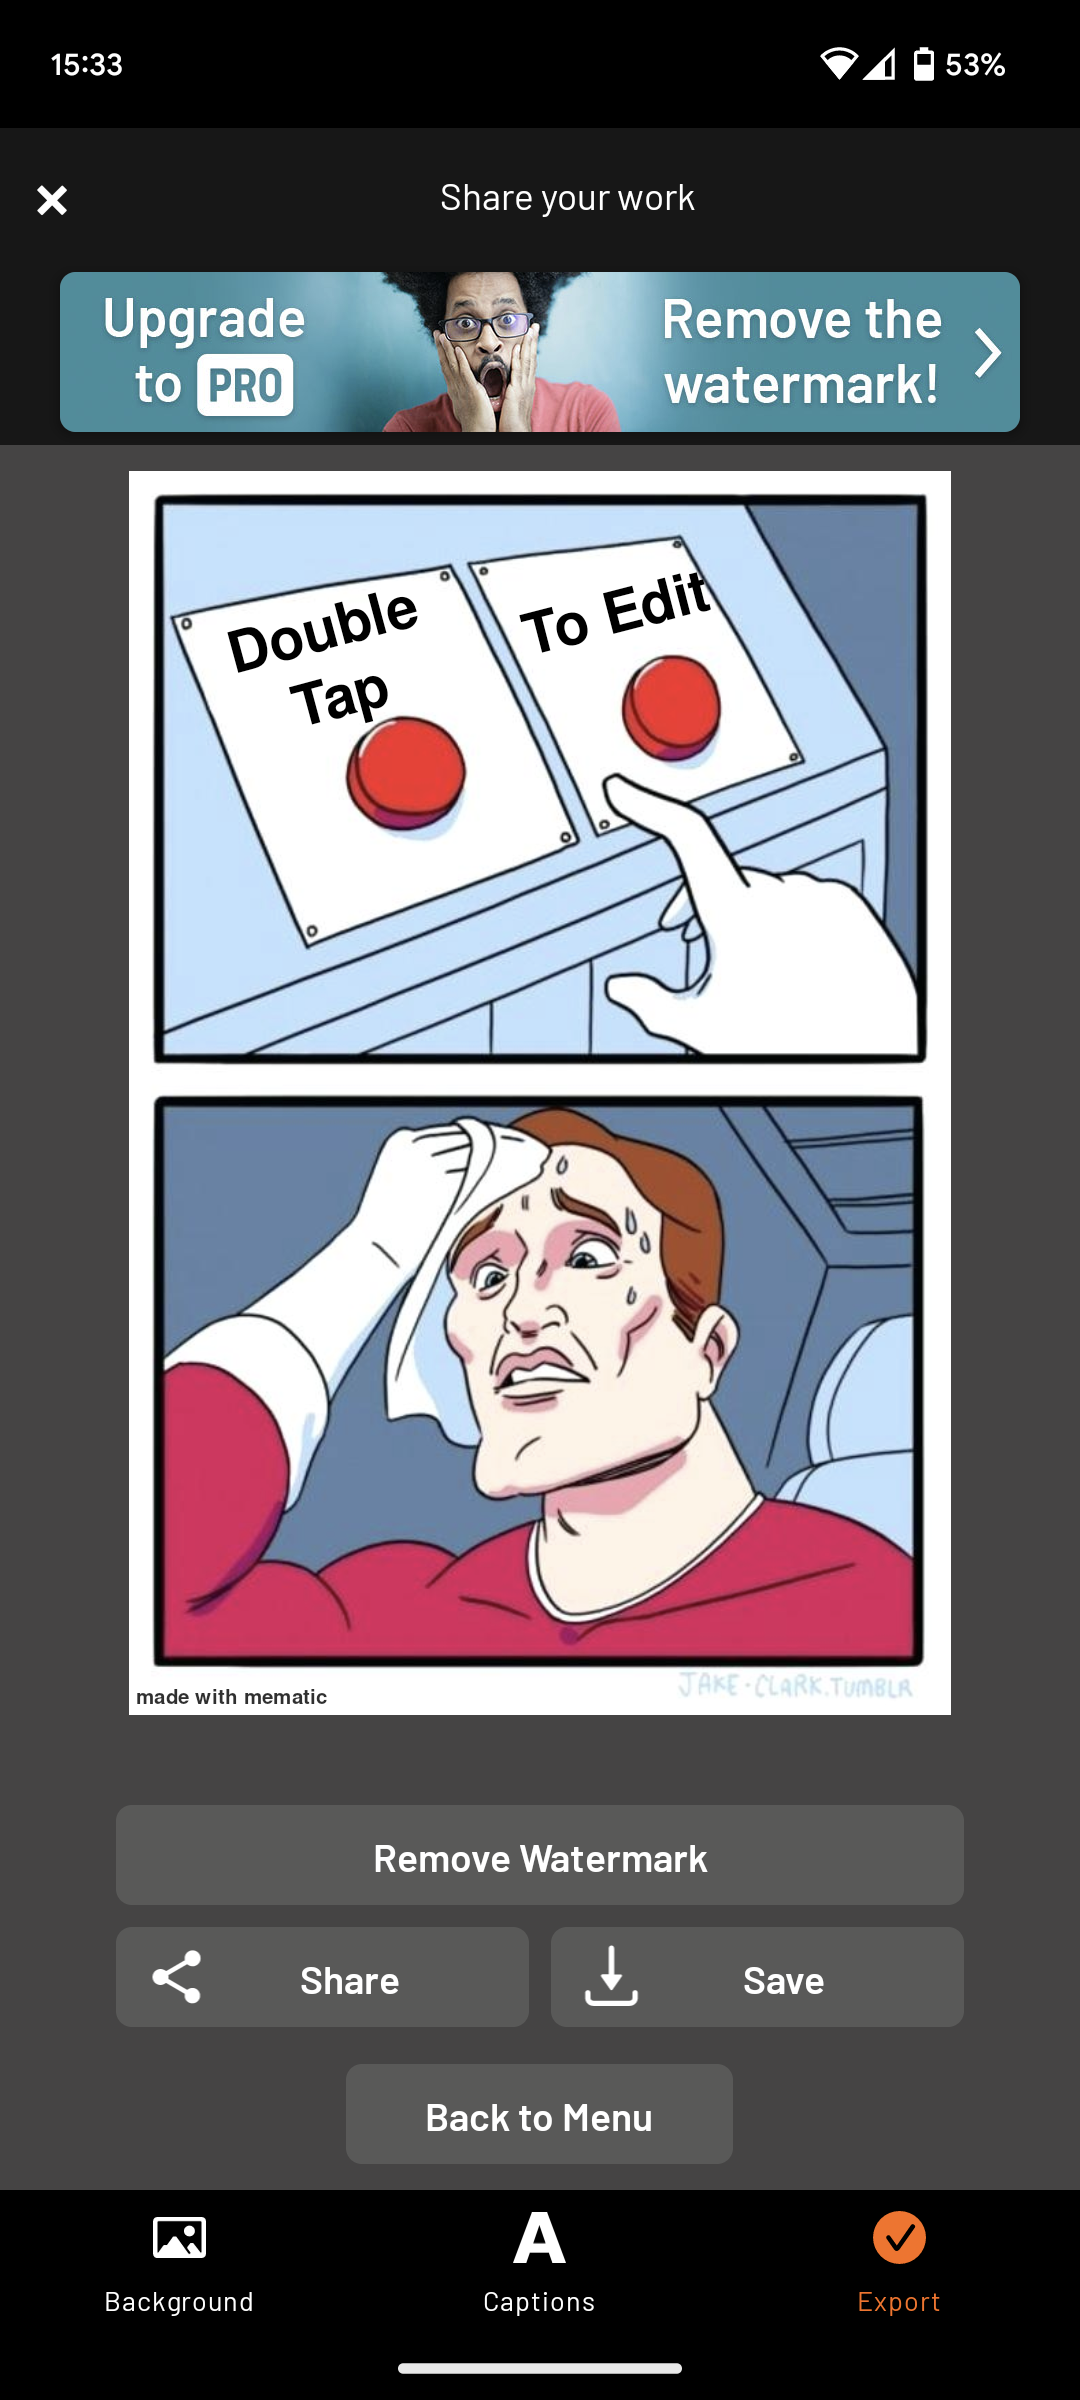
\includegraphics[width=\linewidth]{text/img/mematic/export.png}
        \caption{Exporting a meme.}
        \label{fig:mematic-export}
    \end{subfigure}
    \caption{Screenshots of Mematic}
    \label{fig:mematic}
\end{figure}

%%%%%%%%%%%%%%%%%%%%%%%%%%%%%%%%%%%%%%%%%%%%%%%
\section{Use Case Analysis}
%%%%%%%%%%%%%%%%%%%%%%%%%%%%%%%%%%%%%%%%%%%%%%%

This section of the thesis provides detailed use cases of the application. A use case describes a sequence of interactions between a system and an external actor that results in the actor being able to achieve some outcome of value.\cite{software-requirements}

\subsection{Actors}

\paragraph*{New User} is a user that has landed on the application but hasn't registered. Such a user has a very limited experience in the application.

\paragraph*{Authenticated user} is a user that has completed the registration process and thus has access to the whole application including all the features restricted for registered users.

\subsection{Use Cases}

Overview of all the use cases is shown in the figure \ref{fig:use-case}. All the use cases are described in detail in the following table.

\begin{figure}
    \centering
    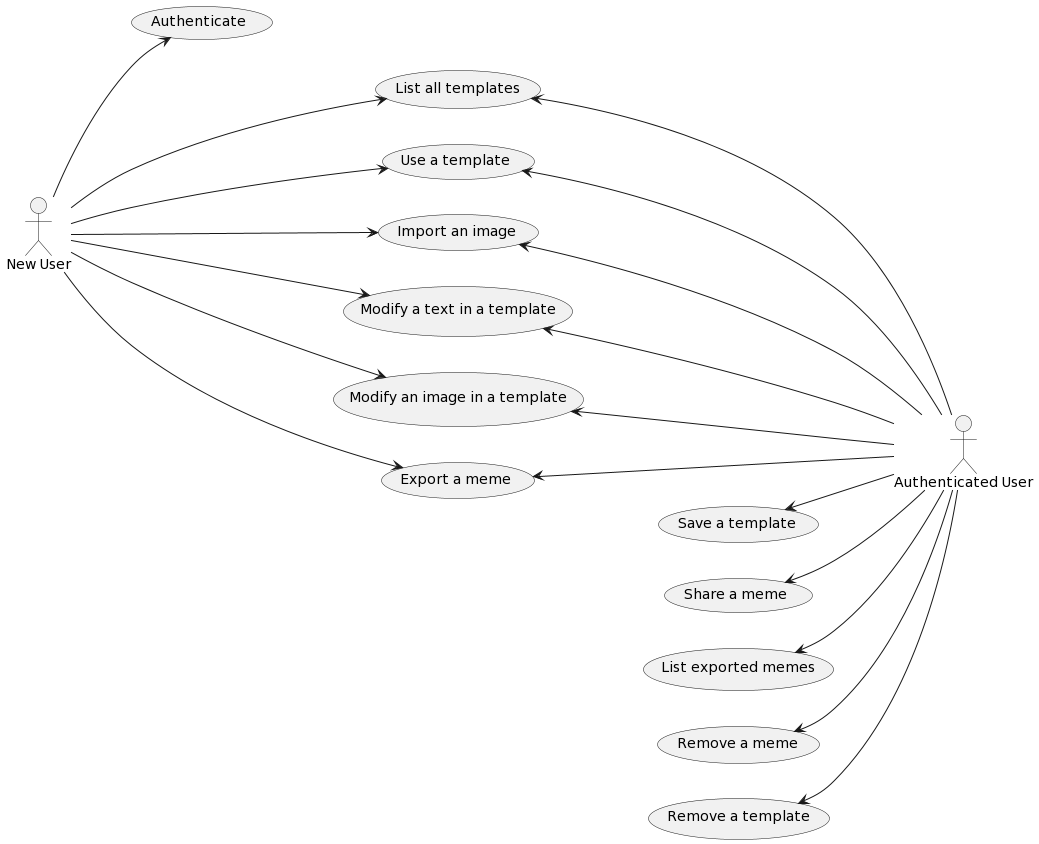
\includegraphics[width=\textwidth]{text/diagram/use-case.png}
    \caption{Use Case Diagram.}
    \label{fig:use-case}
\end{figure}

% \raggedright\arraybackslash
\renewcommand{\arraystretch}{1.8}

\newenvironment{usecaseenum}[1][]
{
    \vspace{-0.5\baselineskip}
    \begin{enumerate}[#1,noitemsep,topsep=0pt,partopsep=0pt,parsep=0pt,after=\vspace{-\baselineskip},align=left,widest*=1,labelsep=1pt]
        }
        {
    \end{enumerate}
}

\noindent
\begin{longtable}{@{}>{\raggedright\arraybackslash}p{3cm} p{11cm}}
    \hline
    \multicolumn{2}{c}{\textbf{Authenticate}}
    \\
    \hline

    \textbf{Actors}         & New User
    \\

    \textbf{Description}    & The New User expects to be able to authenticate into the application by providing valid credentials. There are two possible ways of authenticating, either by using an email address or by using an external identity provider.
    \\

    \textbf{Preconditions}  & The user has a valid email address, or they are registered with one of the valid external identity providers.
    \\

    \textbf{Normal Flow}    & \begin{usecaseenum}
                                  \item Click the login button.
                                  \item Fill out an email in the respective form field.
                                  \item Click the \texttt{Sign in with Email} button.
                                  \item Open the link that the user received on the email address filled out in step 2.
                                  \item The user is authenticated in the newly opened session.
                              \end{usecaseenum}
    \\
    \textbf{Alternate Flow} & \begin{usecaseenum}
                                  \item Click the login button.
                                  \item Click on the identity provider that the user has an account at.
                                  \item Go through the proccess of granting permission to the meme application from the external provider.
                                  \item The user is redirected back to the meme application and is authenticated.
                              \end{usecaseenum}
    \\

    \textbf{Postconditions} & \begin{usecaseenum}
                                  \item The user is authenticated.
                                  \item User information is stored in the database.
                              \end{usecaseenum}
    \\
    \hline
    \multicolumn{2}{c}{\textbf{List all templates}}
    \\
    \hline

    \textbf{Actors}         & New User, Authenticated User
    \\

    \textbf{Description}    & The user expects to be able to list all the templates created by them and all the templates by other users which are publicly available.
    \\

    \textbf{Preconditions}  & There are any available templates created by the user\newline or there are any publicly available templates.
    \\

    \textbf{Normal Flow}    & Visit the page that lists all templates.
    \\

    \textbf{Postconditions} & User can browse all the templates available to them.
    \\
    \hline
    \multicolumn{2}{c}{\textbf{Use a template}}
    \\
    \hline

    \textbf{Actors}         &  New User, Authenticated User
    \\

    \textbf{Description}    & The user expects to be able to use an available template to create a meme.
    \\

    \textbf{Preconditions}  & There is at least one available template.
    \\

    \textbf{Normal Flow}    & Click on a template on the create page.
    \\

    \textbf{Alternate Flow}    & Click on a template on the list templates page.
    \\

    \textbf{Postconditions} & User was redirected to the create page and the template is loaded into the editor.
    \\
    \hline
    \multicolumn{2}{c}{\textbf{Import an image}}
    \\
    \hline

    \textbf{Actors}         & New User, Authenticated User
    \\

    \textbf{Description}    & The user expects to be able to import an image either from their local device or the internet, or alternatively, utilize the integrated text-to-image AI functionality for image generation.
    \\

    \textbf{Preconditions}  & The user has a valid image file on their device,\newline or they have a valid \acrshort{url} to an image,\newline or they have a valid text to generate an image from.
    \\

    \textbf{Normal Flow}    & \begin{usecaseenum}
                                  \item Click the \texttt{Add image} button.
                                  \item[\textcolor{enumgray}{\bfseries{2a.}}] Click the upload button and select the image file.
                                  \item[\textcolor{enumgray}{\bfseries{2b.}}] Paste the \acrshort{url} to the image and click the \texttt{Use} button.
                                  \item[\textcolor{enumgray}{\bfseries{2c.}}] Paste the text to generate an image from and click the \texttt{Generate} button.\setcounter{enumi}{2}
                                  \item Click the \texttt{Next} button.
                                  \item Use the cropping tool to select the part of the image to use.
                                  \item Click the \texttt{Next} button.
                                  \item Click the \texttt{Remove Background} button.
                                  \item[\textcolor{enumgray}{\bfseries{7a.}}] Click the \texttt{Use original image} button.
                                  \item[\textcolor{enumgray}{\bfseries{7b.}}] Click the \texttt{Use image without background} button.
                              \end{usecaseenum}
    \\

    \textbf{Postconditions} & The image is imported and can be used in the application.
    \\
    \hline
    \multicolumn{2}{c}{\textbf{Modify a text in a template}}
    \\
    \hline

    \textbf{Actors}         & New User, Authenticated User
    \\

    \textbf{Description}    & The user expects the ability to change the contents and the properties of a text
    \\

    \textbf{Preconditions}  & \begin{usecaseenum}
                                  \item The user is editing a template.
                                  \item The template has a text element in it.
                              \end{usecaseenum}
    \\

    \textbf{Normal Flow}    & \begin{usecaseenum}
                                  \item Click and drag the text's corners to resize it.
                                  \item Click and drag the control point above the text to rotate it.
                                  \item Click and drag the text to move it.
                                  \item Use the input field to change the content.
                                  \item Click on the colors in the text properties to change the outline and fill colors of the text.
                                  \item Click on the settings icon to open the text properties dialog.
                                  \item Change the text's size in the properties dialog.
                              \end{usecaseenum}
    \\
    \textbf{Postconditions} & The text is modified.
    \\
    \hline
    \multicolumn{2}{c}{\textbf{Modify an image in a template}}
    \\
    \hline

    \textbf{Actors}         & New User, Authenticated User
    \\

    \textbf{Description}    & The user expects the ability to change how the image is displayed in the template.
    \\

    \textbf{Preconditions}  & \begin{usecaseenum}
                                  \item The user is editing a template.
                                  \item The template has a text element in it.
                              \end{usecaseenum}
    \\

    \textbf{Normal Flow}    & \begin{usecaseenum}
                                  \item Click and drag the image's corners to resize it.
                                  \item Click and drag the control point above the image to rotate it.
                                  \item Click and drag the image to move it.
                              \end{usecaseenum}
    \\

    \textbf{Postconditions} & The image is modified.
    \\
    
    \hline
    \multicolumn{2}{c}{\textbf{Exporte a meme}}
    \\
    \hline

    \textbf{Actors}         &  New User, Authenticated User
    \\

    \textbf{Description}    & The user expects to be able to export a meme and download it.
    \\

    \textbf{Preconditions}  & The user has a template loaded into the editor.
    \\

    \textbf{Normal Flow}    & Click on the \texttt{Export Meme} button.
    \\

    \textbf{Postconditions} & The meme is exported and a dialog with the image is shown.
    \\

    \hline
    \multicolumn{2}{c}{\textbf{Save a template}}
    \\
    \hline

    \textbf{Actors}         &  Authenticated User
    \\

    \textbf{Description}    & The user expects to be able to save an edited template.
    \\

    \textbf{Preconditions}  & The user has a template loaded into the editor.
    \\

    \textbf{Normal Flow}    & \begin{usecaseenum}
        \item Click on the \texttt{Save Template} button.
        \item Edit the template's name.
        \item Set the template's visibility.
        \item Click on the \texttt{Save} button. 
    \end{usecaseenum}
    \\

    \textbf{Postconditions} & The template is saved and can be used in the future.
    \\

    \hline
    \multicolumn{2}{c}{\textbf{Share a meme}}
    \\
    \hline

    \textbf{Actors}         &  Authenticated User
    \\

    \textbf{Description}    & The user expects to be able to get a sharable \acrshort{url} to the meme.
    \\

    \textbf{Preconditions}  & The user has exported a meme and the dialog with the image is shown.
    \\

    \textbf{Normal Flow}    & \begin{usecaseenum}
        \item Click on the \texttt{Copy} button.
    \end{usecaseenum}
    \\

    \textbf{Postconditions} & The \acrshort{url} to the meme is copied to the clipboard.
    \\

    \hline
    \multicolumn{2}{c}{\textbf{List exported memes}}
    \\
    \hline

    \textbf{Actors}         & Authenticated User
    \\

    \textbf{Description}    & The user expects to be able to list all the memes exported by them.
    \\

    \textbf{Preconditions}  & The user has exported at least one meme and has not deleted it.
    \\

    \textbf{Normal Flow}    & Visit the page that lists users memes.
    \\

    \textbf{Postconditions} & User can view all the memes that they have exported.
    \\
    \textbf{Postconditions} & The template is saved and can be used in the future.
    \\

    \hline
    \multicolumn{2}{c}{\textbf{Remove a meme}}
    \\
    \hline

    \textbf{Actors}         &  Authenticated User
    \\

    \textbf{Description}    & The user expects to be able to remove a meme.
    \\

    \textbf{Preconditions}  & The user has exported at least one meme and has not deleted it. The user is on the page that lists all the memes exported by them.
    \\

    \textbf{Normal Flow}    & \begin{usecaseenum}
        \item Click on the \texttt{Delete Meme} button.
    \end{usecaseenum}
    \\

    \textbf{Postconditions} & The meme is deleted.
    \\
    \hline
    \multicolumn{2}{c}{\textbf{Remove a template}}
    \\
    \hline

    \textbf{Actors}         &  Authenticated User
    \\

    \textbf{Description}    & The user expects to be able to remove a template.
    \\

    \textbf{Preconditions}  & The user has saved at least one template and has not deleted it. The user is on the page that lists all the templates they have saved.
    \\

    \textbf{Normal Flow}    & \begin{usecaseenum}
        \item Click on the \texttt{Delete Template} button.
    \end{usecaseenum}
    \\

    \textbf{Postconditions} & The template is deleted.
    \\
\end{longtable}

% Authenticate
% List all templates
% Use a template
% Import an image
% Modify a text in a template
% Modify an image in a template
% Export a meme
% Save a template
% Share a meme
% Remove a meme
% Remove a template


%%%%%%%%%%%%%%%%%%%%%%%%%%%%%%%%%%%%%%%%%%%%%%%
\section{Wireframes}
%%%%%%%%%%%%%%%%%%%%%%%%%%%%%%%%%%%%%%%%%%%%%%%

A wireframe is the basic blueprint that illustrates the core form and function found on a single screen of your web page or application \cite{wireframing}. The wireframes do not exactly resemble the finished product, but they provide an insight into the basic functionalities and structure of the application. All of the individual pages of the application are featured in the figure \ref{fig:wireframes} and the import image dialog is shown in the figure \ref{fig:wireframes-import-dialog}.

\subsection{Create Page}

The \texttt{Create Page} is the main page of the application where the user lands at. The wireframes show it in two versions, one where a user has logged in to the application (image \ref{fig:wireframes-create-logged}) and one where the user is anonymous (image \ref{fig:wireframes-create-anonymous}).

The main part of the page is mostly the same for both types of users. The top part of the page is used to get a base template, which can either be selected from the list of available templates or imported from an image.

To the left is the graphical section. It features a canvas where the user can see the template, the texts and the added images. The user can move the texts and images around, rotate them and resize them. The user can also add new texts and images to the canvas, where the images would be imported using the import image dialog (see \autoref{sec:import-image-dialog}).

To the right is the properties section of the page. It displays a list of all the texts and images that are currently on the canvas. The user can use this section to modify the content of each individual text and it's the outline and fill colors. The order in which the texts and images are displayed in the properties section is the same as the order in which they are displayed in the graphical section. Texts and images can be moved up and down in the list using the arrows on the left side of each item. The user can also remove texts and images from the canvas using the \texttt{Remove} button on the right side of each item.

The bottom of the right section is dedicated to saving the template and exporting a meme image. Only logged-in users can save the template, but both types of users can export a meme image.

\subsection{All Templates Page}

The \texttt{All Templates} page shows all the available templates that the user can modify and use them to generate memes. If the user is logged in, the page will show all the user's templates and all the public templates from other users. If the user is not logged in, the page only shows public templates.

The \texttt{Load More} button is only visible when there are more templates to be loaded. Clicking it will load more templates.

Clicking any of the displayed templates redirects the user to the \texttt{Create page} and loads the clicked template into the editor.

\subsection{My Templates Page}

The \texttt{My Templates Page} is only available to logged-in users. Here, the users can view all the templates they created and saved. There are two options for each template, opening it in the \texttt{Create Page}, or deleting it.

\subsection{My Memes Page}

The \texttt{My Memes Page} has a similar design to the \texttt{My Templates Page}, but instead of a list of templates, it shows a list of memes. There is an option to open the meme's details, which would show a larger version of the image and the link to the meme's image.

\subsection{Profile Page}

\texttt{Profile Page} shows the user's statistics and information. There is a section with the user's information, like their name, email, and profile image. There is also a section with the user's statistics, like the number of templates and memes they created. The user is able to change their profile image by clicking on icon in the top left corner the image and selecting a new one. They can also change their username using the form below the statistics.

\begin{figure}
    \centering
    \begin{subfigure}{0.45\textwidth}
        \centering
        \fbox{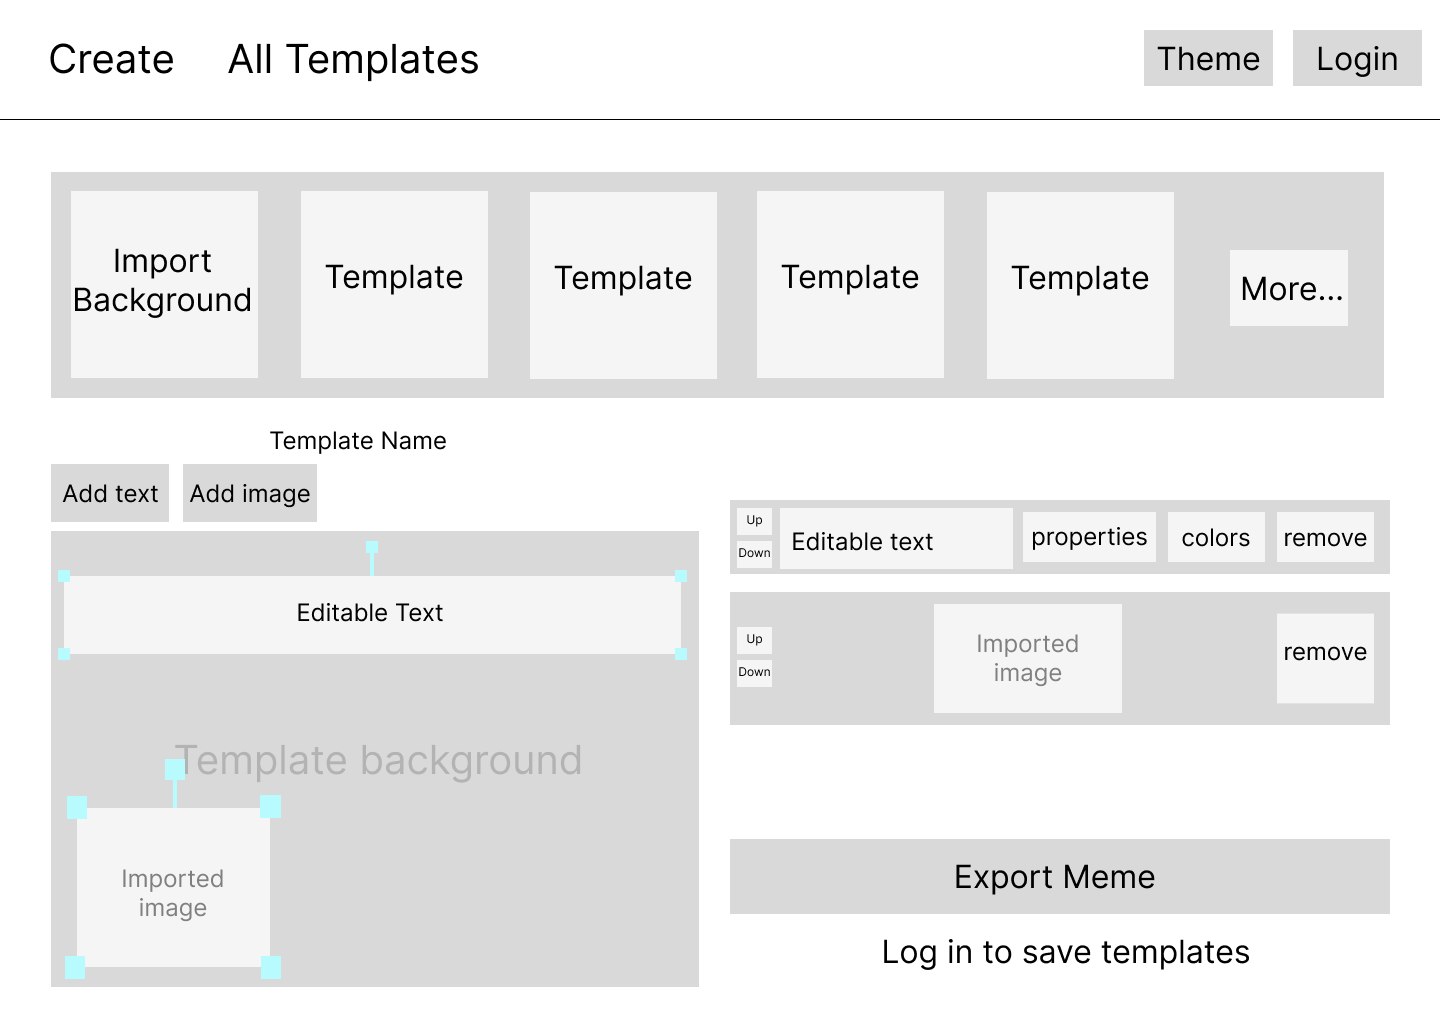
\includegraphics[width=\textwidth]{text/img/wireframes/Create Anonymous.png}}
        \caption{Create page, anonymous user.}
        \label{fig:wireframes-create-anonymous}
    \end{subfigure}
    \hspace{1cm}
    \begin{subfigure}{0.45\textwidth}
        \centering
        \fbox{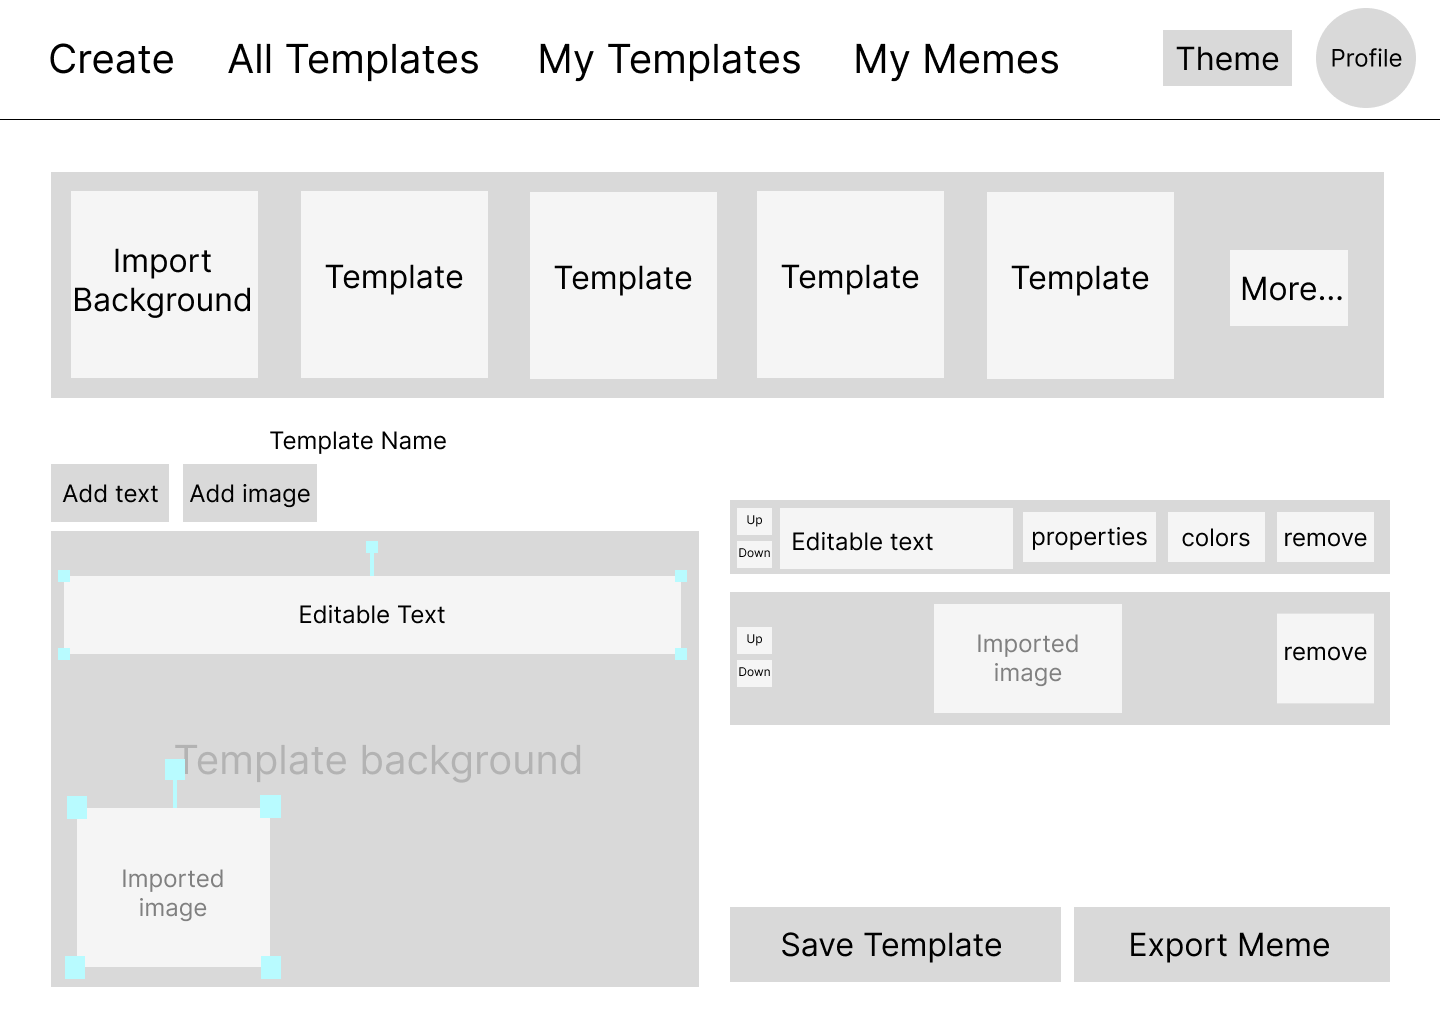
\includegraphics[width=\linewidth]{text/img/wireframes/Create Logged.png}}
        \caption{Create page, logged-in user.}
        \label{fig:wireframes-create-logged}
    \end{subfigure}
    \begin{subfigure}{0.45\textwidth}
        \centering
        \fbox{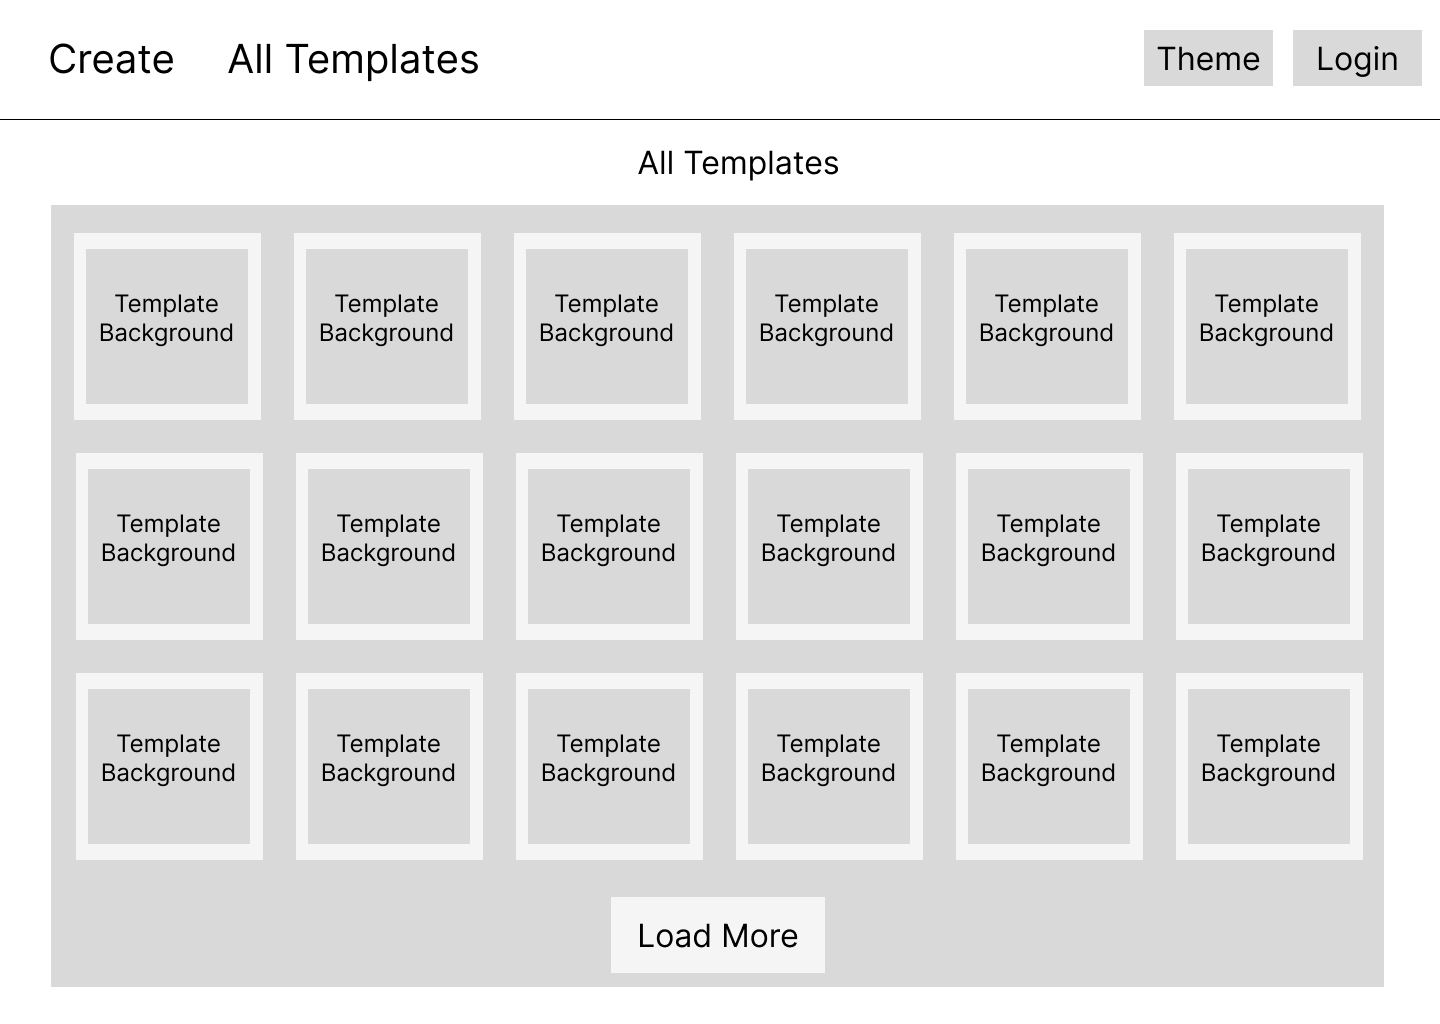
\includegraphics[width=\linewidth]{text/img/wireframes/All Templates.png}}
        \caption{All templates page.}
        \label{fig:wireframes-all-templates}
    \end{subfigure}
    \hspace{1cm}
    \begin{subfigure}{0.45\textwidth}
        \centering
        \fbox{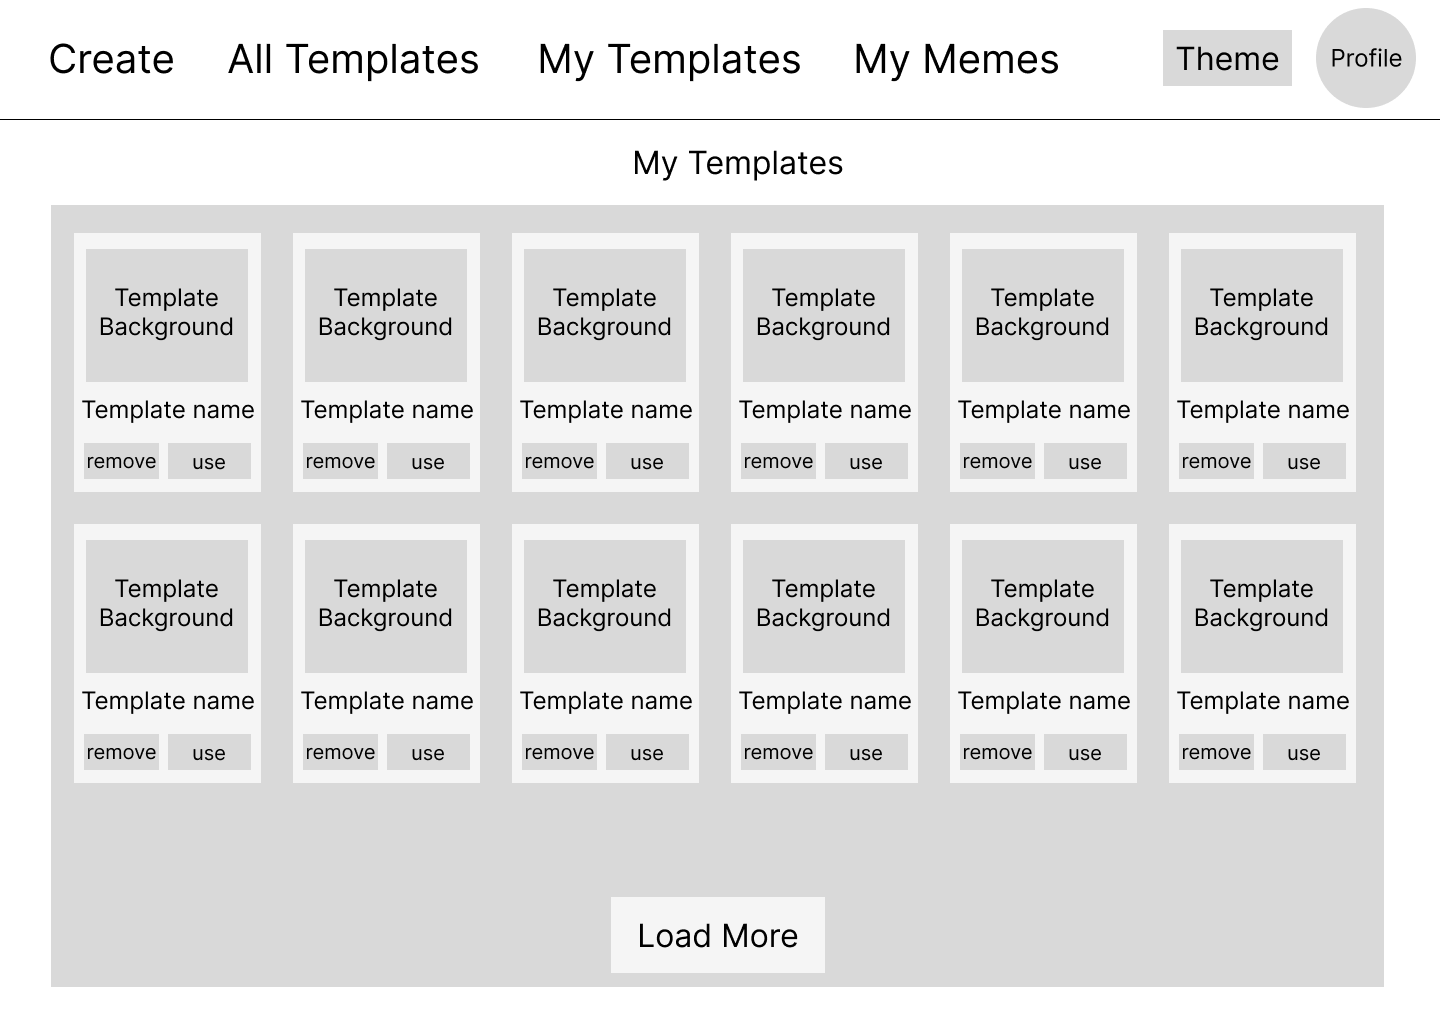
\includegraphics[width=\linewidth]{text/img/wireframes/My templates.png}}
        \caption{My templates page.}
        \label{fig:wireframes-my-templates}
    \end{subfigure}
    \begin{subfigure}{0.45\textwidth}
        \centering
        \fbox{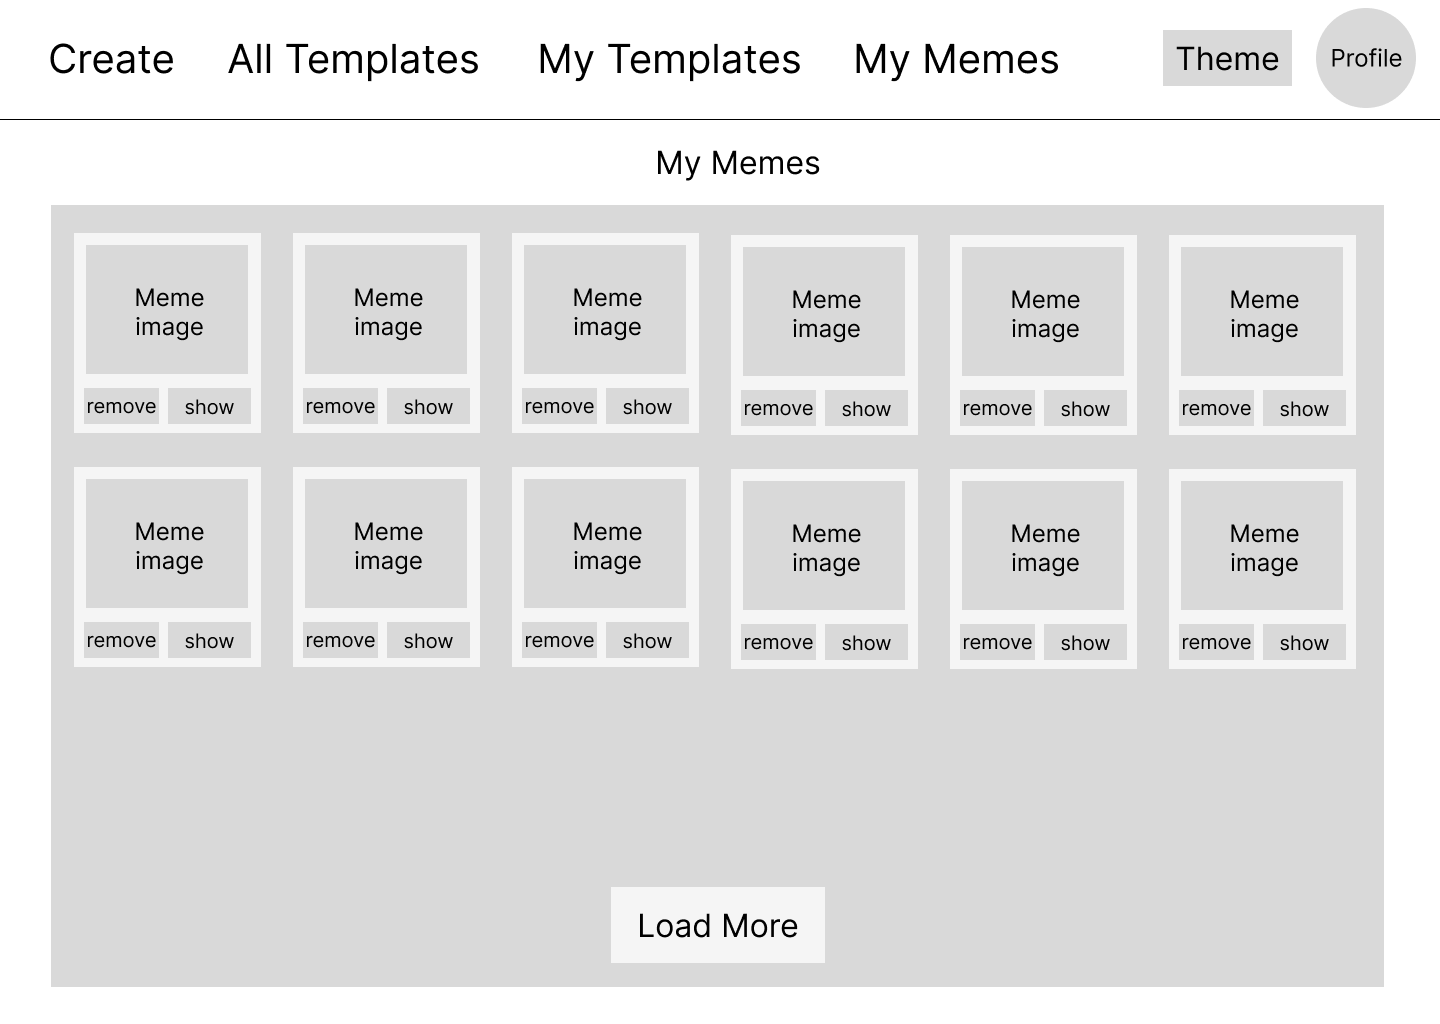
\includegraphics[width=\linewidth]{text/img/wireframes/My memes.png}}
        \caption{My memes page.}
        \label{fig:wireframes-my-memes}
    \end{subfigure}
    \hspace{1cm}
    \begin{subfigure}{0.45\textwidth}
        \centering
        \fbox{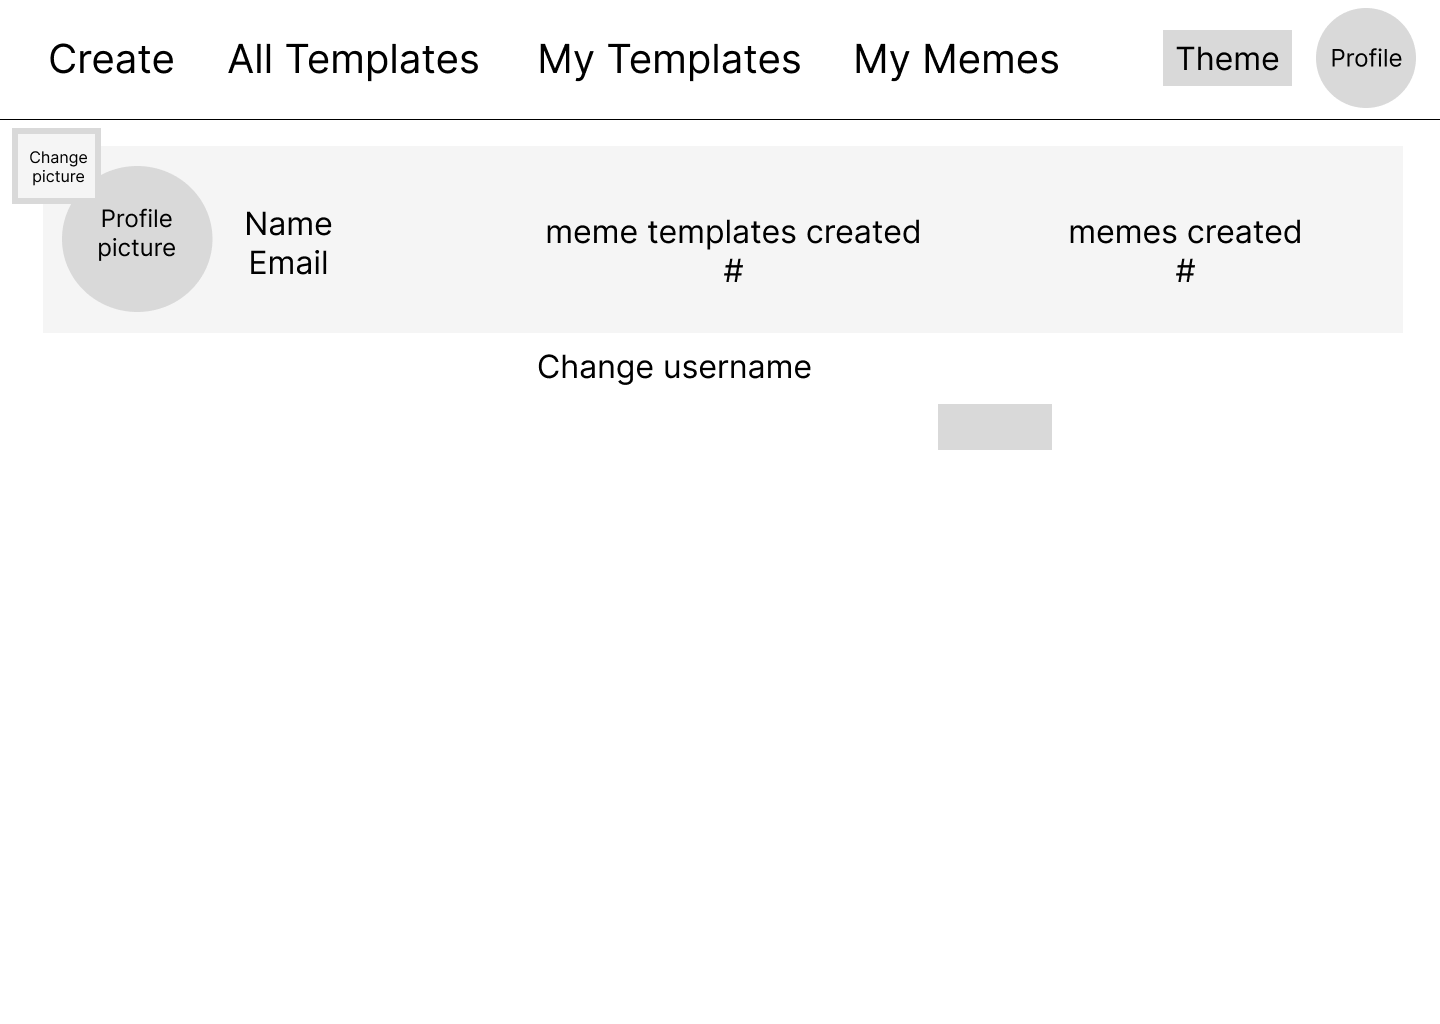
\includegraphics[width=\linewidth]{text/img/wireframes/Profile.png}}
        \caption{Profile page.}
        \label{fig:wireframes-profile}
    \end{subfigure}
    \caption{Wireframes of the application.}
    \label{fig:wireframes}
\end{figure}

\subsection{Import Image Dialog}
\label{sec:import-image-dialog}

The \texttt{Import Image Dialog} is used to import an image to the application, which is used as a template background or is a part of the template. The dialog has three steps.

\paragraph*{Step 1} is used to select the image to import. It is shown on image \ref{fig:wireframes-import-import}. The user can either select an image from their device, paste an \acrshort{url} to an image or paste a text to generate an image from.

\paragraph*{Step 2} is used to crop the image. It is shown on image \ref{fig:wireframes-import-crop}. The user moves the cropping rectangle to select the part of the image to use.

\paragraph*{Step 3} is used to remove the background from the image. If the user doesn't want to remove the background, they can skip this step using the \texttt{Confirm} buttons, which is shown on image \ref{fig:wireframes-import-remove-background-before}.

When the \texttt{Remove background} button is clicked, the application will remove the background from the image and show both the original image and the result, as shown on image \ref{fig:wireframes-import-remove-background-after}. The user can then either use the image without the background or use the original image.

\begin{figure}
    \centering
    \begin{subfigure}{0.45\textwidth}
        \centering
        \fbox{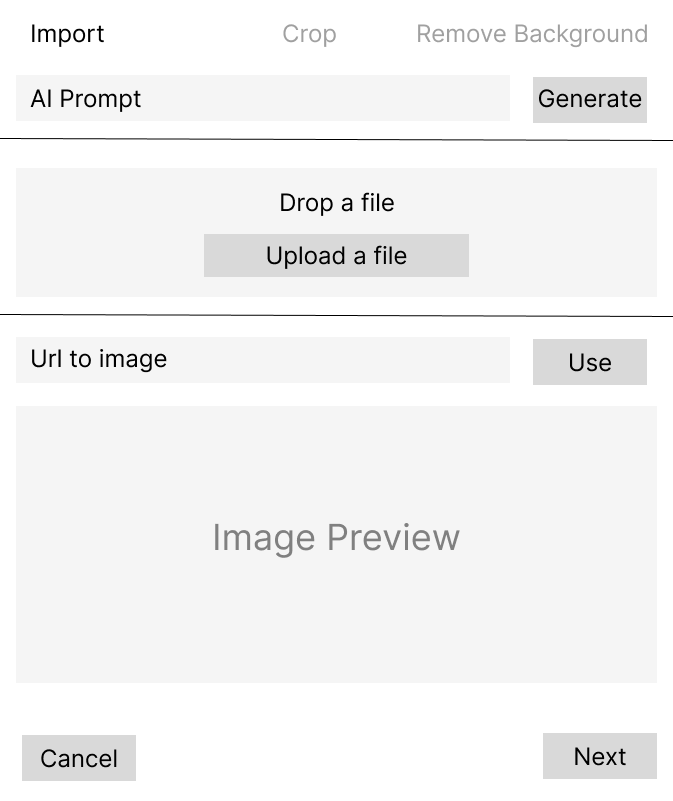
\includegraphics[width=\textwidth]{text/img/wireframes/Import image - import.png}}
        \caption{Step 2, import.}
        \label{fig:wireframes-import-import}
    \end{subfigure}
    \hspace{1cm}
    \begin{subfigure}{0.45\textwidth}
        \centering
        \fbox{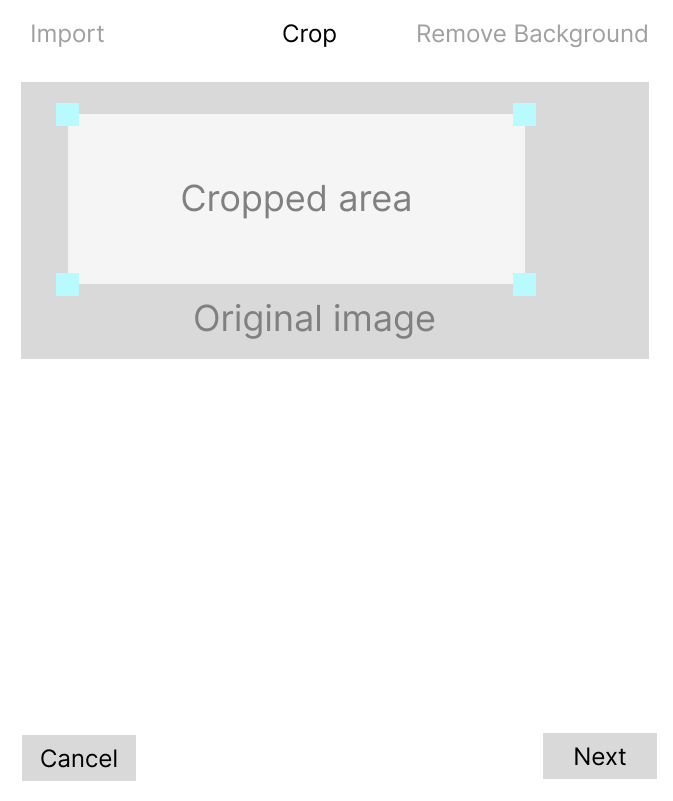
\includegraphics[width=\textwidth]{text/img/wireframes/Import image crop.png}}
        \caption{Step 2, crop.}
        \label{fig:wireframes-import-crop}
    \end{subfigure}
    \begin{subfigure}{0.45\textwidth}
        \centering
        \fbox{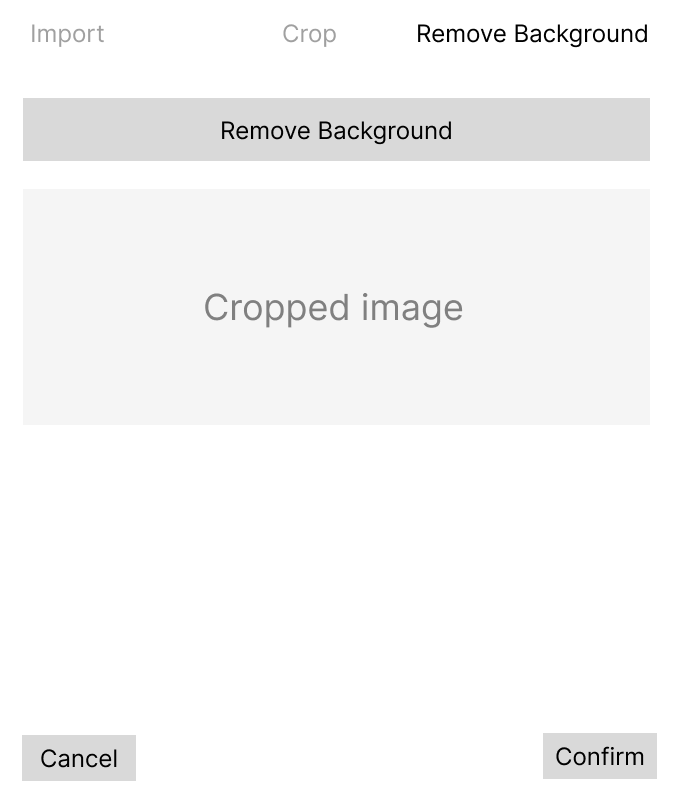
\includegraphics[width=\textwidth]{text/img/wireframes/Import image remove background.png}}
        \caption{Step 3, remove background, before \texttt{Remove Background} button is clicked.}
        \label{fig:wireframes-import-remove-background-before}
    \end{subfigure}
    \hspace{1cm}
    \begin{subfigure}{0.45\textwidth}
        \centering
        \fbox{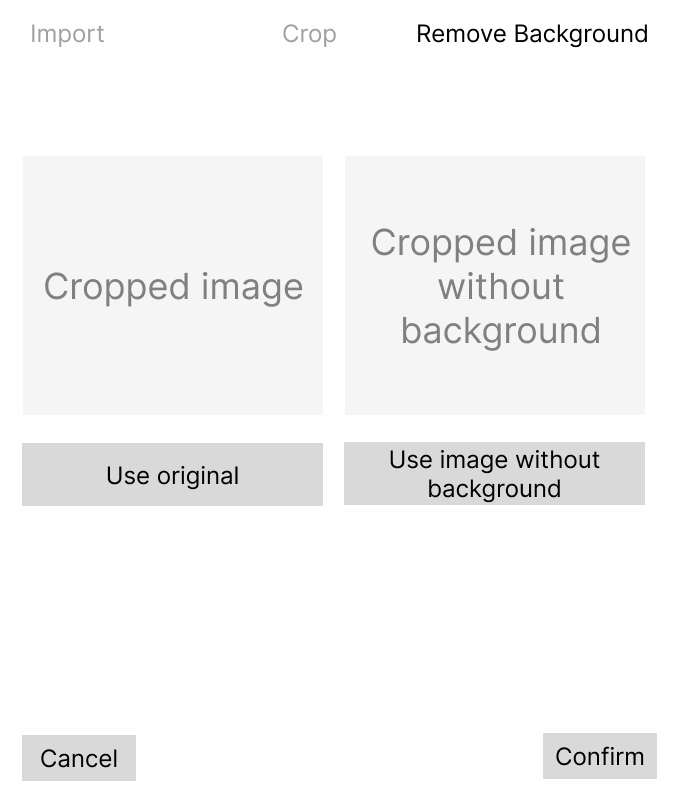
\includegraphics[width=\textwidth]{text/img/wireframes/Import image after removed.png}}
        \caption{Step 3, remove background, after \texttt{Remove Background} button is clicked.}
        \label{fig:wireframes-import-remove-background-after}
    \end{subfigure}
    \caption{Wireframes of the import image dialog.}
    \label{fig:wireframes-import-dialog}
\end{figure}

%%%%%%%%%%%%%%%%%%%%%%%%%%%%%%%%%%%%%%%%%%%%%%%
\section{Database Schema}
%%%%%%%%%%%%%%%%%%%%%%%%%%%%%%%%%%%%%%%%%%%%%%%

\label{sec:db-schema}

The database schema is shown in the figure \ref{fig:database}. The schema is designed to be as simple as possible, while still being able to support all the features of the application. The schema is designed to be easily extensible, so that new features can be added without having to change the schema.

The \texttt{Image} model acts as a foundational entity, encapsulating the core attributes of an image file within the system. The database itself doesn't store the image data directly, but rather a reference to the image file stored in the image storage. This allows for efficient storage and retrieval of images, as well as the ability to scale the image storage independently of the database.

The \texttt{TemplateText} and \texttt{TemplateImage} models define the components of a meme template, allowing dynamic placement and styling of text and images. They include attributes for positioning (\texttt{x}, \texttt{y}), dimension (\texttt{width}, \texttt{height}), styling (\texttt{fontSize}, \texttt{color}, \texttt{strokeColor}), and other visual properties (\texttt{scale}, \texttt{rotation}, \texttt{zIndex}). These models are crucial for creating templates that can be customized and reused, with \texttt{TemplateText} managing the textual elements and \texttt{TemplateImage} managing the imagery within templates.

The \texttt{Template} model serves as an aggregator, linking multiple \texttt{TemplateText} and \texttt{TemplateImage} objects to form a complete meme template. It includes a unique identifier, a name for the template, a visibility flag (\texttt{isPublic}), and relationships to the \texttt{Image} and \texttt{User} models, indicating the creator and the background image of the template.

The \texttt{Meme} model represents the final product, a personalized meme created by a user. It is linked to the User and Image models, connecting a meme to its creator and the image it utilizes.

The \texttt{Account} model is designed to manage user accounts, including authentication and authorization information. It supports integration with external authentication providers and maintains access and refresh tokens for user sessions. The unique constraint on the combination of \texttt{provider} and \texttt{providerAccountId} ensures that each external account is uniquely linked to a user account within the system.

The \texttt{Session} model handles user sessions, with a unique session token and an expiration date. This model is essential for tracking active user sessions and managing session expiration.

The \texttt{User} model represents individuals interacting with the system. It includes personal information such as name and email, with the email field being unique to prevent duplicate accounts. The User model has one-to-many relationships with \texttt{Account}, \texttt{Session}, \texttt{Template}, and \texttt{Meme}, indicating the various entities a user can have ownership of or association with.

Finally, the \texttt{VerificationToken} model is employed for account verification process when using email authentication. It includes a unique token and an expiration date, ensuring the token is used within a certain timeframe.

Each model is designed with a focus on modularity and extensibility, allowing for scalability as the system grows in complexity and user base. The relationships between models, particularly the one-to-many and many-to-one relationships, are carefully crafted to reflect the real-world interactions between the different entities. For instance, a User can create many Templates and Memes, but each Template or Meme is associated with exactly one User.

\begin{figure}
    \centering
    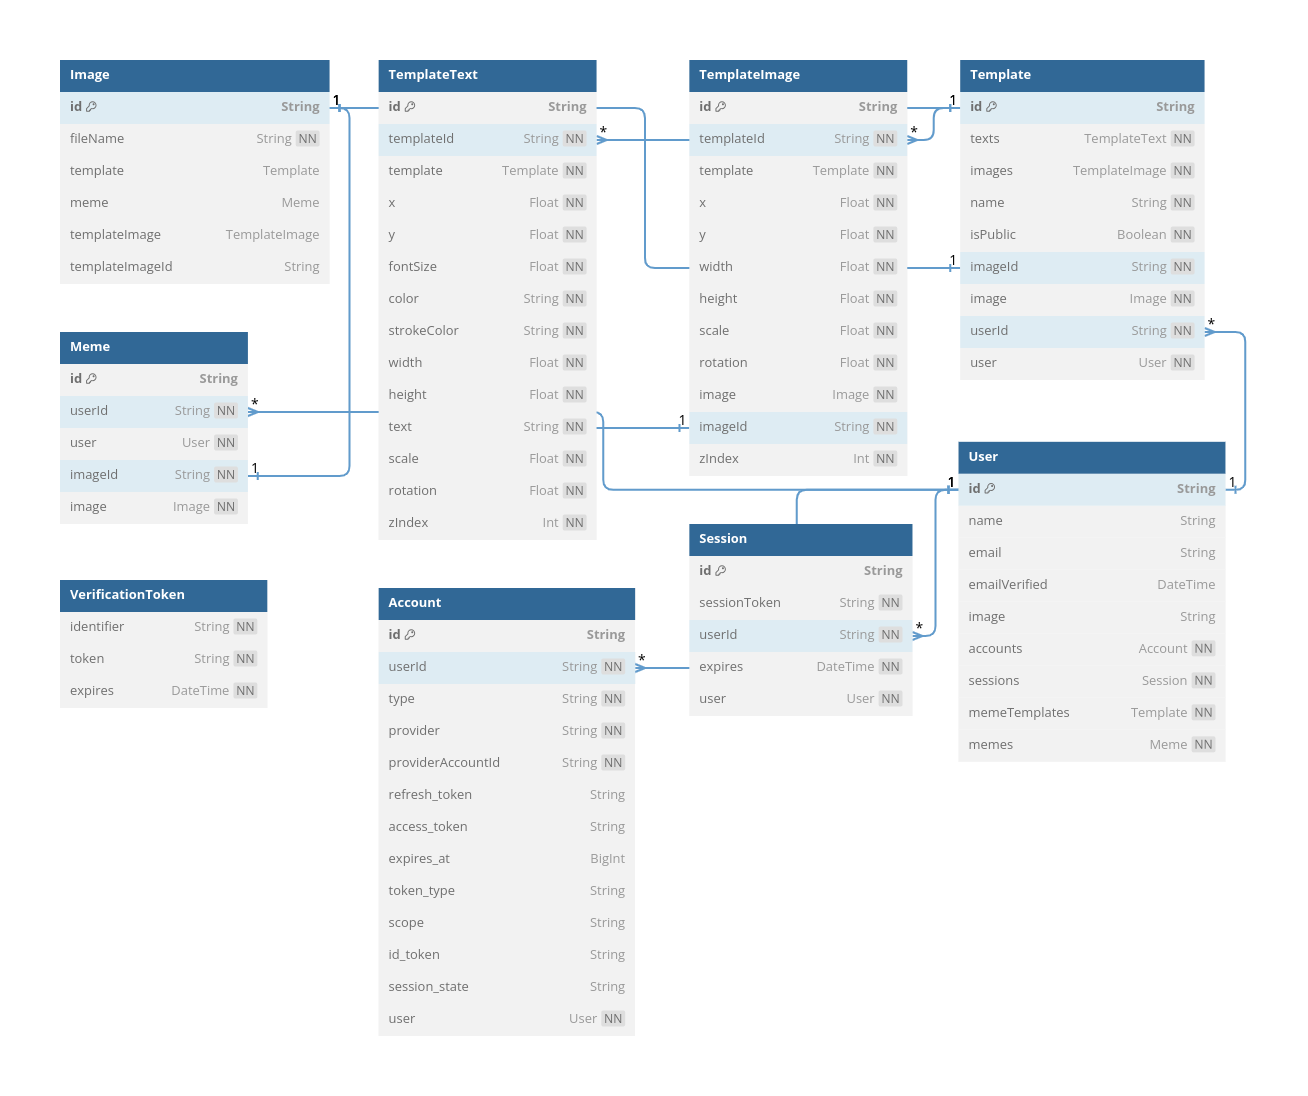
\includegraphics[width=\textwidth]{text/diagram/database-schema.png}
    \caption{Database schema.}
    \label{fig:database}
\end{figure}

%%%%%%%%%%%%%%%%%%%%%%%%%%%%%%%%%%%%%%%%%%%%%%%
\section{High-level architecture}
%%%%%%%%%%%%%%%%%%%%%%%%%%%%%%%%%%%%%%%%%%%%%%%

\begin{figure}
    \centering
    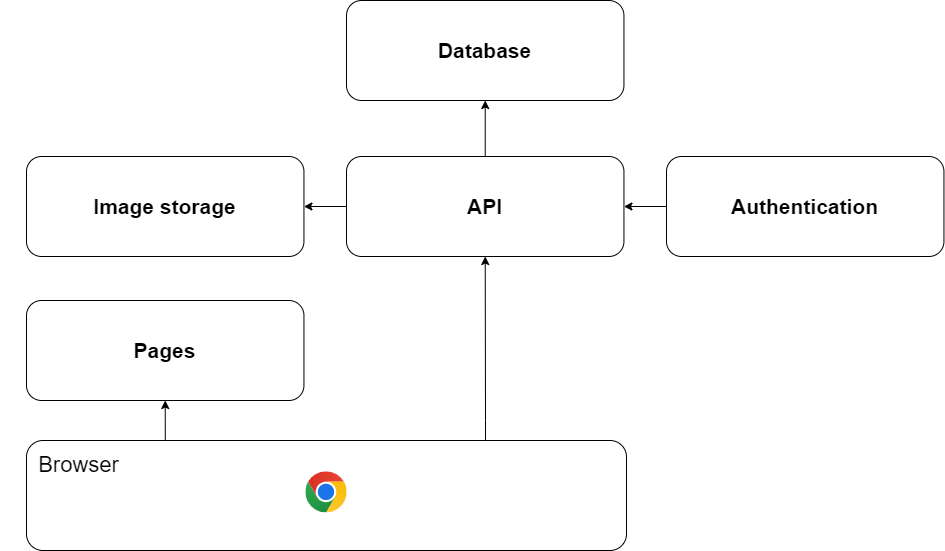
\includegraphics[width=\textwidth]{text/img/high-level.png}
    \caption{High-level architecture overview.}
    \label{fig:high-level}
\end{figure}

The architecture of the application is modular, consisting of five distinct but intercommunicating components.

\subsection{Pages}

The \texttt{Pages} module is primarily responsible for delivering the statically generated and server side generated frontend to the user's browser. This segment of the application encompasses all the static elements, as well as the necessary scripting to enable dynamic capabilities. The frontend interacts with the \acrshort{api} to facilitate access to an array of resources such as the database, image repository, and authentication mechanisms.

\subsection{API}

The \acrshort{api} mediates all interactions between the client-side browser and the other constituent components. It offers a suite of procedures that the frontend can invoke, thereby enabling the retrieval and submission of information as per user requests.

\subsection{Database}

The \texttt{Database} is a cornerstone component that holds all data related to the application, barring images. Its design ensures efficient storage, retrieval, and management of data, thereby supporting the application's operational integrity.

\subsection{Image Storage}

Dedicated to image management, the \texttt{Image Storage} component is tasked with housing all visual assets utilized by the application. This includes a variety of images such as meme content and images relating to templates, essential for the application's visual functionalities.

\subsection{Authentication}

The Authentication module is critical for maintaining the application's security. It interfaces with various authentication providers and manages email-based authentication processes. Additionally, it leverages the database for storing essential information related to user identities, accounts, and session data, thereby ensuring a secure and personalized user experience.

%---------------------------------------------------------------
\chapter{Development}
%---------------------------------------------------------------

This chapter describes the developmental framework of the application, providing a comprehensive overview of the various libraries implemented and the rationale behind their selection. It explains the synergistic integration of the application's components, detailing how each part contributes to the cohesive functioning of the whole system.

\section{Technologies}

This section has provided an overview of the framework selection process and the integration of various complementary technologies for the development of the application.

\subsection{Framework}

The initial step in determining the appropriate framework\cite{choose-tech-stack} for the application involved an analysis of the project requirements. This analysis encompassed understanding the application's functionality, and user experience goals and is described in detail in the previous chapter. Other requirements included my expertise, documentation, community support, and maturity of the framework.

The following frameworks were considered based on their popularity, measured by Stack Overflow Survey\cite{stack-overflow}, and relevance to the application's domain:

\begin{enumerate}
    \item Next.js
    \item Nuxt.js
    \item Remix
\end{enumerate}

Based on all factors mentioned above and internet research\cite{why-next}, mainly my extensive experience, Next.js was chosen as the framework for the application. Next.js is a React framework that provides a variety of features that are essential for the application, such as server-side rendering, static site generation, and routing. It also provides a variety of other features that are not essential for the application, but are useful, such as image optimization, internationalization, and many others.\cite{nextjs}

\subsubsection{Authentication}

\texttt{NextAuth} was selected as the authentication solution for its seamless integration with Next.js, the primary framework used for the application. It offers a straightforward and secure approach to handling user authentication and session management.\cite{why-next-auth} The simplicity of setting up providers for OAuth, Email, and other authentication mechanisms with \texttt{NextAuth} significantly accelerated the development process, while ensuring robust security and compliance with industry standards.

\subsubsection{State Management}

For state management within the application, \texttt{Zustand} was chosen for its minimalistic and straightforward API. Its non-boilerplate approach and ease of integration with React components made it an ideal choice for managing the application's state.\cite{why-zustand} Zustand's simplicity and efficiency in handling state across components helped in maintaining a clean and manageable codebase, improving both development speed and application performance.

\subsubsection{API Library}

\texttt{TRPC} was implemented to enable end-to-end type-safe API calls, enhancing the robustness and reliability of the application. It provided a simplified way of creating APIs without the need to define types and validation schemas multiple times, thereby reducing redundancy and potential for errors. This integration of \texttt{tRPC} brought a significant improvement in development efficiency and contributed to a more maintainable and error-resistant codebase.

\subsubsection{Database Management}

\texttt{Prisma} was incorporated as the database management tool, owing to its powerful and type-safe ORM capabilities. It offered an intuitive and straightforward way to interact with the database, ensuring a strong alignment with the application's data modeling and business logic requirements.\cite{why-prisma} Prisma's emphasis on type safety and its ease of use in defining and evolving the database schema played a pivotal role in enhancing the application's data integrity and overall backend efficiency.


\subsubsection{Database Backend}

SQLite was chosen as the database backend for its distinctive advantages that perfectly align with the needs of the project. A primary benefit of SQLite is its embedded nature within the application, eliminating the need for managing a separate database service. This integration simplifies the overall setup, which is crucial for developer velocity.

Starting up a new database with SQLite is remarkably uncomplicated compared to other databases like Postgres. There's no intricate setup process; it's essentially just a file. This simplicity extends to production migrations and seed operations, which can be executed with minimal effort. The application heavily utilizes these features, with the database being created and seeded during the build process. This approach ensures that the application is ready to use immediately after deployment, with no additional setup required.

Furthermore, this ease of use significantly benefits the testing phase of development. Complex database setups often lead to time-consuming evaluations of how to mock databases at the ORM level to avoid the challenges of running and connecting to a database during testing. SQLite, being just a file, simplifies this process substantially. Each test can have its own isolated database environment with minimal setup, allowing for more efficient and accurate testing scenarios. This level of ease and efficiency in setting up isolated test environments is harder to achieve with other database systems.\cite{why-sqlite}

%%%%%%%%%%%%%%%%%%%%%%%%%%%%%%%%%%%%%%%%%%%%%%%
\section{Application design}
%%%%%%%%%%%%%%%%%%%%%%%%%%%%%%%%%%%%%%%%%%%%%%%

\begin{figure}
    \centering
    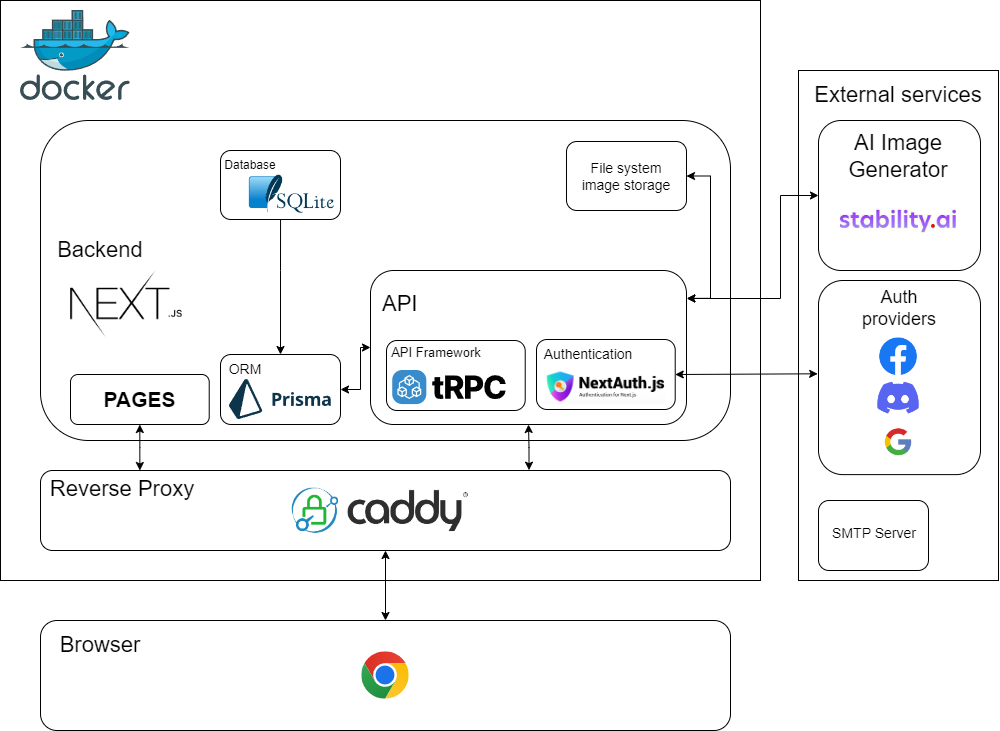
\includegraphics[width=\textwidth]{text/img/low-level.png}
    \caption{Application diagram.}
    \label{fig:low-level}
\end{figure}

\newacronym{https}{HTTPS}{Hypertext Transfer Protocol Secure}
\newacronym{http}{HTTP}{Hypertext Transfer Protocol}
\newacronym{smtp}{SMTP}{Simple Mail Transfer Protocol}
\newacronym{ai}{AI}{Artificial Intelligence}

Figure \ref{fig:low-level} presents the high-level architecture of the application, showcasing the interaction between its components as detailed in the preceding section. The system utilizes Docker for containerization, streamlining deployment, which is further elaborated in Section \ref{sec:deployment}.

At its core, the application consists of statically generated pages and an \acrshort{api} for client-server interaction. Statically generated pages enhance performance by reducing server load, while the \acrshort{api} ensures efficient data transfer and processing. Prisma, serving as the \acrfull{orm}, abstracts database interactions, simplifying database operations.\cite{prisma}

Authentication is streamlined via three external providers, optimizing the sign-in and registration workflows. There is also an email option, which utilizes an external \acrfull{smtp} server.

The application offers its users the ability to generate images using text-to-image \acrfull{ai} models. This functionality is facilitated by an external \acrshort{api} that is integrated into the application.

%%%%%%%%%%%%%%%%%%%%%%%%%%%%%%%%%%%%%%%%%%%%%%%
\section{Configuration}
%%%%%%%%%%%%%%%%%%%%%%%%%%%%%%%%%%%%%%%%%%%%%%%

The application is configurable through the use of environment variables. The variables can either be set as environment variables on the host system, or they can be filled into the .env file in the directory from which the application is launched. The environment variables are validated on startup, and the application will not start if any of the required variables are missing. The environment variable schema is configured in the \texttt{src/env.mjs} file.

This section describes all the configuration options and the environment variables that are used to configure them.

\subsection{Data Storage}

The database configuration within the application is specified by the \texttt{DATABASE\_URL} environment variable, which is a standard practice for defining connection strings. In the context of this application's architecture, the flexibility to switch between different database providers is restricted by the limitations of the Prisma framework.\cite{prisma-sqlite} As such, SQLite is the exclusive database provider utilized. The format of the \acrshort{url} for connecting to the SQLite database is explicitly structured as \texttt{file:file-location}, which indicates the file path where the SQLite database is located on the filesystem. By using this approach, the application benefits from SQLite's simplicity and ease of use, while also allowing for the database to be easily referenced and managed within the application's codebase.

The configuration for image storage within the application is governed by the \texttt{IMAGE\_UPLOAD\_DIR} environment variable. This variable is responsible for specifying the directory path where all images are to be stored. It is crucial to ensure that the designated directory is already established on the server's filesystem and that the necessary permissions are set so that the application has the requisite write access. The proper configuration of this environment variable is essential for the seamless operation of the image upload and storage features of the application.

\subsection{Authentication}
\label{sec:authentication}

\texttt{NextAuth}, a critical component for handling authentication in the application, necessitates the configuration of essential environment variables as outlined in its documentation\cite{auth-options}. The \texttt{NEXTAUTH\_URL} variable is pivotal, required to be set to the canonical \acrshort{url} of the deployed website, ensuring that OAuth callbacks are correctly resolved. Furthermore, for the sake of security, the \texttt{NEXTAUTH\_SECRET} is used as an encryption key for session tokens and for hashing email verification tokens, enhancing the integrity and confidentiality of the authentication process.

In an effort to facilitate a flexible and dynamic authentication system, the default \texttt{NextAuth} configuration has been augmented. This customization permits the activation of different authentication providers through environment variable configurations, adhering to the principle of infrastructure as code. Presently, the system supports up to three distinct OAuth providers and also an email sign in capability.

The built-in OAuth providers supported by \texttt{NextAuth} are extensive\cite{auth-oauth}, and this application harnesses the capability to integrate three popular services: Facebook, Google, and Discord. Each service requires the setting of two specific environment variables: \texttt{[PROVIDER]\_CLIENT\_ID} and \texttt{[PROVIDER]\_CLIENT\_SECRET}. These variables function as the application's credentials for interacting with the respective OAuth service, and their values are crucial for the initiation and secure maintenance of OAuth flows. The process of setting up each provider is detailed in the \texttt{NextAuth} documentation\cite{auth-oauth}. The application will enable any of these providers if both of their respective environment variables are set.

The configuration of the email provider is determined by two essential environment variables. The \texttt{EMAIL\_SERVER} variable is designated to define the SMTP server details that \texttt{NextAuth} will utilize to send out the authentication emails. The expected format for the \texttt{EMAIL\_SERVER} variable aligns with the specifications provided in the \texttt{Nodemailer} library's documentation\cite{nodemailer-smtp}, ensuring compatibility and ease of setup.

Additionally, the \texttt{EMAIL\_FROM} variable defines the sender's email address for all outgoing messages. This address represents the application in the users' inboxes and should be chosen to reflect the application's identity and to avoid being filtered as spam. Email sign in is enabled if both of these variables are set.

\subsection{AI Image Generation}

The application utilizes an external \acrshort{api} for generating images from text. The \acrshort{api} is provided by the \texttt{stability.ai platform}.\footnote{https://platform.stability.ai} The \texttt{stability.ai platform} is a paid service, and it requires a registered account to be able to take advantege of its \acrshort{api}. The \texttt{STABILITY\_AI\_API\_KEY} environment variable is used to specify the \acrshort{api} key, which is used to authenticate the application with the \texttt{stability.ai platform}.

%%%%%%%%%%%%%%%%%%%%%%%%%%%%%%%%%%%%%%%%%%%%%%%
\section{API}
%%%%%%%%%%%%%%%%%%%%%%%%%%%%%%%%%%%%%%%%%%%%%%%
\newacronym{json}{JSON}{JavaScript Object Notation}

This section dives deeper into the implementation of all the application \acrshort{api} endpoints and procedures. Most of the \acrshort{api} functionalities are implemented using the \texttt{tRPC} library, except for the endpoints which send images between the frontend and backend. TRPC only supports sending payloads which are serializable to \acrfull{json}\cite{trpc-files} which is a limitation that makes \texttt{tRPC} not a suitable tool for this purpose. Images could be serailzed using \texttt{base64} encoding, but that is generally considered to be a bad practice because of the performance and size limitations\cite{base64}.

\subsection{Image upload}
\label{sec:api-image-upload}

\newacronym{uuid}{UUID}{Universally Unique Identifier}

This endpoint handles \texttt{POST} operations to the \texttt{/api/image-upload} route, processes the file upload using \texttt{multer}, and responds with the path of the uploaded image. The \acrshort{api} endpoint configures Next.js to handle multipart/form-data requests, which are essential for file uploads, by disabling the default JSON body parsing. This is a crucial aspect because image uploads involve binary data that doesn't fit into the standard JSON format. By customizing the \texttt{bodyParser} configuration, the API ensures that the raw data from multipart forms can be processed correctly, catering specifically to the needs of file upload operations.

A notable feature of this API is the implementation of a unique filename generation mechanism for each uploaded image. This is achieved using the \texttt{uuid} library to generate an \acrfull{uuid} for each file, ensuring that each uploaded image has a distinct filename, thereby eliminating conflicts and overwrites in the server's storage. Additionally, the API leverages the \texttt{mime-types} library to accurately determine and append the appropriate file extension based on the MIME type of the uploaded file. This approach contributes to better organization and retrieval of uploaded files.

The API employs \texttt{multer}, a popular middleware for handling \texttt{multipart/form-data} \acrshort{http} requests, to manage the incoming file data. The configuration of \texttt{multer} is tailored to store files in a designated directory defined by the configuration environment variables, with filenames determined by the aforementioned unique naming strategy. The final part of the API is an express route set up using \texttt{next-connect} - a minimalist framework for routing and middleware.

\subsection{Generate AI Image}

This endpoint handles \texttt{POST} operations to the \texttt{/api/generate-ai-image} route and facilitates the interaction with an external AI image generation service, specifically Stability AI's platform. The function is structured to respond to HTTP requests by generating images based on text prompts provided by the user, showcasing integration with an advanced AI-powered service in a web application.

The handler function first checks for the presence of a 'prompt' in the query parameters of the request. If the prompt is missing, it responds with a 400 status code  and an error message, ensuring that the necessary input for generating an image is provided. This is a crucial step to validate the incoming request and maintain the integrity of the API's functionality.

Once a valid prompt is received, the handler makes a \texttt{POST} request to the Stability AI's API endpoint. It constructs the request with appropriate headers, including the necessary API key obtained from the environment variables. The body of the request includes the text prompt, along with specifications for the generated image such as its height, width, number of samples, and steps for the generation process. These parameters are essential for tailoring the image generation to the specific requirements of the application.

The response from the Stability AI API is expected to contain the generated artifacts in the form of a base64-encoded string representing the generated image. The handler function checks whether it received the artifacts and forwards them to the client. However, if the call to the \acrshort{api} didn't succeed, a 500 status code with an appropriate error message is returned.

\subsection{Remove background}

This endpoint handles \texttt{POST} operations to the \texttt{/api/remove-background} route and facilitates the interaction. It employs the same techniques for image upload and manipulation as the \texttt{image-upload} endpoint described in Section \ref{sec:api-image-upload} with some key differences. The \texttt{multer} configuration for this endpoint does not specify an upload directory, but stores the received images into memory instead.

The handler utilizes the \texttt{sharp} and \texttt{rembg} libraries to process the uploaded image and remove its background. First, the handler has to check whether an image file has been uploaded. If no file is found, a 400 status response is sent with a relevant message. Otherwise, the code processes the uploaded image using \texttt{sharp} and \texttt{rembg}, removing the background. If successful, the processed image data is returned as a response with a 200 status. In the case of errors during image processing, a 500 status is returned with error details.

\subsection{tRPC}

TRPC has been instrumental in optimizing interactions between the frontend and the database. By facilitating direct, procedure-based communication between the client and server, it eliminates the complexities and overheads associated with traditional REST or GraphQL APIs. This streamlined approach, enhanced by TypeScript's strong typing, ensures consistent data structures across both ends, significantly reducing runtime errors and improving data integrity, especially in complex database operations. The integration of TRPC thus not only accelerates development cycles but also fortifies the application's reliability.\cite{trpc} The section is structured into router subsections, each of which describes the procedures implemented within the router.

\subsubsection{Profile Router}

The profile router encapsulates all the procedures related to user profile management. It contains two primary mutations: \texttt{updateUserName} and \texttt{updateProfileImage}. Both mutations are secured with \texttt{protectedProcedure}, indicating that they require user authentication. Each mutation accepts a single string input; username and profile image \acrshort{url}. The core functionality involves updating the user's name or profile image in the database using \texttt{Prisma}, with the current user's ID obtained from the session context supplied by \texttt{NextAuth}.

\subsection{Template Router}

The template router handles all the interactions related to meme templates. Its procedures are secured with \texttt{protectedProcedure}, ensuring that only authenticated users can access them

\noindent
\begin{longtable}{@{}>{\raggedright\arraybackslash}p{3cm} p{11cm}}
    \hline
    \multicolumn{2}{c}{\textbf{createTemplate}}
    \\
    \hline
    \textbf{Description}  & This procedure enables authenticated users to create new templates.
    \\
    \textbf{Parameters}   & Input object with properties: 'name' (string), 'isPublic' (boolean), 'fileName' (string), 'texts' (array of objects validated by the database schema), 'images' (array of objects validated by the database schema).
    \\
    \textbf{Operations}   & Authenticates the user, creates a new image and template in the database, and adds associated texts and images. Each text and image is validated and processed individually, ensuring data integrity and consistency.
    \\
    \textbf{Return value} & Returns an object including the newly created template details, along with the texts and images associated with it.
    \\
    \hline
    \multicolumn{2}{c}{\textbf{updateTemplate}}
    \\
    \hline
    \textbf{Description}  & This procedure is designed for updating existing templates.
    \\
    \textbf{Parameters}   & Input object with properties: 'template' (object with template details, excluding sensitive fields like 'imageId' and 'userId'), 'texts' (array of objects validated by the database), 'images' (array of objects validated by the database schema).
    \\
    \textbf{Operations}   & Performs ownership verification of the template, deletes existing texts and images related to the template, then updates the template with the new data.
    \\
    \textbf{Return value} & The response includes an updated template object, featuring the new sets of texts and images, indicative of a complete and secure update operation.
    \\
    \hline
    \multicolumn{2}{c}{\textbf{deleteTemplate}}
    \\
    \hline
    \textbf{Description}  & This procedure allows users to delete their templates.
    \\
    \textbf{Parameters}   & Input object with a single field 'id' (string), specifying the template to be deleted.
    \\
    \textbf{Operations}   & Checks if the user is authorized to delete the specified template. Upon successful verification, proceeds to delete the template from the database, ensuring data consistency and security.
    \\
    \textbf{Return value} & Doesn't return any value, but the procedure throws an error if something unexpected happens or if the user is not authorized to delete the template.
    \\
    \hline
    \multicolumn{2}{c}{\textbf{getTemplate}}
    \\
    \hline
    \textbf{Description}  & The procedure is a public procedure for retrieving specific templates.
    \\
    \textbf{Parameters}   & A single input 'id' (string) to identify the template to be fetched.
    \\
    \textbf{Operations}   & Includes conditional logic to ensure that private templates are accessible only by their owners. Retrieves a specific template from the database, along with its associated images and texts.
    \\
    \textbf{Return value} & The detailed representation of the template, including associated images and texts.
    \\
    \hline
    \multicolumn{2}{c}{\textbf{getInfiniteTemplates}}
    \\
    \hline
    \textbf{Description}  & This procedure is designed to fetch templates in a paginated manner.
    \\
    \textbf{Parameters}   & Input object with properties: 'fetch' (enum: fromUser, public, all), 'limit' (number, min: 1, max: 100), 'cursor' (string, nullish), 'searchString' (string, optional).
    \\
    \textbf{Operations}   & Conducts a paginated query based on the input parameters, retrieving templates from the database. The operation involves filtering templates, providing a mechanism for fetching data in a manageable and scalable way.
    \\
    \textbf{Return value} & An object containing the fetched items and a 'nextCursor' for pagination, enabling the frontend to fetch the next page of items.
    \\
\end{longtable}

\subsubsection{Meme Router}

\noindent
\begin{longtable}{@{}>{\raggedright\arraybackslash}p{3cm} p{11cm}}
    \hline
    \multicolumn{2}{c}{\textbf{createMeme}}
    \\
    \hline
    \textbf{Description}  & This procedure enables authenticated users to create new memes.
    \\
    \textbf{Parameters}   & Input object with property: 'fileName' (string).
    \\
    \textbf{Operations}   & Authenticates the user, creates an image entry in the database using the provided file name, then creates a meme associated with the image and the current user.
    \\
    \textbf{Return value} & Returns the newly created meme object, including the meme details and the path to the associated image.
    \\
    \hline
    \multicolumn{2}{c}{\textbf{deleteMeme}}
    \\
    \hline
    \textbf{Description}  & The procedure allows users to delete their memes.
    \\
    \textbf{Parameters}   & Input object with property: 'id' (string) specifying the meme to be deleted.
    \\
    \textbf{Operations}   & Verifies the ownership of the meme, then proceeds to delete both the meme and its associated image from the database.
    \\
    \textbf{Return value} & Doesn't return any value, but the procedure throws an error if something unexpected happens or if the user is not authorized to delete the template.
    \\
    \hline
    \multicolumn{2}{c}{\textbf{getInfiniteMemes}}
    \\
    \hline
    \textbf{Description}  & This procedure is designed for fetching memes using pagination to limit the number of memes returned in each query.
    \\
    \textbf{Parameters}   & Input object with properties: 'limit' (number, min: 1, max: 100), 'cursor' (string, nullish)
    \\
    \textbf{Operations}   & Retrieves memes created by the current user in a paginated manner, based on the provided limit and cursor for pagination.
    \\
    \textbf{Return value} & An object containing the fetched memes and a 'nextCursor' for pagination.
    \\
\end{longtable}

%%%%%%%%%%%%%%%%%%%%%%%%%%%%%%%%%%%%%%%%%%%%%%%
\section{State Management}
\label{sec:state}
%%%%%%%%%%%%%%%%%%%%%%%%%%%%%%%%%%%%%%%%%%%%%%%

State management is a critical aspect of building robust and maintainable React applications. It allows developers to handle data and application state in a predictable and efficient manner. State management solutions, like Zustand, simplify the process of managing state in React applications.\cite{zustand-setup} This section explains in details how Zustand is used and how its features are leveraged to efficiently manage application data.

The module contains a single store with all the application data and functions for manipulating the data. This store is shared across the while application and every page/component has access to its data and function The individual pieces that make up the store are outlined in this section. Each piece has a TypeScript type definition which illustrates the structure of the data and the functions.

\subsection{Popups}
\begin{verbatim}
export type PopupType = {
    id: number
    type: 'info' | 'warning' | 'success' | 'error'
    message: string
}

type PopupState = {
    popupCounter: number
    popups: PopupType[]
    addPopup: (popup: Omit<PopupType, 'id'>) => void
    removePopup: (id: number) => void
}
\end{verbatim}

This part of the state is used to display pop-up notifications. On the screen.

The \texttt{PopupType} interface defines the structure of pop-up notifications and ensures consistency in how pop-up notifications are defined and rendered.

The \texttt{PopupState} type defines the state for the store. It includes a \texttt{popupCounter} to keep track of the unique IDs for pop-ups, an array to store the pop-up notifications, an \texttt{addPopup} function to add new pop-ups to the state, and a \texttt{removePopup} function to remove pop-ups by their unique IDs.

The \texttt{addPopup} function takes a popup object as a parameter, omits the id field (which is automatically generated), and pushes the new pop-up into the popups array. Additionally, it sets a timeout to remove the pop-up after a specified duration defined by a constant \texttt{POPUP\_TIMEOUT}, ensuring that pop-ups disappear automatically. The unique ID assigned to each pop-up is essential to identify and remove them later.

The \texttt{removePopup} function is responsible for removing pop-ups by their unique ID.

\subsection{Dialogs}
\begin{verbatim}
type DialogType = 'addImage' | 'save' | 'exportMeme'

type DialogState = {
    dialogs: {
        [key in DialogType]: boolean
    }
    setDialog: (dialog: DialogType, open: boolean) => void
}
\end{verbatim}

This section of the state allows for easy control of different dialogs' open or closed states.

The \texttt{DialogState} type contains a \texttt{dialogs} object, where each key corresponds to a \texttt{DialogType}, and the associated value indicates whether the respective dialog is open or closed. This structure ensures that the state of each dialog can be tracked individually.

The \texttt{setDialog} function is designed to update the state of a specific dialog, effectively toggling the visibility of the specified dialog. It takes two parameters: \texttt{dialog} to specify which dialog to update and \texttt{open} to indicate whether to open or close the dialog.

\subsection{Import Image}
\begin{verbatim}
export type ImageImportStep = 'import' | 'crop' | 'remove-bg'

type ImageImportState = {
    isImportingBackground: boolean
    importCurrentStep: ImageImportStep
    importedImage: File | null
    importNextStep: (image: File) => void
    openImport: (isImportingBackground?: boolean) => void
}
\end{verbatim}

This part of the state is designed to facilitate the step-wise import and manipulation of images, which is used when importing a background of a template or an image as a part of a template. It defines the \texttt{ImageImportState} type, which encompasses essential attributes and functions. Firstly, it includes \texttt{isImportingBackground} to destinguish between an image being imported as a background or as a part of a template. The \texttt{importCurrentStep} attribute is used to keep track of the current import step defined by \texttt{ImageImportStep}, and \texttt{importedImage} to hold the imported image file.

The \texttt{importNextStep} function allows seamless transitions between import steps. Depending on the current step, it updates the state accordingly. For example, if the current step is \texttt{import}, it advances to \texttt{crop}, and if it's \texttt{crop}, it proceeds to \texttt{remove-bg}. When the last step is advanced from, the image is either set as the background or it is added to the template's images.

The \texttt{openImport} function initializes the image import process. It accepts an optional parameter \texttt{isImportingBackground} to determine the type of import, but can default to the value in the store. It resets the state and opens the import dialog, preparing the application for the user to begin importing and manipulating images.

\subsection{Template Texts}
\begin{verbatim}
type FTemplateText = Partial<TemplateText> &
    Omit<TemplateText, 'id' | 'templateId'>

type TextState = {
    texts: {
        [key: string]: FTemplateText
    }
    addText: () => void
    deleteText: (key: string) => void
    updateText: (key: string, text: FTemplateText) => void
}
\end{verbatim}
This chunk of the state manages text elements within a meme template, enabling dynamic addition, modification, and deletion of text elements. It defines the \texttt{TemplateTextState} type, which includes attributes and functions for handling text elements within a meme template.

The \texttt{texts} property stores text elements where each key represents a unique identifier for each element, and the associated value is an object containing various properties of the text which are defined by the database schema. It initially starts as an empty object, but text elements are added dynamically.

The \texttt{addText} function is responsible for adding a new text element to the texts object. It generates a unique identifier using the \texttt{uuid} library and initializes the properties of the text element with default values, such as position at (0,0), default colors, width and height, an empty text string, and other styling properties. The zIndex property is incremented to ensure that the next element appears on top of existing ones.

The \texttt{updateText} function allows for updating the properties of a specific text element identified by its \texttt{id}. It receives the \texttt{id} and the new text properties and updates the state by replacing the existing text element properties with the new ones.

\texttt{deleteText} function removes a text element from the state based on its \texttt{id}. It uses the delete operator provided by javascript to delete the corresponding text element from the texts object, effectively removing it from the template.

\subsection{Template Images}
\begin{verbatim}
 type FTemplateImage = Omit<TemplateImage, 'id' | 'templateId' | 'imageId'> &
    Partial<Pick<TemplateImage, 'id' | 'templateId' | 'imageId'>> &
    (
        | { imageFile: File; imageUrl?: never }
        | { imageUrl: string; imageFile?: never }
    )

type ImageState = {
    images: {
        [key: string]: FTemplateImage
    }
    addImage: () => void
    updateImage: (key: string, image: FTemplateImage) => void
    deleteImage: (key: string) => void
}
\end{verbatim}

This part of the state enables dynamic addition, modification, and deletion of image elements in templates. It also integrates with the \texttt{openImport} function to simplify the process of adding images by triggering the image import dialog, which handles all to logic realted to importing images. The underlying images are either represented by binaray data in the form of a \texttt{File} object or by a link to an image, depending on whether they have been uploded to the server or not.

The \texttt{addImage} function is responsible for adding a new image element to the images object. When called, it invokes the \texttt{openImport} function, which initiates the image import process.

The \texttt{updateImage} function allows for updating the properties of a specific image element identified by its \texttt{id}. It receives the \texttt{id} and the new image properties, and it updates the state by replacing the existing image element properties with the new ones. This function is essential for customizing the images within the template, like editing its size, rotation and other properties.

The \texttt{deleteImage} function removes an image element from the state based on its \texttt{id}. It uses the javascript delete operator to delete the corresponding image element from the images object, effectively removing it from the template.

\subsection{Template}
\begin{verbatim}
type TemplateState = {
    template: Pick<Template, 'isPublic' | 'name'> & Partial<Template>
    currentZIndex: number
    switchZIndexes: (
        obj1: { type: 'text' | 'image'; id: string },
        obj2: { type: 'text' | 'image'; id: string }
    ) => void
    updateTemplate: (updates: Partial<Template>) => void
    saveTemplate: (overwrite: boolean) => void
    useTemplate: (id: string) => Promise<void>
}
\end{verbatim}

This part of the state is responsible for managing the currently edited template. It defines the \texttt{TemplateState} type, which includes the \texttt{template} object, which stores the template details, and the \texttt{currentZIndex} attribute, which is used to keep track of the current highest z-index value.

The \texttt{switchZIndexes} function is used to switch the z-indexes for text and image elements in the template. It takes two elements as parameters, each containing the type of the element and its \texttt{id}. It finds the objects in the template and switches their z-indexes, ensuring that they appear in the correct order when rendered.

The \texttt{updateTemplate} function allows for updating the template information by merging the provided updates into the existing template state, ensuring that the template data remains up-to-date. When updating the template, the images that were previously uploaded are not uploaded, the link to the image is reused.

The \texttt{useTemplate} retrieves a template from an \acrshort{api}, initializes the application's state with the template data, and sets the background, texts, and images. It also handles z-index calculations to ensure proper layering of elements.

The \texttt{saveTemplate} function is responsible for saving meme templates. It checks whether the template is being updated or created and makes the appropriate API calls to save the template and associated elements (images and texts). Images have to firstly be uploaded using the \texttt{upload-image} \acrshort{api} endpoint before the links can be sent using \texttt{tRPC} to the database. The function also handles the validation of required data and displays success or error messages using pop-up notifications.

\subsection{Meme}

\begin{verbatim}
type MemeState = {
    exportedMeme: null | string
    setExportedMeme: (exportedMeme: null | string) => void
    exportMeme: (meme: Blob, authenticated?: boolean) => void
}
\end{verbatim}

This portion of the state is responsible for handling the export of meme images. It takes care of both authenticated and non-authenticated scenarios, ensuring that the exported meme image is appropriately stored in the \texttt{exportedMeme} state and saved in the database and image storage through the usage of \texttt{image-upload} \acrshort{api}. Additionally, it provides error handling and user feedback through pop-up messages in case of any issues during the export process.

The \texttt{setExportedMeme} function is responsible for setting the \texttt{exportedMeme} variable to a provided value.

The \texttt{exportMeme} function initiates the process of exporting a meme image. It takes two parameters: \texttt{memeFile} (the meme image file) and \texttt{authenticated} (a boolean flag indicating whether the user is authenticated). The function begins by checking the application's current state.

If the background image is missing, it triggers a pop-up error message indicating that a meme cannot be created without a background.

If the user is authenticated, the function proceeds to upload the meme image file using the \texttt{upload-image} \acrshort{api} endpoint. Upon successful upload, it makes an API call to create a meme with the uploaded image file and obtains the meme's image path. The \texttt{exportedMeme} state is then set to the meme's image path.

If the user is not authenticated, the image is not uploaded to the server. The \texttt{exportedMeme} state to a \acrshort{url} created from the provided \texttt{memeFile}. This URL can be used to display the meme image to the user without persisting it into the database.


% \subsection{Upload Image Helper}
% % \label{sec:upload-image-helper}

% The \texttt{uploadImageHelper} function is a function, that takes an image as a parameter and uploads that image using the image upload API defined in \autoref{sec:api-image-upload}. It creates a new \texttt{FormData} object, which can be used to construct a set of key/values pairs representing a form \cite{form-data}. The image is added to this set and then the \texttt{FormData} object is passed to the fetch function, which calls the image upload API endpoint. The result is parsed into JSON and checked, whether it contains the path property, which would be the path to the uploaded image. This path is returned, otherwise, an error occurs.

\subsection{Persisting state}

To ensure that the user's progress with edited templates is persisted and retained even after a page refresh, the application leverages the \texttt{persist} middleware provided by Zustand. This middleware offers various options for storing and serializing state. In this case, the application serializes the state into \acrshort{json} format and saves it to session storage. However, some properties are intentionally excluded from persistence as they are either unable to be serialized into \acrshort{json}, like images, or they aren't needed on refresh, like popups.


%%%%%%%%%%%%%%%%%%%%%%%%%%%%%%%%%%%%%%%%%%%%%%%
\section{Styles}
%%%%%%%%%%%%%%%%%%%%%%%%%%%%%%%%%%%%%%%%%%%%%%%
\newacronym{css}{CSS}{Cascading Style Sheet}
\newacronym{html}{HTML}{Hyper Text Markup Language}

In the realm of web applications, the integration of \acrfull{css} is imperative for transforming a plain text-on-white background interface into a visually appealing and distinctive user experience.\cite{what-is-css} Over time, various approaches have emerged for crafting styled components using \acrshort{css}. One particularly promising method is exemplified by the Tailwind CSS library.\cite{why-tailwind}

Tailwind \acrshort{css}, introduces a paradigm centered around utility classes. This approach offers immense convenience to developers. Instead of manually crafting extensive \acrshort{css} files, developers can directly apply utility classes within their \acrshort{html} markup. This streamlined workflow empowers developers to swiftly implement styles and layouts, enhancing development efficiency.

Moreover, the application under consideration leverages the DaisyUI library. DaisyUI aligns closely with Tailwind \acrshort{css} but extends its capabilities by bundling additional functionalities. This synergy equips developers with an extensive toolkit for designing and styling components, reinforcing the application's visual appeal and usability.\cite{why-daisy}

In essence, the combination of Tailwind \acrshort{css} and DaisyUI within this application signifies a modern and efficient approach to web styling. It exemplifies the benefits of utility classes and the convenience of accessible styled components, ultimately contributing to a polished and user-friendly interface.

%%%%%%%%%%%%%%%%%%%%%%%%%%%%%%%%%%%%%%%%%%%%%%%
\section{Components}
%%%%%%%%%%%%%%%%%%%%%%%%%%%%%%%%%%%%%%%%%%%%%%%

This section describes all the notable components that are used throughout the application. Certain components play a central role in the entire application and are therefore organized within the dedicated \texttt{common} folder. These components are used on multiple pages and are therefore not tied to a specific page.

There is also a dedicated \texttt{layout} folder, which contains components that are used to define the layout of the application. These components are used on every page and are therefore not tied to a specific page.

The rest of the components are organized into folders based on the page they are used on.

\subsection{Alert}
\newacronym{svg}{SVG}{Scalable Vector Graphics}

The \texttt{Alert} component offers a convenient way to display informative messages to users while maintaining a consistent and visually appealing user interface. It can be easily integrated into various parts of the application where notifications or alerts are required, enhancing the user experience by providing clear and context-specific feedback.

These alerts can convey different messages, such as informational, warning, success, or error messages, to the user. The component is designed to be versatile, allowing developers to customize the type of alert and the content displayed within it.

The type of the displayed alert message is customizable by providing a \texttt{type} property. This property determines the visual style and icon associated with the alert, making it easier to convey the nature of the message to the user. The available types include 'info,' 'warning,' 'success,' and 'error.'

Internally, the component utilizes \acrfull{svg} icons to represent the different alert types, which are fetched from the icons object based on the specified type. These icons are displayed alongside the alert message.

The component also applies \acrshort{css} classes to style the alert based on its type. For example, it adds the alert-info class for informational alerts, alert-success for success alerts, alert-warning for warning alerts, and alert-error for error alerts. These classes help maintain a consistent visual design across the application.

\subsection{Drag-Drop}

The \texttt{DragDrop} component provides a user-friendly way to handle file uploads, particularly for images, while offering flexibility and ease of use within a web application. The component renders a form element with the appropriate styling and event listeners to support drag-and-drop functionality. It also includes the hidden file input element, a label for displaying instructions, and a button to trigger the file dialog for traditional file selection.

The component receives two properties: \texttt{actions} and \texttt{loading}. The actions prop is an object containing functions to handle image-related actions, specifically \texttt{setImage} and \texttt{setError}. The \texttt{loading} property indicates whether the component is currently in a loading state, so that the user does not upload multiple images at once.

The component uses local state to track whether a file is being dragged over it and to visually highlight the drop area when a file is being dragged.

\subsection{Meme View}

The \texttt{MemeView} component enhances the user experience by allowing users to view meme images and easily copy their \acrshort{url}s for sharing or embedding.

The component efficiently displays meme images provided through the src property. It handles image rendering and alt text, ensuring that the meme is visible and accessible to users.

The component includes a feature that allows users to copy the URL of the displayed meme image to their clipboard with a simple click. This feature is activated when the \texttt{canCopy} prop is set to \texttt{true}.

It dynamically constructs the complete image \acrshort{url}, taking into account various scenarios, so that it ensures that the URL is ready for display and copying.

\subsection{Popup}

The \texttt{Popup} component offers a clean and user-friendly way to present informative messages or alerts to users, allowing them to dismiss the message when they have read it. This feature is valuable for providing feedback or important notifications within a web application.

The component utilizes the \texttt{Alert} component, which is responsible for rendering the actual alert box. There is an option to dismiss the popup message, the component includes a close button represented by the \texttt{x} icon. When clicked, this button triggers the \texttt{removePopup} function, which is obtained from the application state.

\subsection{Template Card}

The \texttt{TemplateCard} component is designed for rendering template cards within a web application. It offers various capabilities for displaying template information and interacting with them.

The component supports two different sizes for template cards, large and small. This flexibility allows for the customization of card dimensions based on the specific design requirements.

Users can select a template and use it for customization by clicking on the card. This action is facilitated by the \texttt{chooseTemplate} function, which redirects the user to the creation page and sets the selected template by interacting with the application state.

When a template is editable, the component provides an option to delete the template using a trashcan icon button. Clicking this button triggers a delete operation, and upon successful deletion, a \texttt{refetch} function can be called to update the templates list.

The component incorporates hover effects to provide visual feedback to users. When hovered over, the card scales up slightly and may change its cursor to indicate interactivity.

\subsection{Layout}

The layout component serves as the cornerstone of the application's overall structure, defining the core layout elements that persist across all pages. Specifically, it establishes a fixed \texttt{navbar} at the top of the page and a \texttt{footer} at the bottom. Notably, the \texttt{footer} retains its position at the page's bottom, regardless of the amount of content between the \texttt{navbar} and the \texttt{footer}.

Additionally, the layout component is the container for the \texttt{popups}, ensuring their presence on every page while remaining entirely detached from the behavior of individual pages. This design choice guarantees the consistent availability of popups across the application, regardless of the specific page being accessed.

\subsection{Navbar}

The navbar serves as the central hub for navigation and user management within the application. Its dynamic behavior, responsive to user authentication, enhances the user experience, offering an intuitive and efficient interface for both new and authenticated users.

Authenticated users find their profile picture displayed in the \texttt{navbar}. This visual representation allows quick identification of the logged-in user. Unauthenticated users are presented with a login button, which redirects them to the login page.

The profile picture element includes a dropdown menu, accessible through a simple click. This menu offers user-specific options, including the link to their profile page and the logout button.

\subsection{Footer}

The footer is  positioned at the page's bottom and serves as the concluding element, combining copyright information with project-related links to create a well-rounded user experience.

\subsection{Import Dialog}

This section describes the collection of components that work together to provide a comprehensive and user-friendly interface for importing and manipulating images. The section does not describe each of those components individually, but explains how they are used together to create the page. The components use the state to separate the business logic from the presentation logic. The components are designed to guide users through a multi-step process of importing, cropping, and editing an image, such as removing its background.

The \texttt{ImportImageDialog} component acts as the main container for the image import process. It uses a modal dialog structure, which appears over the content of the page. The dialog's visibility is controlled by the application state. It contains a step-by-step guide (import, crop, remove background) for the user to follow, rendering different components depending on the current step.

The \texttt{StepImport} component is responsible for the initial image import step. It offers multiple ways to import an image, which have their respective components. The component manages local state for the image, including loading states and error handling, and provides visual feedback like loading indicators and error alerts. It uses the \texttt{DragDrop} component from common components as well as utilizes \texttt{AiImport} and \texttt{ImportUrl} components. These components are specialized for importing images either through AI generation or from a URL. \texttt{AiImport} contains a text prompt that gets sent to the \texttt{generate-ai-image} \acrshort{api} endpoint, while \texttt{ImportUrl} lets users import images via \acrshort{url}s. Both components manage their local state and handle errors, contributing to the robustness of the image import functionality.

\lstdefinestyle{myttstyle}{
    breaklines=true,
    breakatwhitespace=false,
    basicstyle=\ttfamily,
    escapeinside={(*}{*)},
}

\newcommand{\mytexttt}[1]{\lstinline[style=myttstyle]!#1!}

The \texttt{StepCrop} component handles the image cropping functionality. It uses the \mytexttt{react-advanced-cropper} library to provide a user-friendly cropping interface. Users can select a portion of the imported image to crop, and this component manages the state of the cropped image. It provides buttons to confirm the crop or cancel the operation, integrating seamlessly with the overall image import workflow.

The \texttt{StepRemoveBg} component offers the functionality to remove the background from an imported image. It uses the \texttt{remove-background} \acrshort{api} call to perform the background removal and manages the state of the image before and after the removal process. Users can choose between the original and the background-removed images. The component also provides a loading state to enhance user experience during processing.

\subsection{Create}

This section describes the collection of components that are used on the \texttt{create} page, which is designed for creating, editing, and managing meme templates.  The components use the state to separate the business logic from the presentation logic.

The page features a central area where users can choose from a range of pre-defined meme templates or import their own custom backgrounds. The templates are requested using the \texttt{getInfiniteTemplates} \acrshort{api} endpoint. This functionality is conveniently enabled through the usage of the React Query library.\cite{react-query-infinite} The templates are displayed using the \texttt{TemplateList} component, which uses the \texttt{TemplateCard} component to render individual templates on the page.

A significant part of the page is dedicated to the meme creation process. This is facilitated through a canvas defined in the \texttt{Canvas} component, where users can add and manipulate text and images. The canvas is interactive, allowing for dragging, resizing, and rotation of elements, made possible through the integration of \texttt{Konva}, a canvas manipulation library. This provides users with a high degree of control over the design and layout of their meme, encouraging creativity and experimentation.

Adjacent to the canvas, a properties panel is present, represented by the \texttt{Properties} component, offering detailed control over the individual elements added to the meme. For text, options like font size, color, and outline can be adjusted. This panel is dynamically populated based on the elements present in the state. The panel has the option to export a meme, which is enabled by the \texttt{ExportMeme} component.

Authentication plays a crucial role in this page, as evidenced by the integration of \texttt{useSession} from \texttt{NextAuth}. This allows for features like saving templates and exporting memes to be gated based on user login status. Non-authenticated users are prompted to log in, ensuring a layer of security and personalization.

\subsection{Templates}

This section describes the components that display a template browsing interface. The \texttt{TemplateList} component serves as a container that manages state and fetches data using the \texttt{api}. There is a limited amount of templates displayed with the option to load more templates if available. This feature is enabled through the usage of the React Query library.\cite{react-query-infinite}. The templates are displayed using the \texttt{TemplateCard} component, which renders individual templates on the page.

The \texttt{TemplateSearch} component is responsible for filtering templates based on a search query. It manages the search state locally and provides a search field where users can type their search query. The search query is then used to filter the templates displayed by the \texttt{TemplateList} component.

The component is displayed on two pages, one displayes all the available templates including public templates from other users, while the other displays only the templates created by the current user. The \texttt{TemplateList} component is used on both pages, but the \texttt{TemplateSearch} component is only used on the page that displays all the templates.

\subsection{Memes}

This section describes the components that display a list of all the memes created by the current user.  

The \texttt{MemeList} serves as the main container, fetching and rendering memes in a grid layout with the ability to load more on demand using React Query.\cite{react-query-infinite}  If no memes are found, it shows a message and a link to encourage meme creation.

The \texttt{MemeCard} component provides an interactive element for each meme, offering a quick view and delete functionality. It receives meme data, and callback functions for handling meme view actions and refetching. It also includes a delete button, allowing users to delete a meme and then refresh the list using the \texttt{refetch} callback.

The \texttt{ViewModal} component utilizes the \texttt{MemeView} component from common components to display the meme in a larger format including the functionality to copy the meme's sharable \acrshort{url} to the clipboard.

\subsection{Profile}

The profile page displays the user's profile. The component visually represents the user's activity on the platform by displaying the number of meme templates and memes created, thus providing a quick statistical overview of the user's contributions. This functionality is enabled by \texttt{Next.js}' server side rendering to display the user's statistics. Server side generation means that the page does not request the statistics after the page is loaded, but rather the statistics are generated on the server and then sent to the client embedded onto the page.\cite{next-ssg} The statistics are passed to the page as a property using \texttt{Next.js}'s \texttt{getServerSideProps} function.

The component presents a profile picture with an avatar component, accompanied by an edit icon. Clicking this icon opens the dialog for changing the profile picture, which uses the \texttt{DragDrop} component from common components for functionality. The user's name and email are prominently displayed, with the added functionality to edit the username with a text input field. Upon clicking the button, the component commits these changes to the database via the \texttt{updateUserName} mutation.

%%%%%%%%%%%%%%%%%%%%%%%%%%%%%%%%%%%%%%%%%%%%%%%
\section{Build}
\label{sec:build}
%%%%%%%%%%%%%%%%%%%%%%%%%%%%%%%%%%%%%%%%%%%%%%%

\newacronym{ci}{CI}{Continuous Integration}
\newacronym{cd}{CD}{Continuous Deployment}

This segment of the thesis delves into the intricacies of building and compilation processes within the context of containerized application deployment. The focal point of this discussion is the utilization of GitHub Actions, an advanced \acrshort{ci}/\acrshort{cd} platform that facilitates automated workflows. This tool is instrumental in the construction of the application into a Docker image, an essential step in ensuring the portability and scalability of the application across different computing environments.\cite{what-is-docker-image}

Furthermore, the thesis examines the subsequent stage of the deployment pipeline, where the Docker image, now encapsulating the application, is uploaded to Docker Hub. Docker Hub serves as a pivotal repository for managing Docker images, offering an efficient avenue for storing and sharing container images. This platform is a crucial component of the deployment process, as it enables the application to be deployed on a remote server, where it can be accessed by users.\cite{what-is-docker-hub}

\subsection{Dockerfile}
\label{sec:dockerfile}
The Dockerfile is a part of the implementation folder. It is a step-by-step instruction manual of the containerization process for the application.

The building process utilizes an optimization called a multi-stage build, which reduces the size of the images substantially\cite{docker}. The build process is split between multiple images referred to as stages, and only what is required is copied between them.

The initial stage, labeled as \texttt{deps}, short for dependencies, begins with a base image of \texttt{Node.js} and focuses on setting up the environment and installing necessary dependencies. Following this, the working directory is set, the application's package files are copied and \texttt{npm} dependencies are installed using \texttt{npm ci}, ensuring a clean, reproducible build process.\cite{npm-ci}

The second stage, builder, continues from the base image and copies the entire application codebase into the Docker image. It inherits the node modules installed in the deps stage. Environment variables are set to facilitate the build process, including skipping configuration validation and defining the \texttt{DATABASE\_URL} for database access. This stage executes a series of \texttt{npm} scripts which create and seed the database, build the application and prepare it for production deployment.

The final stage, runner, constructs the production image. A dedicated user is created for running the application, enhancing security by avoiding the use of a root user.\cite{root-security} The built application, including public assets, SQLite database file, and compiled javascript files, is copied from the builder stage. The image also configures an \texttt{IMAGE\_UPLOAD\_DIR} directory as a volume for storing images, ensuring data persistence.\cite{docker-volume} The container is configured to expose port 3000 and uses node server.js to start the application, making it ready for production deployment.

\subsection{GitHub actions}

GitHub Actions are used by providing a \texttt{.yml} file in the \texttt{.github/workflows} folder. The application contains a single workflow file \texttt{test-build-publish.yml}.

The workflow consists of two primary jobs: \texttt{test} and \texttt{push\_to\_registry}. The \texttt{test} job focuses on ensuring the quality and integrity of the application. It starts by checking out the repository's code, then proceeds to set up the environment for testing. This setup includes installing dependencies, creating and seeding a test database, and running both component and end-to-end tests. These steps ensure that every change pushed to the main branch does not introduce regressions or break existing functionalities.

The second job, \texttt{push\_to\_registry}, is dependent on the successful completion of the test job. This job is responsible for building and publishing the Docker image to Docker Hub. It begins with checking out the repository code, similar to the \texttt{test} job. The next steps involve logging into Docker Hub using credentials stored in GitHub secrets for security. The workflow uses third-party GitHub Actions for Docker, including \texttt{docker/login-action}\footnote{https://github.com/docker/login-action} and \texttt{docker/metadata-action}\footnote{https://github.com/docker/metadata-action}, to handle the login and metadata extraction processes, respectively. The extracted metadata, such as tags and labels, are used in the subsequent \texttt{docker/build-push-action}\footnote{https://github.com/docker/build-push-action}. This action builds the Docker image from the ./next context, using the docker file described above, and pushes it to Docker Hub, tagged and labeled as specified. 

%%%%%%%%%%%%%%%%%%%%%%%%%%%%%%%%%%%%%%%%%%%%%%%
\section{Deployment}
\label{sec:deployment}
%%%%%%%%%%%%%%%%%%%%%%%%%%%%%%%%%%%%%%%%%%%%%%%

\newacronym{ssl}{SSL}{Secure Sockets Layer}

The application uses docker-compose to orchestrate the deployment of a multi-container Docker application. This is done using the \texttt{docker-compose.yml} file\cite{docker-compose}, which is shown in listing \ref{lst:docker-compose}. The composition consists of two primary services: \texttt{caddy} and \texttt{app}, each serving distinct roles within the architecture.

The \texttt{caddy} service is configured to function as a reverse proxy for the application. It uses the official \texttt{caddy} image\footnote{https://hub.docker.com/\_/caddy}, which is a modern, powerful, yet easy-to-use \acrshort{http} web server with automatic \acrshort{https}.\cite{auto-https} The \texttt{Caddyfile}, which contains the configuration for Caddy, is mapped from the host file system into the container, ensuring that the Caddy server within the container operates with the desired settings. The service is configured to expose ports 80 and 443, which are standard ports for \acrshort{http} and \acrshort{https} traffic, respectively. This allows Caddy to handle incoming web traffic and effectively manage \acrfull{ssl} termination and request routing.

The app service represents the core application. It uses a the docker image created in the automated build step, which it downloads from Docker Hub. The service is also part of the main network, as defined at the end of the docker-compose file, allowing the \texttt{caddy} container to forward requests to the \texttt{app} container. Additionally, a volume is mounted to /images in the container, which is used for storing uploaded images.

Environment variables are set for the app service, configuring the application's runtime environment as described in the Configuration section.

\begin{lstlisting}[label={lst:caddyfile},caption={The Caddyfile for the reverse proxy.}]
// setup a single endpoint on the desired 
// domain and reverse proxy to the app container 
diplomka.zavodny.net {
    reverse_proxy masters-app:3000
}
\end{lstlisting}
\begin{lstlisting}[label={lst:docker-compose},caption={The docker-compose.yml file}]
    version: '3.1'
    services:
      # caddy is used as the reverse proxy
      caddy:
        container_name: masters-caddy
        image: caddy:latest
        volumes:
          # map the Caddyfile from the host file system into the docker container
          - './Caddyfile:/etc/caddy/Caddyfile'
        ports:
          # expose ports 80 and 443 for http/https communication
          - '80:80'
          - '443:443'
        # containers need to be on the same network to see each other
        networks:
          - main
      app:
        container_name: masters-app
        image: docker.io/ozavodny/masters-thesis:main
        networks:
          - main
        volumes:
          # map the volume for image storage
          - [PATH_TO_IMAGES]:/images
        environment:
          # set the application configuration
          - PORT=3000
          - DATABASE_URL=file:./db.sqlite
          ...
    networks:
      main:
\end{lstlisting}

%---------------------------------------------------------------
\chapter{Testing}
%---------------------------------------------------------------

This chapter focuses on the testing aspect of the application. It describes the testing process, including the tools used and the types of tests performed. Two automated testing metodologies were used: component testing, end-to-end testing. The chapter also describes the usability testing process and the results of the test.

The automated testing within this project was carried out using the Cypress testing framework. Cypress stands out as a versatile and powerful tool in the realm of software testing, offering comprehensive end-to-end and component testing capabilities. Notably, it facilitates these tests through actual browser environments, ensuring a high degree of accuracy and realism in simulating user interactions.\cite{why-cypress}

%%%%%%%%%%%%%%%%%%%%%%%%%%%%%%%%%%%%%%%%%%%%%%%
\section{End-to-end testing using cypress}
%%%%%%%%%%%%%%%%%%%%%%%%%%%%%%%%%%%%%%%%%%%%%%%

This section describes automated testing of the user profile functionality. The test focuses on two critical features: changing a user's username and updating the profile picture.

The test suite, named \texttt{Profile test} initiates with a before block that outlines the steps for setting up the testing environment. This includes navigating to the home page of the application, triggering the login process, and waiting for authentication to complete. The use of \texttt{cy.intercept} to monitor network requests indicates a check for successful authentication. This setup ensures that tests run under authenticated user conditions.

The test case simulates user actions such as navigating to the profile page, entering a new username in the input field, and saving the change. The test verifies the functionality by checking if the username displayed on the profile page reflects the new name. This test ensures that the username change feature works as expected and updates the user interface accordingly.

The second part of the test focuses on the functionality to update a user's profile picture. It uploads a new image file and confirms that the new image is previewed correctly. It then saves the change and checks if the dialog box closes as expected, indicating successful completion of the process. 

\section{Component testing using cypress}

This section describes automated testing of the common components of the application. The test suites associated with each component are located in the \texttt{src/components/common} folder alongside the respective components.

The tests focus on the functionality of the components, ensuring that they work as expected. The tests simulate user actions such as clicking buttons, entering text, and uploading files. The tests verify the functionality by checking if the user interface reflects the expected changes. This ensures that the components work as intended and that the user interface is updated accordingly.

%%%%%%%%%%%%%%%%%%%%%%%%%%%%%%%%%%%%%%%%%%%%%%%
\section{Usability test}
%%%%%%%%%%%%%%%%%%%%%%%%%%%%%%%%%%%%%%%%%%%%%%%

This usability test was concluded with the goal of better understanding the user's perspective and possibly finding ways to improve the application. Another goal of this test was to figure out the strengths and weaknesses of the application.

\subsection{Criteria for participants}

Users should have at least a general understanding of memes.

\subsection{Participants}
\begin{itemize}
    \item 24-year-old student - Technical
    \item 26-year-old person - Technical
    \item 50-year-old person - Non-Technical
\end{itemize}

\subsection{Testing Setup}

Participants were given 40 minutes to complete their tasks. The testing assistant was with them the whole time and instructed them to comment on their steps and thoughts. After they completed the tasks, they were encouraged to have additional comments and ask follow-up questions and were given additional information if needed. Users participated in testing willingly with the understanding that their information would be anonymous.

\subsection{Tasks}

Users were given 7 tasks to complete:
\begin{enumerate}
    \item Create a meme from an already existing template
    \item Change the page to the light theme
    \item Log in
    \item Change your username
    \item Create a new template with a new uploaded picture (picture provided)
    \item Add AI generated picture of a cat without background into the new template
    \item Create a meme from the new template
    \item Delete a created meme from memory
    \item Change the new template by adding picture trough URL  (URL provided)
\end{enumerate}

\subsection{Results}
\begin{itemize}
\item Task 1 - All users were able to complete this task
\item Task 2 - All users were able to complete this task
\item Task 3 - All users were able to complete this task. User 1 was the only one that chose to use Discord as a sign-in method. User 2 managed to have their link expire by sending it twice and clicking on the wrong one
\item Task 4 - All users were able to complete this task
\item Task 5 - All users were able to complete this task. User 3 had a hard time finding the feature and had to be helped after asking
\item Task 6 - All users were able to complete this task
\item Task 7 - All users were able to complete this task
\item Task 8 - All users were able to complete this task
\item Task 9 - User 3 did not manage to complete this task, they did not understand that saving a changed owned template will give them the option to override the saved one, they also ran out of time
\end{itemize}

\subsection{Found problems}
The application lagged from time to time.

\subsection{Good feedback}
Participants liked the design of the application, and they found it understandable and easily usable. Two of them also mentioned plans to use the application for their meme creation needs. The application was called modern looking. The dark theme of the application was appreciated. Participant 2 liked the search function in All Templates. Participant 1 liked that the site does not use passwords, as they do not view it as a safe way of verification. All participants enjoyed the AI generation and deleting backgrounds of pictures.

\subsection{Bad feedback}
Two participants did not perceive positively the lack of a password and the need to use Discord or email again on potentially repeated login. Participant 3 found the changing of existing template not intuitive.

\subsection{Conclusion}
The site was better received by younger participants, this was not a surprising fact as they are the targeted group. The usability test had overall positive results.  The confusion of user 3 during task 5 led to a change in the site. The window for importing custom backgrounds became more highlighted. The possible inclusion of a password was considered, but this change was purposefully not implemented, as the belief of Participant 1 was seen as stronger.

\subsection{Disclaimer}
The group of participants may not represent every possible user of the application. Every person has their own biases (e.g. using or not using passwords) and this can possibly affect usability testing results.

\chapter{Conclusion}

This thesis embarked on a journey to explore the dynamics of meme creation on the internet and to develop a novel solution with different functionalities.

The first chapter of this thesis is dedicated to a comprehensive analysis. This segment meticulously evaluates existing meme-creation solutions, laying the groundwork for the conception of a custom solution. This process is grounded in the established design principles of software engineering. The focus of this chapter is twofold: to critically assess the current landscape of digital meme creation and to pave the way for an innovative, user-centric solution.

Proceeding to the second chapter, the thesis delves into the architecture and functionalities of the developed application. This discussion focuses both on the graphical and functional aspects of modern web development. The application's implementation was formed by a careful evaluation and selection of various libraries, with an emphasis on usability and simplicity. The latter part of this chapter provides a detailed explanation of the application's build process and deployment strategy.

The final chapter is devoted to testing, where a state-of-the-art end-to-end and component testing framework is employed to validate the basic functionality of the application. This section is not limited to technical testing but extends to a thorough usability testing session, conducted with prospective users. This approach provides invaluable insights into the application's user experience and interface design.

The newly developed application aligns closely with the functionalities observed in the analyzed solutions, indicating a strong adherence to industry standards and user expectations. However, a key differentiator that emerged during this comparison is the application's unique feature to remove backgrounds from images. This functionality is notably absent in the other solutions and it is not just a technical enhancement but also a strategic move to foster user creativity. This capability significantly enriches the user experience and potentially broadens the application's appeal and usability.

In conclusion, while the implementation successfully meets the initial objectives set by the thesis, it also opens avenues for further enhancement. The thesis identifies several features from existing solutions, as outlined in the analysis chapter, that hold potential for future integration. This recognition of possible enhancements not only underscores the application's current efficacy but also highlights its capacity for evolution and adaptation in the rapidly changing landscape of internet meme creation.

 % include `text.tex' from `text/' subdirectory

\appendix\appendixinit % do not remove these two commands

% \chapter{Book ideas for citations}

% https://www.amazon.com/Micro-State-Management-React-Hooks/dp/1801812373 % include `appendix.tex' from `text/' subdirectory

\backmatter % do not remove this command

\printbibliography % print out the BibLaTeX-generated bibliography list

\chapter{Contents of the attached media}


	\dirtree{%
        .1 masters.
		.2 impl.\DTcomment{Implementation source code}.
		.2 thesis.pdf\DTcomment{Thesis thext in PDF format}.
	}
 % include `medium.tex' from `text/' subdirectory

\end{document}
